\newpage
\chapter{HASIL DAN PEMBAHASAN} \label{Bab IV}

Bab ini memaparkan hasil pengembangan sistem PMB Universitas HKBP Nommensen menggunakan pendekatan \textit{Evolutionary Prototyping}. Pengembangan dilakukan melalui siklus berulang: \textbf{perancangan desain} $\rightarrow$ \textbf{pembuatan kode} $\rightarrow$ \textbf{pembuatan basis data} $\rightarrow$ \textbf{pembuatan modul dan tampilan} $\rightarrow$ \textbf{evaluasi dan perbaikan}. Setiap iterasi menghasilkan prototipe fungsional penuh yang dapat langsung dievaluasi oleh pemangku kepentingan dan menjadi fondasi iterasi berikutnya \cite{crinnion1991evolutionary}.\par

% ============================================================
\section{Hasil Penelitian Sistem PMB} \label{IV.HasilPenelitian}
% ============================================================

Sistem PMB UHN dibangun menggunakan Spring Boot 3.3.0 di sisi \textit{back-end} dan HTML/Bootstrap 5 di sisi \textit{front-end}. Subbab berikut memaparkan hasil dari setiap tahapan pengembangan, dimulai dari perancangan arsitektur, pembuatan kode dan basis data, implementasi seluruh modul fungsional, hingga evaluasi iteratif yang dilakukan berdasarkan umpan balik pihak klien.\par

% ============================================================
\subsection{Perancangan Desain} \label{IV.PerancanganDesain}
% ============================================================

Tahap perancangan menghasilkan cetak biru sistem dalam bentuk diagram \textit{use case}, \textit{activity diagram}, diagram kelas, dan rancangan antarmuka (\textit{wireframe}) untuk setiap halaman utama. Seluruh artefak perancangan ini telah disusun dan dipaparkan pada Bab \ref{Bab III} sebagai dasar implementasi. Oleh karena itu, subbab ini hanya merangkum keputusan desain kritis yang memengaruhi seluruh proses pembangunan.\par

Keputusan desain utama adalah penggunaan arsitektur \textit{stateless} berbasis JWT (\textit{JSON Web Token}). Server tidak menyimpan sesi pengguna---setiap \textit{request} API yang memerlukan autentikasi harus menyertakan token JWT di \textit{header} \texttt{Authorization: Bearer \{token\}}. Pilihan ini memungkinkan \textit{front-end} berupa berkas HTML statis yang tidak memerlukan \textit{server-side rendering}, menyederhanakan \textit{deployment}, dan mendukung skalabilitas horizontal.\par

% ============================================================
\subsection{Pembuatan Kode --- Arsitektur dan Keamanan \textit{Back-end}} \label{IV.PembuatanKode}
% ============================================================

\subsubsection{Struktur Paket dan Tanggung Jawab Setiap Lapisan}

Kode \textit{back-end} diorganisasikan ke dalam paket-paket di bawah \texttt{com.uhn.pmb}, masing-masing dengan tanggung jawab tunggal sesuai pola MVC. Tabel \ref{table:4.struktur_paket} menjelaskan fungsi setiap paket.\par

\begin{longtable}{|p{0.28\textwidth}|p{0.62\textwidth}|}
	\caption{Struktur Paket \textit{Back-end} dan Tanggung Jawabnya}
	\label{table:4.struktur_paket}\\
	\hline
	\textbf{Paket} & \textbf{Tanggung Jawab} \\
	\hline
	\endfirsthead
	\hline
	\textbf{Paket} & \textbf{Tanggung Jawab} \\
	\hline
	\endhead
	\texttt{controller/} & Menerima \textit{request} HTTP, memetakan ke \textit{endpoint} REST, mengembalikan respons JSON. Tidak berisi logika bisnis. \\
	\hline
	\texttt{service/} & Logika bisnis utama: validasi, orkestrasi proses, pemanggilan \textit{repository}, pengiriman email. \\
	\hline
	\texttt{entity/} & Kelas Java yang dipetakan ke tabel basis data menggunakan anotasi JPA/Hibernate. \\
	\hline
	\texttt{repository/} & Antarmuka yang mewarisi \texttt{JpaRepository} untuk CRUD dan kueri kustom. \\
	\hline
	\texttt{security/} & Filter JWT, penyedia token, dan \textit{entry point} untuk autentikasi gagal. \\
	\hline
	\texttt{config/} & Konfigurasi Spring: aturan keamanan (\texttt{SecurityConfig}), CORS, dan \textit{resource handler} (\texttt{WebConfig}). \\
	\hline
	\texttt{dto/} & Objek transfer data (\textit{DTO}) untuk struktur \textit{request} dan \textit{response} API. \\
	\hline
	\texttt{task/} & Tugas terjadwal otomatis (\textit{scheduled tasks}), misalnya pengecekan pembayaran. \\
	\hline
	\texttt{component/} & Komponen inisialisasi aplikasi, seperti \textit{seeder} data master. \\
	\hline
\end{longtable}

\subsubsection{Mekanisme Keamanan --- \textit{SecurityConfig} dan Filter JWT}

Kelas \texttt{SecurityConfig} (anotasi \texttt{@EnableWebSecurity} dan \texttt{@EnableMethodSecurity}) mengendalikan seluruh keamanan sistem. Arsitektur \textit{stateless} ditegakkan dengan menonaktifkan manajemen sesi Spring Security dan menggantinya dengan validasi JWT per \textit{request}.\par

\begin{lstlisting}[language=Java, caption={Konfigurasi rantai filter keamanan dengan session stateless dan JWT}, label={kode:4.securityconfig}]
@Bean
public SecurityFilterChain securityFilterChain(HttpSecurity http)
        throws Exception {
    http
        .csrf(csrf -> csrf.disable()) // Nonaktifkan CSRF, JWT menggantikan perannya
        .sessionManagement(session -> session
            .sessionCreationPolicy(SessionCreationPolicy.STATELESS))
        .authorizeHttpRequests(authorize -> authorize
            .requestMatchers("/api/auth/**").permitAll()
            .requestMatchers("/api/public/**").permitAll()
            .requestMatchers("/admin/api/**").authenticated()
            .anyRequest().authenticated()
        );
    // Filter JWT disisipkan SEBELUM filter login standar Spring Security
    http.addFilterBefore(jwtAuthenticationFilter(),
        UsernamePasswordAuthenticationFilter.class);
    return http.build();
}
\end{lstlisting}

\texttt{JwtAuthenticationFilter} (paket \texttt{security/}) merupakan komponen lintas-modul yang berjalan pada setiap \textit{request}. Filter ini: (1) membaca \textit{header} \texttt{Authorization}, (2) memvalidasi token JWT, (3) mengekstrak email dan peran pengguna, lalu (4) menyimpan objek autentikasi ke \texttt{SecurityContext} agar semua \textit{endpoint} dapat mengenali identitas peminta.\par

\begin{lstlisting}[language=Java, caption={Inti logika JwtAuthenticationFilter yang memvalidasi token setiap request}, label={kode:4.jwtfilter}]
@Override
protected void doFilterInternal(HttpServletRequest request,
        HttpServletResponse response, FilterChain filterChain)
        throws ServletException, IOException {
    String jwt = getJwtFromRequest(request);
    if (StringUtils.hasText(jwt) && jwtTokenProvider.validateToken(jwt)) {
        String email       = jwtTokenProvider.getEmailFromToken(jwt);
        String authorities = jwtTokenProvider.getAuthoritiesFromToken(jwt);
        UsernamePasswordAuthenticationToken auth =
            new UsernamePasswordAuthenticationToken(
                email, null, parseAuthorities(authorities));
        auth.setDetails(new WebAuthenticationDetailsSource()
            .buildDetails(request));
        SecurityContextHolder.getContext().setAuthentication(auth);
    }
    filterChain.doFilter(request, response);
}
\end{lstlisting}

% ============================================================
\subsection{Pembuatan Basis Data} \label{IV.PembuatanDatabase}
% ============================================================

Basis data sistem PMB menggunakan MySQL 8.0 sebagai \textit{database} relasional. Skema tabel dibuat secara otomatis oleh Hibernate melalui mekanisme \texttt{ddl-auto=update} berdasarkan anotasi JPA yang didefinisikan pada setiap kelas entitas. Seluruh entitas beserta relasinya dirangkum pada Tabel \ref{table:4.entitas_utama}.\par

\begin{longtable}{|L{0.30\textwidth}|L{0.18\textwidth}|L{0.38\textwidth}|}
	\caption{Entitas Utama Basis Data Sistem PMB}
	\label{table:4.entitas_utama}\\
	\hline
	\textbf{Tabel (Entitas)} & \textbf{Relasi Kunci} & \textbf{Fungsi} \\
	\hline
	\endfirsthead
	\hline
	\textbf{Tabel (Entitas)} & \textbf{Relasi Kunci} & \textbf{Fungsi} \\
	\hline
	\endhead
	\texttt{users} & -- & Akun autentikasi: email, hash kata sandi, peran, status aktif \\
	\hline
	\texttt{students} & \texttt{user\_id} (1:1) & Profil camaba: NIK, tempat/tgl lahir, asal sekolah, orang tua \\
	\hline
	\texttt{registration\_periods} & -- & Gelombang pendaftaran: nama, tipe, tanggal buka/tutup, status aktif \\
	\hline
	\texttt{selection\_types} & \texttt{period\_id} (N:1) & Jenis seleksi per gelombang beserta program studi terkait \\
	\hline
	\texttt{program\_studi} & -- & Program studi: nama, harga, kuota, harga cicilan per tahap \\
	\hline
	\texttt{admission\_forms} & \texttt{student\_id}, \texttt{period\_id} & Formulir pendaftaran camaba per gelombang \\
	\hline
	\texttt{form\_validations} & \texttt{form\_id} (1:1) & Status validasi formulir: pembayaran, dokumen, approval \\
	\hline
	\texttt{exams} & \texttt{student\_id} & Rekaman ujian seleksi: token, waktu, status pengerjaan \\
	\hline
	\texttt{exam\_results} & \texttt{exam\_id} (1:1) & Hasil ujian dan keputusan kelulusan \\
	\hline
	\texttt{cicilan\_request} & \texttt{student\_id} & Pengajuan cicilan dan status persetujuan \\
	\hline
	\texttt{re\_enrollments} & \texttt{student\_id} (1:1) & Proses dan status daftar ulang \\
	\hline
	\texttt{re\_enrollment\_documents} & \texttt{re\_enrollment\_id} & Dokumen yang diunggah saat daftar ulang \\
	\hline
	\texttt{hasil\_akhir} & \texttt{student\_id} (1:1) & Rekaman final: BRIVA, nomor registrasi, NPM/KTM sementara \\
	\hline
	\texttt{announcements} & \texttt{created\_by} & Pengumuman dari admin untuk camaba \\
	\hline
	\texttt{gelombang\_link\_ujian} & \texttt{period\_id} & Tautan ujian \textit{online}/\textit{offline} per gelombang \\
	\hline
	\texttt{admin\_messages} & \texttt{sender\_id}, \texttt{receiver\_id} & Pesan antar camaba dan admin (ditambahkan pada Iterasi 1) \\
	\hline
	\texttt{system\_links} & -- & Tautan eksternal yang dikelola admin (ditambahkan pada Iterasi 1) \\
	\hline
	\texttt{contact\_info} & -- & Informasi kontak institusi (ditambahkan pada Iterasi 1) \\
	\hline
\end{longtable}

% ------------------------------------------------
\subsubsection{Pembuatan \textit{Database}} \label{IV.DB.Setup}
% ------------------------------------------------

Pembuatan \textit{database} dilakukan dengan mengkonfigurasi koneksi MySQL pada berkas \texttt{application.properties} milik Spring Boot. Konfigurasi ini mencakup \textit{URL} koneksi, kredensial, \textit{dialect} Hibernate, dan strategi pembuatan skema. Kode \ref{kode:4.db.config} menunjukkan konfigurasi \textit{database} yang digunakan pada sistem.\par

\begin{lstlisting}[language=bash, caption={Konfigurasi koneksi MySQL pada application.properties}, label={kode:4.db.config}]
# Database Configuration - MySQL
spring.datasource.url=jdbc:mysql://${MYSQLHOST:127.0.0.1}:${MYSQLPORT:3306}/\
${MYSQLDATABASE:pmb_uhn}?useSSL=false&serverTimezone=Asia/Jakarta\
&allowPublicKeyRetrieval=true&createDatabaseIfNotExist=true
spring.datasource.username=${MYSQLUSER:root}
spring.datasource.password=${MYSQLPASSWORD:root}
spring.datasource.driver-class-name=com.mysql.cj.jdbc.Driver

# JPA/Hibernate Configuration
spring.jpa.hibernate.ddl-auto=update
spring.jpa.properties.hibernate.dialect=org.hibernate.dialect.MySQL8Dialect
\end{lstlisting}

Konfigurasi menggunakan pola \texttt{\$\{VAR:default\}} sehingga secara otomatis membaca variabel lingkungan (\textit{environment variable}) saat berjalan di \textit{cloud} (Railway), atau menggunakan nilai \textit{default} lokal saat pengembangan. Properti \texttt{ddl-auto=update} memerintahkan Hibernate untuk membuat atau memperbarui skema tabel secara otomatis berdasarkan kelas entitas JPA tanpa menghapus data yang sudah ada. Gambar \ref{fig:4.db.tables} menampilkan seluruh tabel yang terbentuk pada \textit{database} \texttt{pmb\_uhn}.\par

\begin{longtable}{|L{0.38\textwidth}|L{0.52\textwidth}|}
	\caption{Daftar Tabel \textit{Database} \texttt{pmb\_uhn} yang Dibuat Hibernate}
	\label{fig:4.db.tables}\\
	\hline
	\textbf{Nama Tabel} & \textbf{Deskripsi} \\
	\hline
	\endfirsthead
	\hline
	\textbf{Nama Tabel} & \textbf{Deskripsi} \\
	\hline
	\endhead
	\texttt{users} & Akun autentikasi seluruh pengguna (camaba, admin pusat, admin validasi). \\
	\hline
	\texttt{students} & Profil lengkap calon mahasiswa baru, berelasi 1:1 dengan \texttt{users}. \\
	\hline
	\texttt{program\_studi} & Master data program studi beserta informasi biaya dan cicilan. \\
	\hline
	\texttt{registration\_periods} & Data gelombang pendaftaran beserta jadwal dan jenis seleksi. \\
	\hline
	\texttt{selection\_types} & Jenis seleksi yang tersedia dalam suatu gelombang pendaftaran. \\
	\hline
	\texttt{selection\_program\_studi} & Relasi banyak-ke-banyak antara seleksi dan program studi. \\
	\hline
	\texttt{period\_jenis\_seleksi} & Relasi antara gelombang pendaftaran dan jenis seleksi. \\
	\hline
	\texttt{jenis\_seleksi} & Master data jenis seleksi (reguler, prestasi, ranking). \\
	\hline
	\texttt{admission\_forms} & Formulir pendaftaran yang diisi oleh camaba. \\
	\hline
	\texttt{student\_form\_data} & Rincian isian formulir pendaftaran. \\
	\hline
	\texttt{form\_validations} & Hasil validasi berkas pendaftaran oleh admin validasi. \\
	\hline
	\texttt{document\_verification} & Status verifikasi dokumen yang diunggah camaba. \\
	\hline
	\texttt{form\_repair\_status} & Catatan perbaikan formulir yang diminta admin. \\
	\hline
	\texttt{formula\_selections} & Data pemilihan jalur seleksi oleh camaba. \\
	\hline
	\texttt{virtual\_accounts} & Nomor \textit{virtual account} BRIVA untuk pembayaran formulir. \\
	\hline
	\texttt{payment\_briva} & Rekaman transaksi pembayaran melalui BRIVA. \\
	\hline
	\texttt{cicilan\_request} & Permintaan pembayaran cicilan biaya kuliah. \\
	\hline
	\texttt{university\_bank\_account} & Data rekening bank universitas untuk pembayaran manual. \\
	\hline
	\texttt{exams} & Data ujian yang ditempuh oleh camaba. \\
	\hline
	\texttt{exam\_tokens} & Token rahasia untuk mengakses sesi ujian. \\
	\hline
	\texttt{exam\_results} & Hasil akhir ujian setiap camaba. \\
	\hline
	\texttt{exam\_submissions} & Rekaman submisi jawaban ujian per sesi. \\
	\hline
	\texttt{exam\_questions} & Bank soal ujian yang digunakan dalam sistem. \\
	\hline
	\texttt{exam\_links} & Tautan ujian yang ditetapkan per gelombang. \\
	\hline
	\texttt{gelombang\_link\_ujian} & Relasi antara gelombang pendaftaran dan tautan ujian. \\
	\hline
	\texttt{reenrollments} & Data daftar ulang camaba yang dinyatakan lulus. \\
	\hline
	\texttt{reenrollment\_data} & Rincian isian formulir daftar ulang. \\
	\hline
	\texttt{reenrollment\_documents} & Dokumen yang diunggah pada proses daftar ulang. \\
	\hline
	\texttt{reenrollment\_validations} & Catatan validasi berkas daftar ulang oleh admin. \\
	\hline
	\texttt{hasil\_akhir} & Rekaman final PMB: nomor BRIVA, nomor registrasi, dan status NPM. \\
	\hline
	\texttt{student\_npm} & Nomor Pokok Mahasiswa (NPM) yang diterbitkan setelah daftar ulang. \\
	\hline
	\texttt{registration\_status} & Pelacak status proses pendaftaran setiap camaba. \\
	\hline
	\texttt{validation\_status\_tracker} & Pelacak status validasi admin secara mendetail. \\
	\hline
	\texttt{announcements} & Pengumuman publik yang ditampilkan di halaman beranda. \\
	\hline
	\texttt{admin\_messages} & Pesan internal dari admin kepada camaba. \\
	\hline
	\texttt{notifications} & Notifikasi sistem yang dikirimkan kepada pengguna. \\
	\hline
	\texttt{email\_log} & Rekaman pengiriman email oleh sistem. \\
	\hline
	\texttt{password\_reset\_tokens} & Token sementara untuk proses \textit{reset} kata sandi. \\
	\hline
	\texttt{contact\_info} & Data kontak universitas yang ditampilkan di halaman publik. \\
	\hline
	\texttt{system\_configurations} & Konfigurasi global sistem PMB. \\
	\hline
	\texttt{system\_links} & Tautan eksternal yang digunakan dalam sistem. \\
	\hline
	\texttt{publication\_schedule} & Jadwal publikasi pengumuman PMB. \\
	\hline
\end{longtable}

% ------------------------------------------------
\subsubsection{Pembuatan Tabel \texttt{users}} \label{IV.DB.Users}
% ------------------------------------------------

Tabel \texttt{users} merupakan entitas inti yang menyimpan akun autentikasi seluruh pengguna sistem, baik camaba, Admin Pusat, maupun Admin Validasi. Entitas ini mengimplementasikan antarmuka \texttt{UserDetails} dari Spring Security sehingga dapat langsung digunakan oleh mekanisme autentikasi JWT. Kode \ref{kode:4.entitas_user} menunjukkan definisi kelas entitas \texttt{User}.\par

\begin{lstlisting}[language=Java, caption={Entitas User yang mengimplementasikan UserDetails Spring Security}, label={kode:4.entitas_user}]
@Entity
@Table(name = "users")
@Data @NoArgsConstructor @AllArgsConstructor @Builder
public class User implements UserDetails {
    @Id @GeneratedValue(strategy = GenerationType.IDENTITY)
    private Long id;

    @Column(unique = true, nullable = false)
    private String email;

    @Column(nullable = false)
    private String password; // BCrypt hash

    @Enumerated(EnumType.STRING)
    @Column(nullable = false)
    private UserRole role;   // STUDENT | ADMIN_PUSAT | ADMIN_VALIDASI

    @Column(name = "is_active")
    private Boolean isActive = true;

    @Column(name = "email_verified")
    private Boolean emailVerified = false;

    @Column(name = "email_verification_token")
    private String emailVerificationToken;

    @Column(name = "created_at", nullable = false, updatable = false)
    private LocalDateTime createdAt;

    @Column(name = "updated_at")
    private LocalDateTime updatedAt;

    @Override
    public Collection<? extends GrantedAuthority> getAuthorities() {
        return List.of(new SimpleGrantedAuthority("ROLE_" + role.name()));
    }
    @Override public String getUsername() { return email; }
}
\end{lstlisting}

Kolom \texttt{email} dideklarasikan \texttt{unique} dan \texttt{nullable = false} untuk menjamin setiap akun memiliki identitas unik. Kata sandi disimpan dalam bentuk \textit{hash} BCrypt sehingga tidak pernah tersimpan dalam bentuk teks biasa. Kolom \texttt{role} menggunakan tipe ENUM yang dipetakan ke kolom VARCHAR, memungkinkan sistem membedakan tiga peran pengguna. Gambar \ref{fig:4.db.users} memperlihatkan struktur tabel \texttt{users} beserta data awal yang disisipkan.\par

\begin{longtable}{|L{0.36\textwidth}|L{0.18\textwidth}|L{0.32\textwidth}|}
	\caption{Struktur Tabel \texttt{users} pada \textit{Database} \texttt{pmb\_uhn}}
	\label{fig:4.db.users}\\
	\hline
	\textbf{Nama Kolom} & \textbf{Tipe Data} & \textbf{Keterangan} \\
	\hline
	\endfirsthead
	\hline
	\textbf{Nama Kolom} & \textbf{Tipe Data} & \textbf{Keterangan} \\
	\hline
	\endhead
	\texttt{id} & BIGINT & Kunci utama (\textit{auto-increment}). \\
	\hline
	\texttt{email} & VARCHAR(255) & Alamat surel unik sebagai identitas login. \textit{NOT NULL, UNIQUE}. \\
	\hline
	\texttt{password} & VARCHAR(255) & Kata sandi yang dienkripsi dengan BCrypt. \textit{NOT NULL}. \\
	\hline
	\texttt{role} & ENUM & Peran pengguna: \texttt{STUDENT}, \texttt{ADMIN\_PUSAT}, atau \texttt{ADMIN\_VALIDASI}. \textit{NOT NULL}. \\
	\hline
	\texttt{is\_active} & TINYINT(1) & Status aktif akun. \textit{DEFAULT TRUE}. \\
	\hline
	\texttt{email\_verified} & TINYINT(1) & Status verifikasi surel. \textit{DEFAULT FALSE}. \\
	\hline
	\texttt{email\_verification\_token} & VARCHAR(255) & Token sementara untuk verifikasi surel. \\
	\hline
	\texttt{created\_at} & DATETIME & Waktu pembuatan akun. \textit{NOT NULL}. \\
	\hline
	\texttt{updated\_at} & DATETIME & Waktu terakhir akun diperbarui. \\
	\hline
\end{longtable}

% ------------------------------------------------
\subsubsection{Pembuatan Tabel \texttt{students}} \label{IV.DB.Students}
% ------------------------------------------------

Tabel \texttt{students} menyimpan data profil lengkap calon mahasiswa baru (camaba) yang terhubung secara satu-ke-satu (\textit{one-to-one}) dengan tabel \texttt{users}. Kode \ref{kode:4.entitas_student} menunjukkan definisi kelas entitas \texttt{Student}.\par

\begin{lstlisting}[language=Java, caption={Entitas Student dengan relasi One-to-One ke entitas User}, label={kode:4.entitas_student}]
@Entity
@Table(name = "students")
@Data @NoArgsConstructor @AllArgsConstructor @Builder
public class Student {
    @Id @GeneratedValue(strategy = GenerationType.IDENTITY)
    private Long id;

    @OneToOne(fetch = FetchType.LAZY)
    @JoinColumn(name = "user_id", nullable = false, unique = true)
    private User user;

    @Column(nullable = false)
    private String fullName;

    @Column(unique = true, nullable = false)
    private String nik;             // Nomor Induk Kependudukan

    @Column(name = "birth_date")    private LocalDate birthDate;
    @Column(name = "birth_place")   private String birthPlace;

    @Enumerated(EnumType.STRING)
    private Gender gender;          // MALE | FEMALE

    @Column(columnDefinition = "TEXT")
    private String address;

    @Column(name = "phone_number")  private String phoneNumber;
    @Column(name = "parent_name")   private String parentName;
    @Column(name = "parent_phone")  private String parentPhone;
    @Column(name = "school_origin") private String schoolOrigin;
    @Column(name = "school_year")   private String schoolYear;
}
\end{lstlisting}

Relasi \texttt{@OneToOne} dengan \texttt{@JoinColumn(name = "user\_id", unique = true)} memastikan satu akun pengguna hanya dapat memiliki satu profil camaba. Kolom \texttt{nik} dideklarasikan \texttt{unique} untuk mencegah duplikasi berdasarkan nomor identitas kependudukan. Gambar \ref{fig:4.db.students} memperlihatkan struktur tabel \texttt{students}.\par

\begin{longtable}{|L{0.32\textwidth}|L{0.18\textwidth}|L{0.36\textwidth}|}
	\caption{Struktur Tabel \texttt{students} pada \textit{Database} \texttt{pmb\_uhn}}
	\label{fig:4.db.students}\\
	\hline
	\textbf{Nama Kolom} & \textbf{Tipe Data} & \textbf{Keterangan} \\
	\hline
	\endfirsthead
	\hline
	\textbf{Nama Kolom} & \textbf{Tipe Data} & \textbf{Keterangan} \\
	\hline
	\endhead
	\texttt{id} & BIGINT & Kunci utama (\textit{auto-increment}). \\
	\hline
	\texttt{user\_id} & BIGINT & Kunci asing ke tabel \texttt{users} (\textit{ONE-TO-ONE, UNIQUE, NOT NULL}). \\
	\hline
	\texttt{full\_name} & VARCHAR(255) & Nama lengkap camaba. \textit{NOT NULL}. \\
	\hline
	\texttt{nik} & VARCHAR(255) & Nomor Induk Kependudukan. \textit{UNIQUE, NOT NULL}. \\
	\hline
	\texttt{birth\_date} & DATE & Tanggal lahir camaba. \\
	\hline
	\texttt{birth\_place} & VARCHAR(255) & Tempat lahir camaba. \\
	\hline
	\texttt{gender} & ENUM & Jenis kelamin: \texttt{MALE} atau \texttt{FEMALE}. \\
	\hline
	\texttt{address} & TEXT & Alamat domisili camaba. \\
	\hline
	\texttt{phone\_number} & VARCHAR(255) & Nomor telepon camaba. \\
	\hline
	\texttt{parent\_name} & VARCHAR(255) & Nama orang tua/wali. \\
	\hline
	\texttt{parent\_phone} & VARCHAR(255) & Nomor telepon orang tua/wali. \\
	\hline
	\texttt{school\_origin} & VARCHAR(255) & Nama sekolah asal. \\
	\hline
	\texttt{school\_year} & VARCHAR(255) & Tahun kelulusan sekolah. \\
	\hline
\end{longtable}

% ------------------------------------------------
\subsubsection{Pembuatan Tabel \texttt{program\_studi}} \label{IV.DB.ProgramStudi}
% ------------------------------------------------

Tabel \texttt{program\_studi} menyimpan data master seluruh program studi yang tersedia di UHN Pematangsiantar beserta informasi biaya kuliah dan rincian cicilan. Kode \ref{kode:4.entitas_prodi} menunjukkan definisi entitas ini.\par

\begin{lstlisting}[language=Java, caption={Entitas ProgramStudi dengan kolom harga dan cicilan per tahap}, label={kode:4.entitas_prodi}]
@Entity
@Table(name = "program_studi")
@Data @NoArgsConstructor @AllArgsConstructor @Builder
public class ProgramStudi {
    @Id @GeneratedValue(strategy = GenerationType.IDENTITY)
    private Long id;

    @Column(nullable = false, unique = true)
    private String kode;   // e.g. "TI", "SI", "KES"

    @Column(nullable = false)
    private String nama;   // e.g. "Teknik Informatika"

    @Column(length = 100)
    private String fakultas; // e.g. "Teknik", "FKIP"

    @Column(name = "is_medical")
    private Boolean isMedical = false;

    @Column(nullable = false)
    private Boolean isActive = true;

    @Column(name = "harga_total_per_tahun")
    private Long hargaTotalPerTahun = 0L;

    @Column(name = "cicilan_1") private Long cicilan1 = 0L;
    @Column(name = "cicilan_2") private Long cicilan2 = 0L;
    @Column(name = "cicilan_3") private Long cicilan3 = 0L;
    @Column(name = "cicilan_4") private Long cicilan4 = 0L;
    @Column(name = "cicilan_5") private Long cicilan5 = 0L;
    @Column(name = "cicilan_6") private Long cicilan6 = 0L;
}
\end{lstlisting}

Kolom \texttt{harga\_total\_per\_tahun} dan \texttt{cicilan\_1} hingga \texttt{cicilan\_6} menggunakan tipe \texttt{BIGINT} untuk mengakomodasi nilai nominal biaya yang besar. Sebanyak 26 program studi beserta data biayanya disisipkan ke tabel ini pada saat inisialisasi sistem melalui kelas \texttt{DataInitializer}. Gambar \ref{fig:4.db.prodi} memperlihatkan struktur dan isi tabel \texttt{program\_studi}.\par

\begin{longtable}{|L{0.30\textwidth}|L{0.18\textwidth}|L{0.38\textwidth}|}
	\caption{Struktur Tabel \texttt{program\_studi} pada \textit{Database} \texttt{pmb\_uhn}}
	\label{fig:4.db.prodi}\\
	\hline
	\textbf{Nama Kolom} & \textbf{Tipe Data} & \textbf{Keterangan} \\
	\hline
	\endfirsthead
	\hline
	\textbf{Nama Kolom} & \textbf{Tipe Data} & \textbf{Keterangan} \\
	\hline
	\endhead
	\texttt{id} & BIGINT & Kunci utama (\textit{auto-increment}). \\
	\hline
	\texttt{kode} & VARCHAR(255) & Kode singkat program studi, misalnya \texttt{TI}, \texttt{SI}. \textit{UNIQUE, NOT NULL}. \\
	\hline
	\texttt{nama} & VARCHAR(255) & Nama lengkap program studi. \textit{NOT NULL}. \\
	\hline
	\texttt{fakultas} & VARCHAR(100) & Nama fakultas yang menaungi program studi. \\
	\hline
	\texttt{is\_medical} & TINYINT(1) & Penanda apakah program studi termasuk jalur kedokteran. \textit{DEFAULT FALSE}. \\
	\hline
	\texttt{is\_active} & TINYINT(1) & Status aktif program studi. \textit{NOT NULL, DEFAULT TRUE}. \\
	\hline
	\texttt{harga\_total\_per\_tahun} & BIGINT & Total biaya pendidikan per tahun. \textit{DEFAULT 0}. \\
	\hline
	\texttt{cicilan\_1} & BIGINT & Nominal cicilan pertama. \textit{DEFAULT 0}. \\
	\hline
	\texttt{cicilan\_2} & BIGINT & Nominal cicilan kedua. \textit{DEFAULT 0}. \\
	\hline
	\texttt{cicilan\_3} & BIGINT & Nominal cicilan ketiga. \textit{DEFAULT 0}. \\
	\hline
	\texttt{cicilan\_4} & BIGINT & Nominal cicilan keempat. \textit{DEFAULT 0}. \\
	\hline
	\texttt{cicilan\_5} & BIGINT & Nominal cicilan kelima. \textit{DEFAULT 0}. \\
	\hline
	\texttt{cicilan\_6} & BIGINT & Nominal cicilan keenam. \textit{DEFAULT 0}. \\
	\hline
\end{longtable}

% ------------------------------------------------
\subsubsection{Pembuatan Tabel \texttt{registration\_periods}} \label{IV.DB.RegPeriod}
% ------------------------------------------------

Tabel \texttt{registration\_periods} menyimpan data gelombang pendaftaran yang mengatur seluruh jadwal dan alur proses PMB. Setiap gelombang memiliki tipe (\texttt{wave\_type}) yang menentukan alur seleksi: \texttt{EARLY\_NO\_TEST} (jalur prestasi tanpa ujian), \texttt{RANKING\_NO\_TEST} (jalur ranking tanpa ujian), atau \texttt{REGULAR\_TEST} (jalur umum dengan ujian). Kode \ref{kode:4.entitas_regperiod} menunjukkan definisi entitas ini.\par

\begin{lstlisting}[language=Java, caption={Entitas RegistrationPeriod yang mengatur jadwal gelombang PMB}, label={kode:4.entitas_regperiod}]
@Entity
@Table(name = "registration_periods")
@Data @NoArgsConstructor @AllArgsConstructor @Builder
public class RegistrationPeriod {
    @Id @GeneratedValue(strategy = GenerationType.IDENTITY)
    private Long id;

    @Column(nullable = false, unique = true)
    private String name; // e.g. "Gelombang 1"

    @Column(name = "reg_start_date",         nullable = false)
    private LocalDateTime regStartDate;
    @Column(name = "reg_end_date",           nullable = false)
    private LocalDateTime regEndDate;
    @Column(name = "exam_date",              nullable = false)
    private LocalDateTime examDate;
    @Column(name = "exam_end_date",          nullable = false)
    private LocalDateTime examEndDate;
    @Column(name = "announcement_date",      nullable = false)
    private LocalDateTime announcementDate;
    @Column(name = "reenrollment_start_date",nullable = false)
    private LocalDateTime reenrollmentStartDate;
    @Column(name = "reenrollment_end_date",  nullable = false)
    private LocalDateTime reenrollmentEndDate;

    @Enumerated(EnumType.STRING)
    @Column(name = "wave_type", nullable = false)
    private WaveType waveType = WaveType.REGULAR_TEST;

    @Enumerated(EnumType.STRING)
    @Column(nullable = false)
    private Status status = Status.OPEN;
}
\end{lstlisting}

Kolom-kolom bertipe \texttt{DATETIME} mencatat seluruh milestone jadwal dalam satu baris sehingga sistem dapat secara otomatis menentukan status gelombang yang sedang aktif. Tabel ini berelasi \textit{one-to-many} dengan \texttt{selection\_types} dan \texttt{gelombang\_link\_ujian}. Gambar \ref{fig:4.db.periods} memperlihatkan struktur tabel \texttt{registration\_periods}.\par

\begin{longtable}{|L{0.38\textwidth}|L{0.18\textwidth}|L{0.30\textwidth}|}
	\caption{Struktur Tabel \texttt{registration\_periods} pada \textit{Database} \texttt{pmb\_uhn}}
	\label{fig:4.db.periods}\\
	\hline
	\textbf{Nama Kolom} & \textbf{Tipe Data} & \textbf{Keterangan} \\
	\hline
	\endfirsthead
	\hline
	\textbf{Nama Kolom} & \textbf{Tipe Data} & \textbf{Keterangan} \\
	\hline
	\endhead
	\texttt{id} & BIGINT & Kunci utama (\textit{auto-increment}). \\
	\hline
	\texttt{name} & VARCHAR(255) & Nama gelombang, misalnya \textit{Gelombang 1}. \textit{UNIQUE, NOT NULL}. \\
	\hline
	\texttt{reg\_start\_date} & DATETIME & Tanggal mulai periode pendaftaran. \textit{NOT NULL}. \\
	\hline
	\texttt{reg\_end\_date} & DATETIME & Tanggal berakhir periode pendaftaran. \textit{NOT NULL}. \\
	\hline
	\texttt{exam\_date} & DATETIME & Tanggal pelaksanaan ujian seleksi. \textit{NOT NULL}. \\
	\hline
	\texttt{exam\_end\_date} & DATETIME & Tanggal berakhir sesi ujian. \textit{NOT NULL}. \\
	\hline
	\texttt{announcement\_date} & DATETIME & Tanggal pengumuman hasil seleksi. \textit{NOT NULL}. \\
	\hline
	\texttt{reenrollment\_start\_date} & DATETIME & Tanggal mulai periode daftar ulang. \textit{NOT NULL}. \\
	\hline
	\texttt{reenrollment\_end\_date} & DATETIME & Tanggal berakhir periode daftar ulang. \textit{NOT NULL}. \\
	\hline
	\texttt{wave\_type} & ENUM & Jenis gelombang: \texttt{REGULAR\_TEST}, \texttt{EARLY\_NO\_TEST}, atau \texttt{RANKING\_NO\_TEST}. \textit{NOT NULL}. \\
	\hline
	\texttt{status} & ENUM & Status gelombang: \texttt{OPEN}, \texttt{CLOSED}, atau \texttt{UPCOMING}. \textit{NOT NULL}. \\
	\hline
\end{longtable}

% ------------------------------------------------
\subsubsection{Pembuatan Tabel \texttt{hasil\_akhir}} \label{IV.DB.HasilAkhir}
% ------------------------------------------------

Tabel \texttt{hasil\_akhir} menyimpan rekaman final proses PMB seorang camaba, meliputi nomor BRIVA, nomor registrasi resmi, dan tautan berkas NPM/KTM sementara. Integritas data dijamin melalui \texttt{uniqueConstraints} di level \textit{database} seperti ditunjukkan pada Kode \ref{kode:4.entitas_hasilakhir}.\par

\begin{lstlisting}[language=Java, caption={Entitas HasilAkhir dengan \textit{unique constraint} pada kolom kritis}, label={kode:4.entitas_hasilakhir}]
@Entity
@Table(name = "hasil_akhir", uniqueConstraints = {
    @UniqueConstraint(columnNames = "briva_number"),
    @UniqueConstraint(columnNames = "nomor_registrasi"),
    @UniqueConstraint(columnNames = "student_id")
})
public class HasilAkhir {
    @Column(name = "briva_number",      nullable = false, unique = true)
    private String brivaNumber;
    @Column(name = "nomor_registrasi",  nullable = false, unique = true)
    private String nomorRegistrasi;
    @Column(name = "npm_sementara_file")
    private String npmSementaraFile;   // path berkas NPM sementara
    @Column(name = "ktm_sementara_file")
    private String ktmSementaraFile;   // path berkas KTM sementara
}
\end{lstlisting}

Anotasi \texttt{@Table(uniqueConstraints)} memastikan bahwa satu mahasiswa hanya memiliki satu rekaman hasil akhir, dengan BRIVA dan nomor registrasi yang unik di seluruh sistem. Constraint ini diberlakukan di level \textit{database} MySQL sehingga tidak dapat dilewati meskipun ada anomali di lapisan aplikasi.

% ============================================================
\subsection{Pembuatan Modul dan Tampilan} \label{IV.PembuatanModul}
% ============================================================

Subbab ini memaparkan seluruh modul fungsional sistem PMB yang diimplementasikan pada prototipe awal, sebelum refinement iteratif dilakukan. Modul-modul yang ditambahkan atau ditingkatkan pada Iterasi 1 (Subbab \ref{IV.Evaluasi.Iterasi1}) tidak dibahas di sini.\par

% ------------------------------------------------
\subsubsection{Modul 1 --- Halaman Login} \label{IV.Mod.Login}
% ------------------------------------------------

Halaman login adalah titik masuk utama semua pengguna: camaba, Admin Pusat, dan Admin Validasi. Setelah autentikasi berhasil, server mengembalikan token JWT yang menyematkan peran pengguna; token ini disimpan di \texttt{sessionStorage} browser dan dikirim di setiap \textit{request} berikutnya. Tampilan halaman login ditunjukkan pada Gambar \ref{fig:4.login}.\par

\begin{figure}[H]
	\centering
	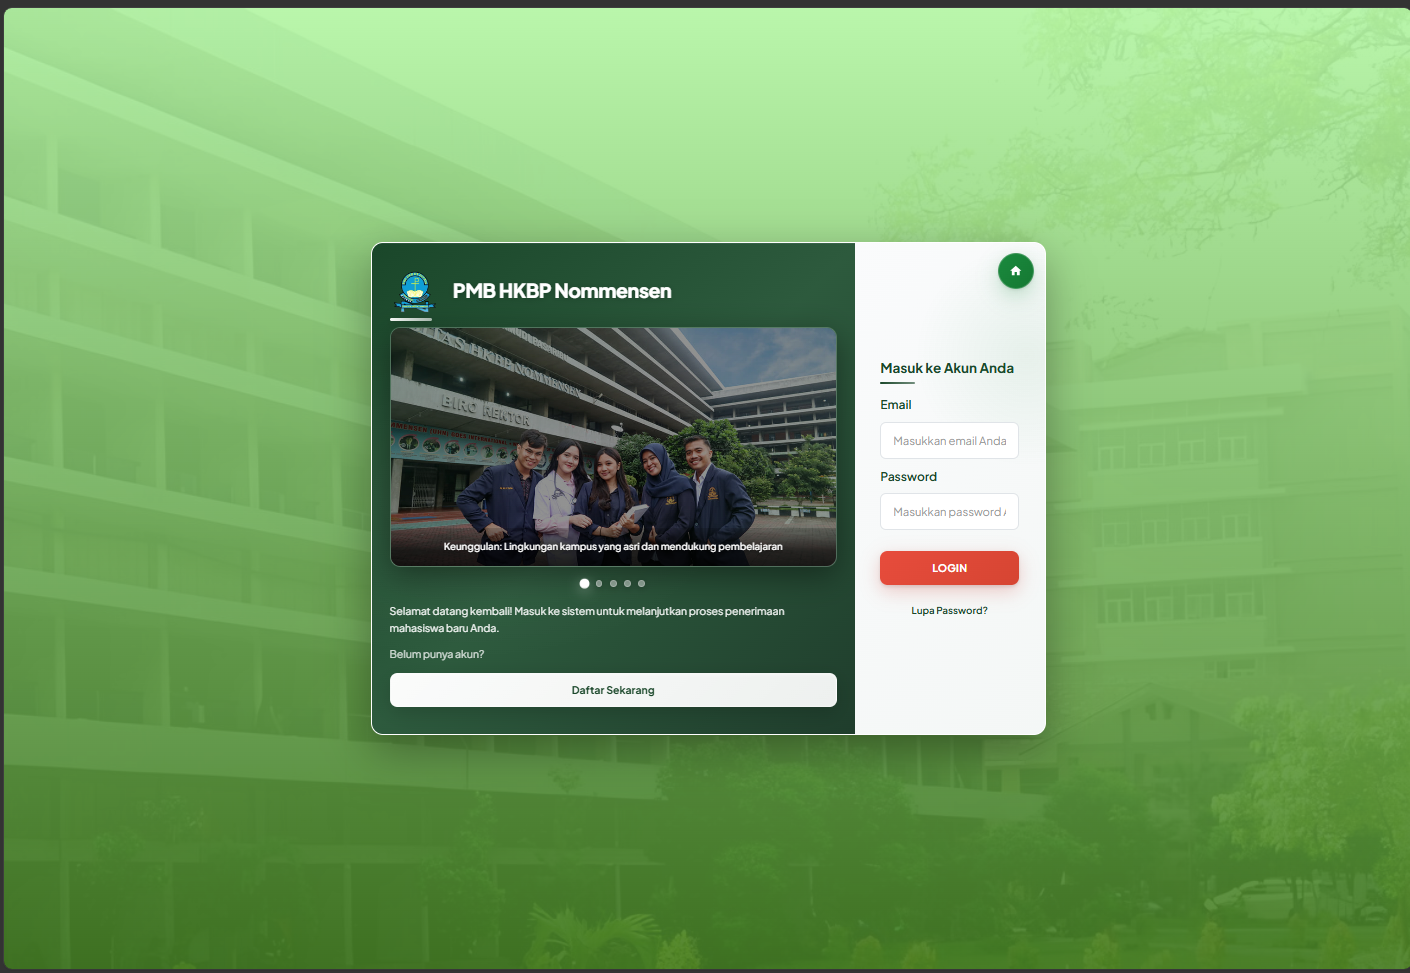
\includegraphics[width=0.7\textwidth]{figure/bab4/m-login.png}
	\caption{Halaman Login Sistem PMB}
	\label{fig:4.login}
\end{figure}

\begin{lstlisting}[language=Java, caption={Endpoint login yang menghasilkan token JWT berisi peran pengguna}, label={kode:4.login}]
// AuthController.java  -- POST /api/auth/login  (permitAll)
@PostMapping("/login")
public ResponseEntity<?> login(@Valid @RequestBody LoginRequest req) {
    // AuthService: 1) verifikasi email+password, 2) generate JWT(email+role)
    AuthResponse response = authService.login(req);
    return ResponseEntity.ok(response);
}
\end{lstlisting}

% ------------------------------------------------
\subsubsection{Modul 2 --- Halaman Registrasi} \label{IV.Mod.Register}
% ------------------------------------------------

Modul registrasi memungkinkan camaba membuat akun baru dengan mengisi nama lengkap, email, dan kata sandi. Pada prototipe awal, akun langsung diaktifkan setelah registrasi tanpa proses verifikasi email. Tampilan halaman registrasi ditunjukkan pada Gambar \ref{fig:4.register}.\par

\begin{figure}[H]
	\centering
	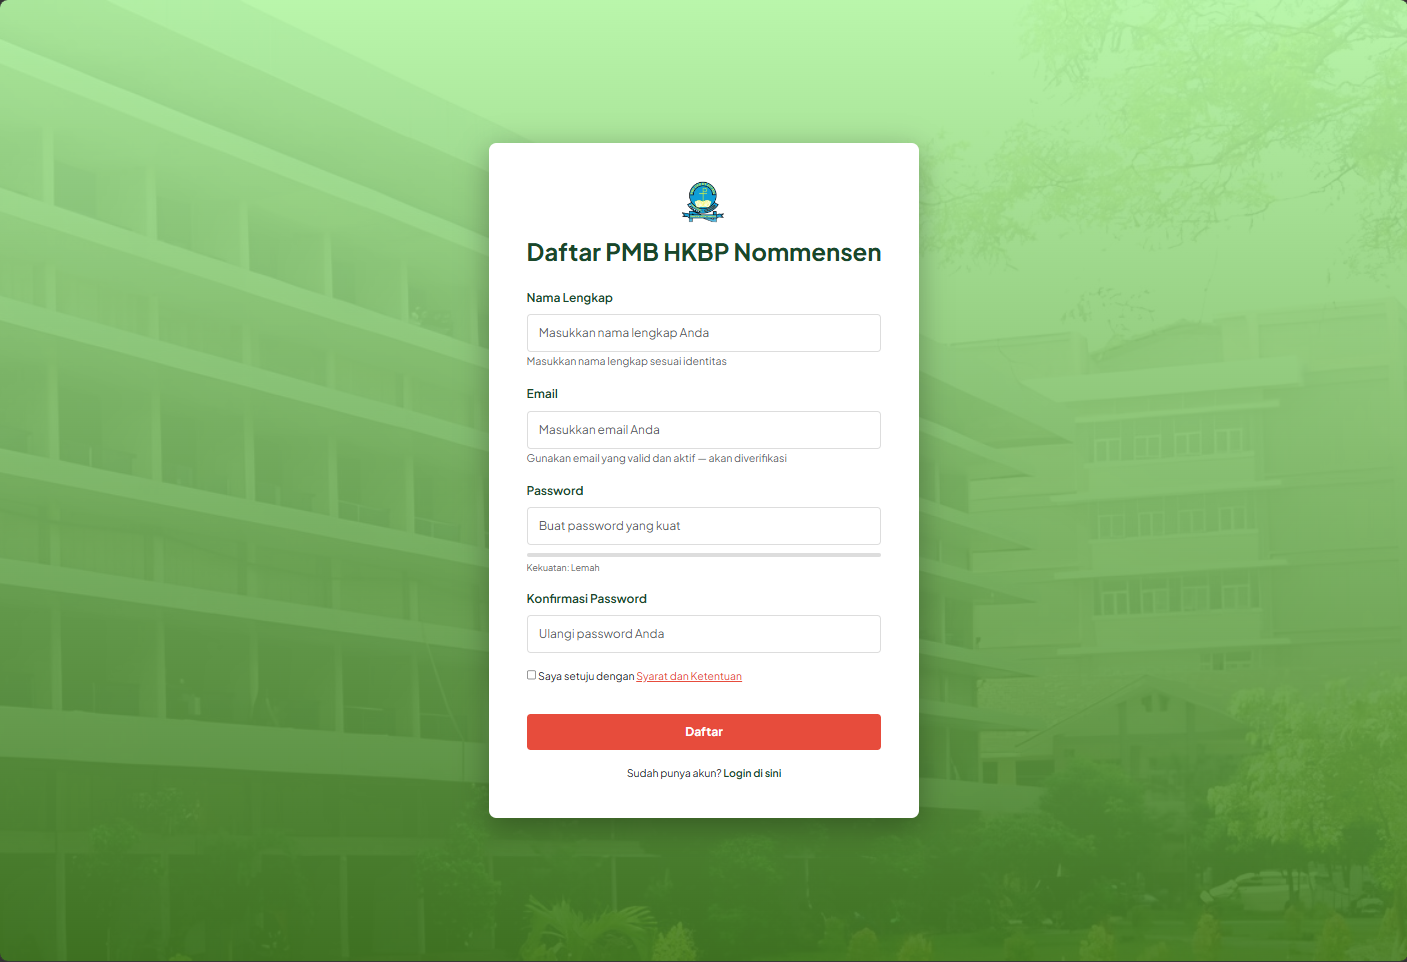
\includegraphics[width=0.75\textwidth]{figure/bab4/m-register.png}
	\caption{Halaman Registrasi Akun Camaba}
	\label{fig:4.register}
\end{figure}

\begin{lstlisting}[language=Java, caption={Endpoint registrasi akun camaba baru}, label={kode:4.register}]
// AuthController.java  -- POST /api/auth/register  (permitAll)
@PostMapping("/register")
public ResponseEntity<?> register(@Valid @RequestBody RegisterRequest req) {
    if (!req.getPassword().equals(req.getConfirmPassword()))
        return ResponseEntity.badRequest()
            .body(new ApiResponse(false, "Password tidak cocok"));
    // AuthService: 1) cek duplikat email, 2) hash password BCrypt,
    //              3) buat Student, 4) aktifkan akun langsung
    AuthResponse response = authService.register(req);
    return ResponseEntity.status(HttpStatus.CREATED).body(response);
}
\end{lstlisting}

% ------------------------------------------------
\subsubsection{Modul 3 --- Lupa dan Reset Kata Sandi} \label{IV.Mod.ForgotPw}
% ------------------------------------------------

Modul ini memungkinkan pengguna yang lupa kata sandi meminta tautan \textit{reset} melalui email. Tautan mengandung token unik satu kali pakai (\textit{one-time token}) dengan masa berlaku 1 jam. Tampilan halaman lupa kata sandi ditunjukkan pada Gambar \ref{fig:4.forgotpw}.\par

\begin{figure}[H]
	\centering
	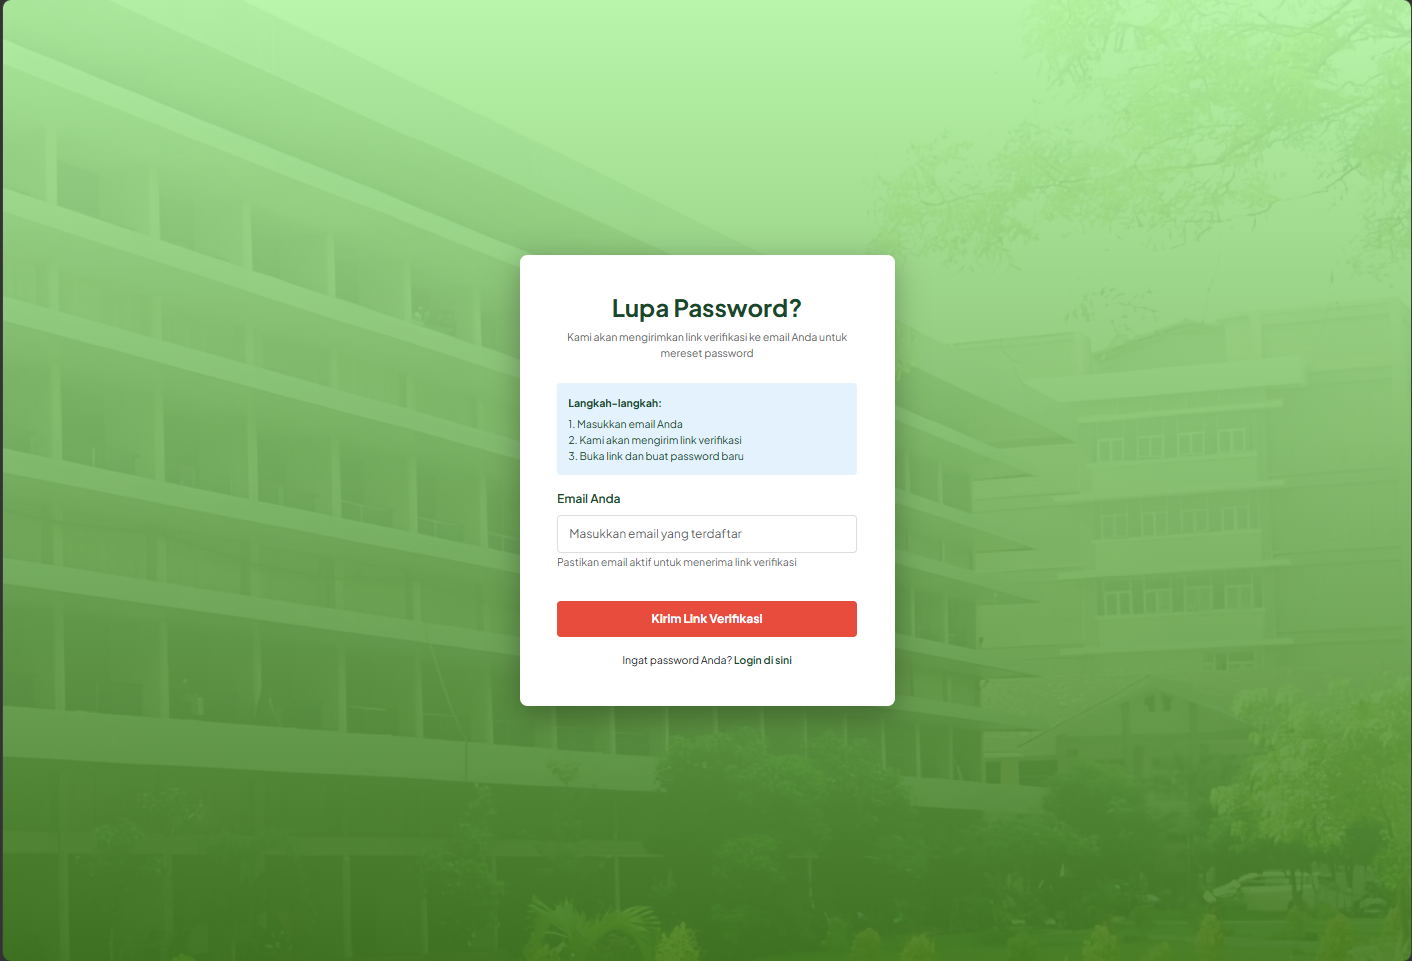
\includegraphics[width=0.7\textwidth]{figure/bab4/m-forgot-password.png}
	\caption{Halaman Lupa Kata Sandi dengan Verifikasi melalui Email}
	\label{fig:4.forgotpw}
\end{figure}

\begin{lstlisting}[language=Java, caption={Endpoint lupa dan reset kata sandi di AuthController}, label={kode:4.forgotpw}]
// AuthController.java  -- /api/auth/**  (permitAll)
@PostMapping("/forgot-password")
public ResponseEntity<?> forgotPassword(@RequestBody ForgotPasswordRequest req) {
    // Buat UUID token, simpan ke password_reset_tokens (expired +1 jam)
    // Kirim email berisi link: /reset-password?token=UUID
    authService.sendResetPasswordEmail(req.getEmail());
    return ResponseEntity.ok("Email reset kata sandi telah dikirim");
}
@PostMapping("/reset-password")
public ResponseEntity<?> resetPassword(@RequestBody ResetPasswordRequest req) {
    // Validasi token (ada, belum digunakan, belum expired)
    // Update password dengan BCrypt, tandai token used
    authService.resetPassword(req.getToken(), req.getNewPassword());
    return ResponseEntity.ok("Kata sandi berhasil diubah");
}
\end{lstlisting}

% ------------------------------------------------
\subsubsection{Modul 4 --- Pemilihan Gelombang dan Jenis Seleksi} \label{IV.Mod.Gelombang}
% ------------------------------------------------

Setelah login, langkah pertama camaba adalah memilih gelombang pendaftaran aktif dan jenis seleksi yang sesuai. Data gelombang berasal dari tabel \texttt{registration\_periods} yang dikelola Admin Pusat. Tampilan halaman pemilihan gelombang ditunjukkan pada Gambar \ref{fig:4.gelombang}.\par

\begin{figure}[H]
	\centering
	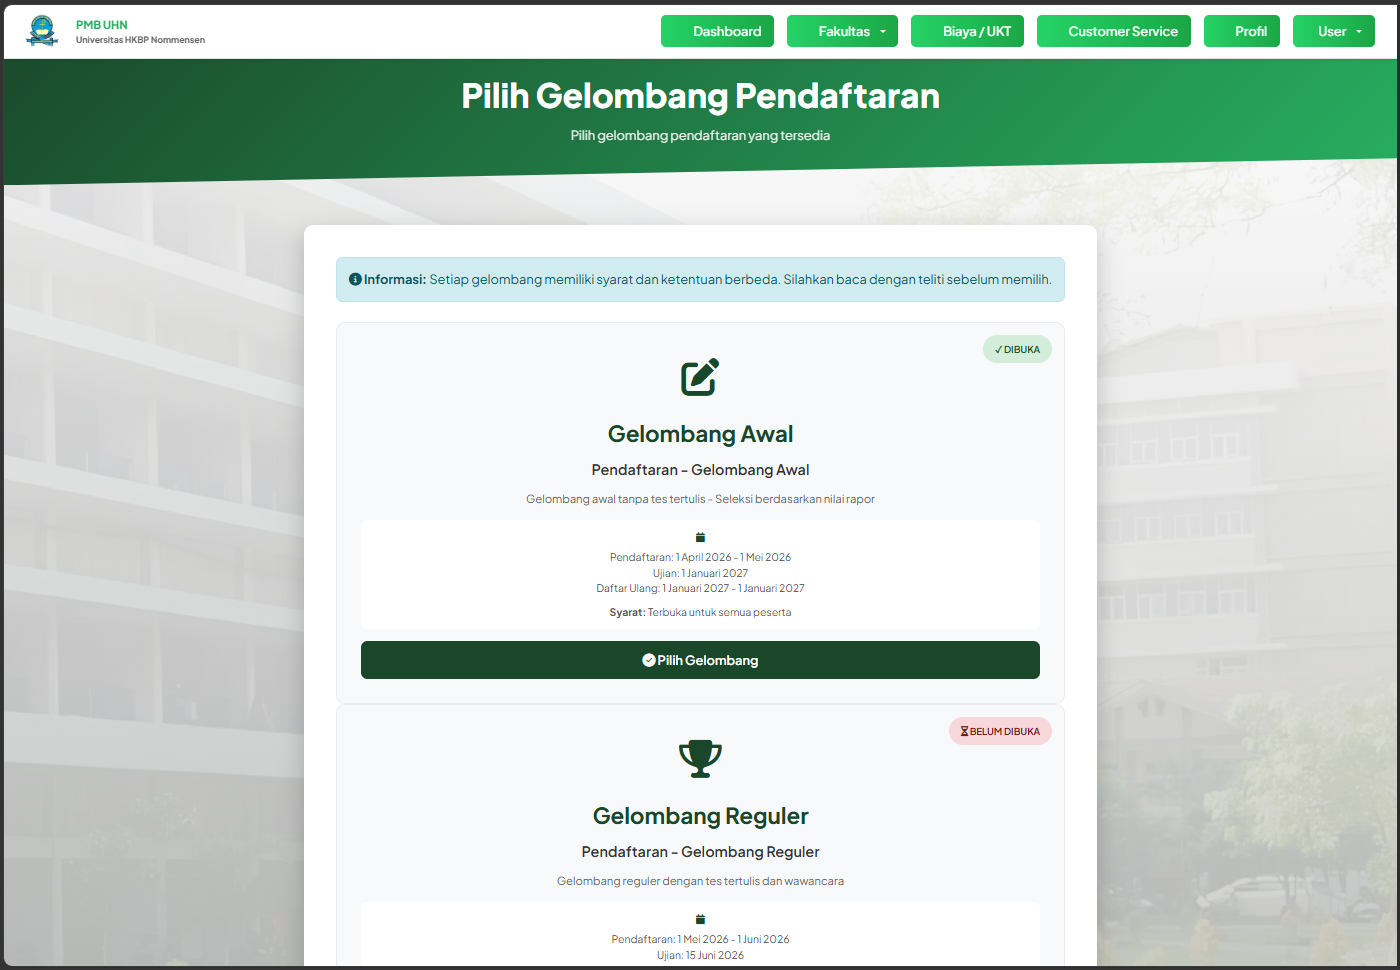
\includegraphics[width=0.85\textwidth]{figure/bab4/m-gelombang.png}
	\caption{Halaman Pemilihan Gelombang dan Jenis Seleksi}
	\label{fig:4.gelombang}
\end{figure}

\begin{lstlisting}[language=Java, caption={Endpoint pemilihan gelombang dan pengambilan jenis seleksi aktif}, label={kode:4.gelombang}]
// CamabaController.java  -- prefix: /api/camaba  (authenticated)
@GetMapping("/registration-periods")  // Ambil daftar gelombang aktif
public ResponseEntity<?> getRegistrationPeriods(Principal principal) {
    return ResponseEntity.ok(
        periodRepository.findByIsActiveTrue());
}
@PostMapping("/select-gelombang")
public ResponseEntity<?> selectGelombang(
        @RequestBody SelectGelombangRequest req, Principal principal) {
    // Simpan pilihan gelombang + jenis seleksi ke AdmissionForm camaba
    return ResponseEntity.ok(camabaService.selectGelombang(req, principal));
}
\end{lstlisting}

% ------------------------------------------------
\subsubsection{Modul 5 --- Pemilihan Metode Pembayaran} \label{IV.Mod.MetodePembayaran}
% ------------------------------------------------

Setelah memilih gelombang, camaba memilih metode pembayaran uang pendaftaran: (1) Virtual Account BRIVA, atau (2) transfer manual dengan unggah bukti. Pilihan ini menentukan alur pembayaran selanjutnya. Tampilan halaman pemilihan metode ditunjukkan pada Gambar \ref{fig:4.metodepembayaran}.\par

\begin{figure}[H]
	\centering
	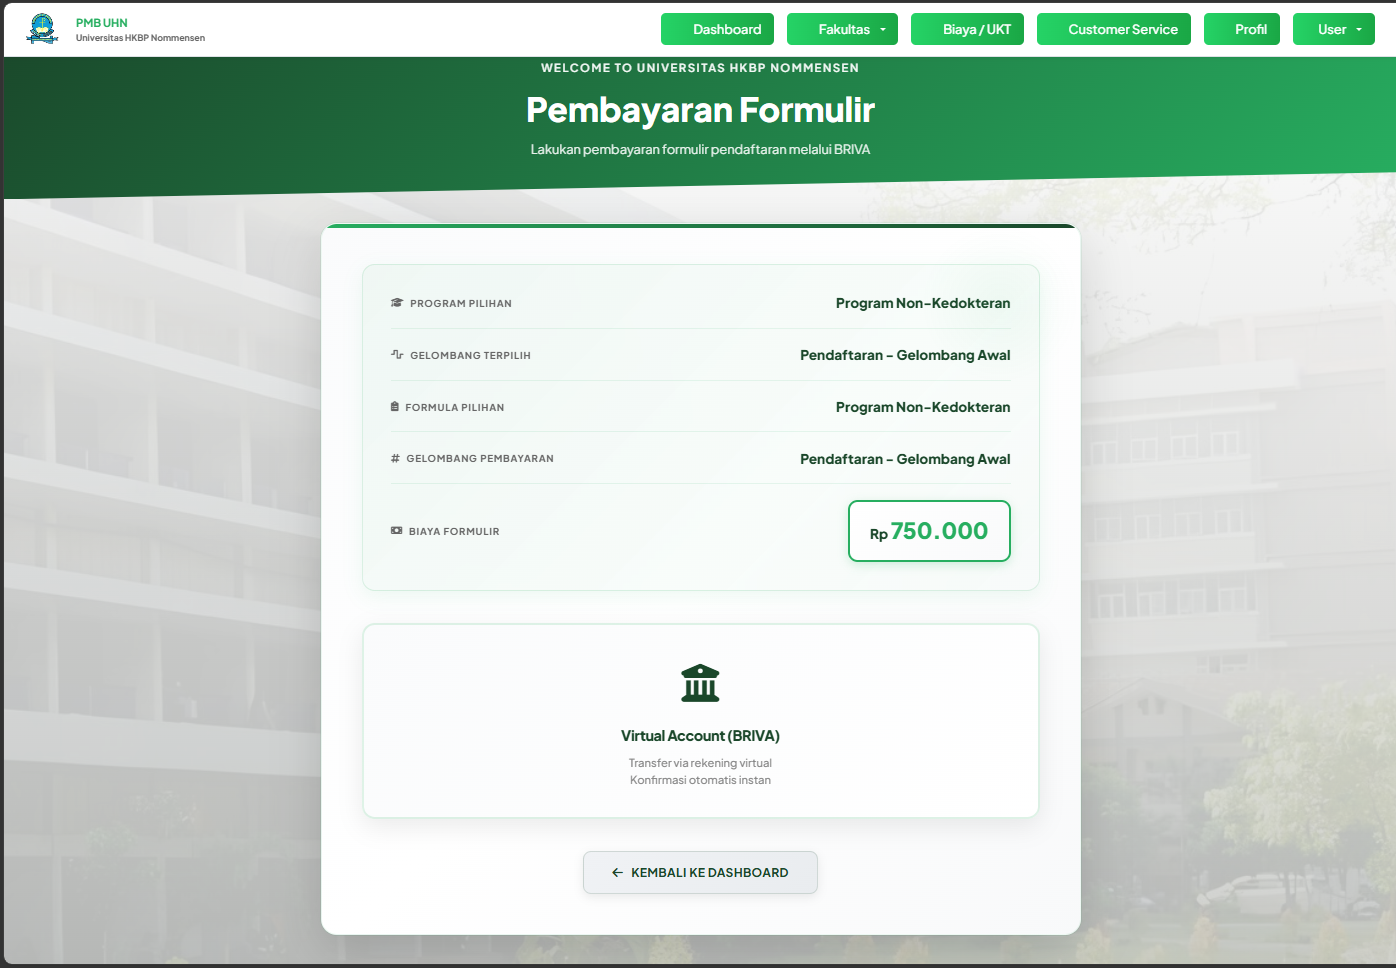
\includegraphics[width=0.8\textwidth]{figure/bab4/m-payment-method.png}
	\caption{Halaman Pemilihan Metode Pembayaran}
	\label{fig:4.metodepembayaran}
\end{figure}

\begin{lstlisting}[language=Java, caption={Endpoint pemilihan metode pembayaran di CamabaController}, label={kode:4.metodepembayaran}]
// CamabaController.java
@PostMapping("/select-formula")  // pilih jenis seleksi + metode bayar
public ResponseEntity<?> selectFormula(
        @RequestBody SelectFormulaRequest req, Principal principal) {
    // req.paymentMethod = "BRIVA" | "MANUAL" | "CICILAN"
    // Simpan ke AdmissionForm, kembalikan instruksi langkah berikutnya
    return ResponseEntity.ok(camabaService.selectFormula(req, principal));
}
\end{lstlisting}

% ------------------------------------------------
\subsubsection{Modul 6 --- Pembayaran BRIVA dan Upload Bukti Manual} \label{IV.Mod.Pembayaran}
% ------------------------------------------------

Modul ini menangani dua jalur pembayaran. Untuk BRIVA, sistem menampilkan nomor Virtual Account untuk ditransfer. Untuk manual, camaba mengunggah foto/PDF bukti transfer yang kemudian diverifikasi admin. Tampilan halaman pembayaran ditunjukkan pada Gambar \ref{fig:4.pembayaran}.\par

\begin{figure}[H]
	\centering
	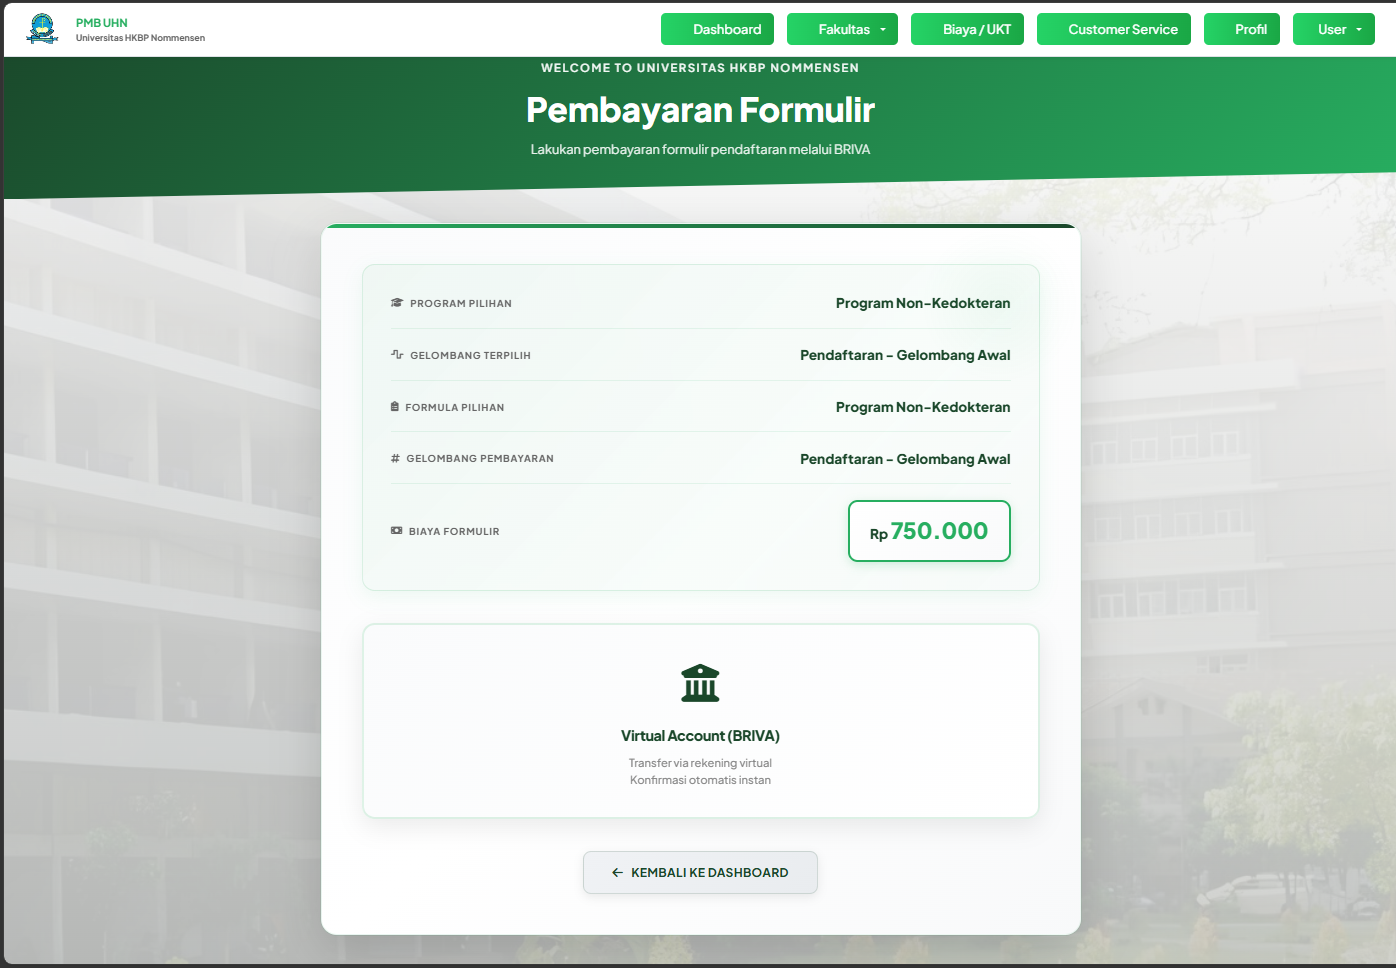
\includegraphics[width=0.85\textwidth]{figure/bab4/m-briva.png}
	\caption{Halaman Pembayaran BRIVA dan Unggah Bukti Transfer Manual}
	\label{fig:4.pembayaran}
\end{figure}

\begin{lstlisting}[language=Java, caption={Endpoint verifikasi pembayaran manual oleh admin di AdminController}, label={kode:4.pembayaran}]
// AdminController.java  -- PUT /admin/api/validasi/formulir/{id}/verify-payment
@PutMapping("/api/validasi/formulir/{id}/verify-payment")
@PreAuthorize("hasAnyRole('ADMIN_PUSAT', 'ADMIN_VALIDASI')")
public ResponseEntity<?> verifyPayment(@PathVariable Long id,
        @RequestBody VerifyPaymentRequest req) {
    // 1. Update status pembayaran: VERIFIED / REJECTED
    // 2. Jika VERIFIED: buka akses formulir pendaftaran
    // 3. Kirim email notifikasi ke camaba
    return ResponseEntity.ok(validasiService.verifyPayment(id, req));
}
\end{lstlisting}

% ------------------------------------------------
\subsubsection{Modul 7 --- Pengisian Formulir Pendaftaran} \label{IV.Mod.Formulir}
% ------------------------------------------------

Setelah pembayaran diverifikasi, camaba mengisi formulir pendaftaran multi-langkah yang mencakup data pribadi, informasi orang tua, asal sekolah, dan pilihan program studi hingga tiga pilihan. Pada prototipe awal, kolom asal sekolah berupa \textit{input} teks bebas tanpa \textit{autocomplete}. Tampilan formulir pendaftaran ditunjukkan pada Gambar \ref{fig:4.formulir}.\par

\begin{figure}[H]
	\centering
	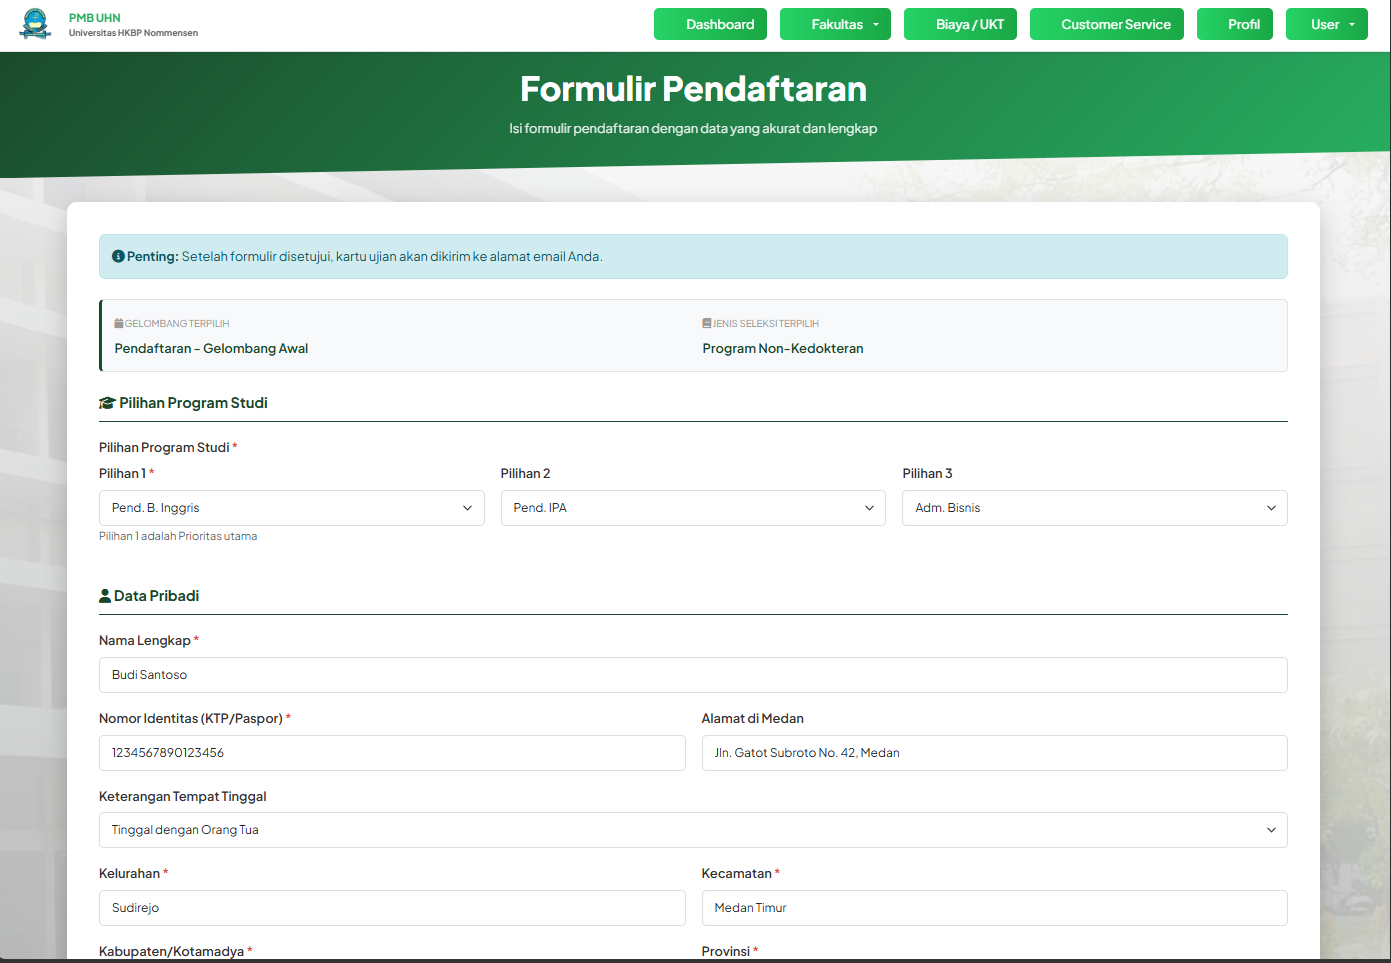
\includegraphics[width=0.9\textwidth]{figure/bab4/m-formulir.png}
	\caption{Halaman Pengisian Formulir Pendaftaran}
	\label{fig:4.formulir}
\end{figure}

\begin{lstlisting}[language=Java, caption={Endpoint pengiriman formulir pendaftaran camaba}, label={kode:4.formulir}]
// CamabaController.java
@PostMapping(value = "/admission-form", consumes = "multipart/form-data")
public ResponseEntity<?> submitAdmissionForm(
        @RequestPart("data") String jsonData,
        @RequestPart(value = "foto", required = false) MultipartFile foto,
        Principal principal) {
    // Validasi: pembayaran harus sudah terverifikasi
    // Simpan ke admission_forms dengan status SUBMITTED
    return ResponseEntity.ok(
        camabaService.submitAdmissionForm(jsonData, foto, principal));
}
\end{lstlisting}

% ------------------------------------------------
\subsubsection{Modul 8 --- Revisi Formulir} \label{IV.Mod.Revisi}
% ------------------------------------------------

Apabila admin menolak formulir karena dokumen tidak lengkap atau data tidak valid, camaba menerima notifikasi email berisi alasan penolakan dan dapat mengakses halaman revisi untuk melakukan perbaikan. Tampilan halaman revisi ditunjukkan pada Gambar \ref{fig:4.revisi}.\par

\begin{figure}[H]
	\centering
	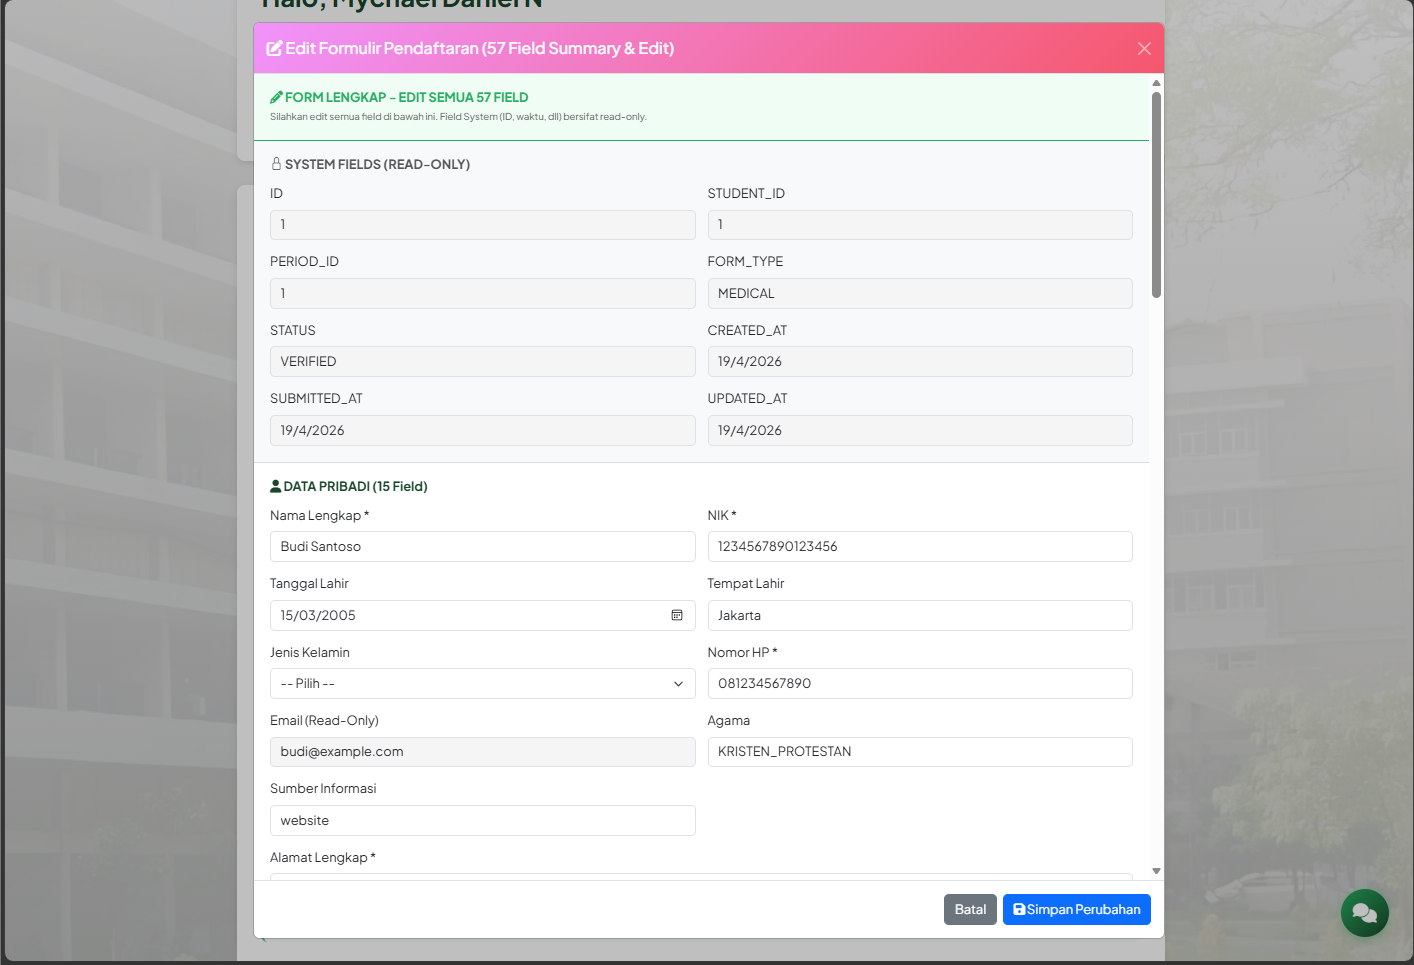
\includegraphics[width=0.85\textwidth]{figure/bab4/m-revisi.png}
	\caption{Halaman Revisi Formulir Setelah Penolakan}
	\label{fig:4.revisi}
\end{figure}

\begin{lstlisting}[language=Java, caption={Endpoint penolakan formulir dan pengiriman ulang revisi}, label={kode:4.revisi}]
// AdminController.java -- tolak formulir dengan alasan
@PutMapping("/api/validasi/formulir/{validationId}/reject")
@PreAuthorize("hasAnyRole('ADMIN_VALIDASI', 'ADMIN_PUSAT')")
public ResponseEntity<?> rejectFormulir(@PathVariable Long validationId,
        @RequestBody RejectRequest req) {
    // Set status = REJECTED, simpan alasan, kirim email ke camaba
    return ResponseEntity.ok(validasiService.rejectForm(validationId, req));
}
// CamabaController.java -- camaba kirim ulang setelah revisi
@PutMapping(value = "/admission-form", consumes = "multipart/form-data")
public ResponseEntity<?> updateAdmissionForm(
        @RequestPart("data") String jsonData,
        Principal principal) {
    // Validasi: status harus REVISION_NEEDED/REJECTED
    return ResponseEntity.ok(
        camabaService.updateAdmissionForm(jsonData, principal));
}
\end{lstlisting}

% ------------------------------------------------
\subsubsection{Modul 9 --- Profil Mahasiswa dan Ubah Kata Sandi} \label{IV.Mod.Profil}
% ------------------------------------------------

Modul profil memungkinkan camaba melihat dan memperbarui data diri serta mengubah kata sandi. Halaman ini juga menampilkan ringkasan status pendaftaran. Tampilan halaman profil ditunjukkan pada Gambar \ref{fig:4.profil}.\par

\begin{figure}[H]
	\centering
	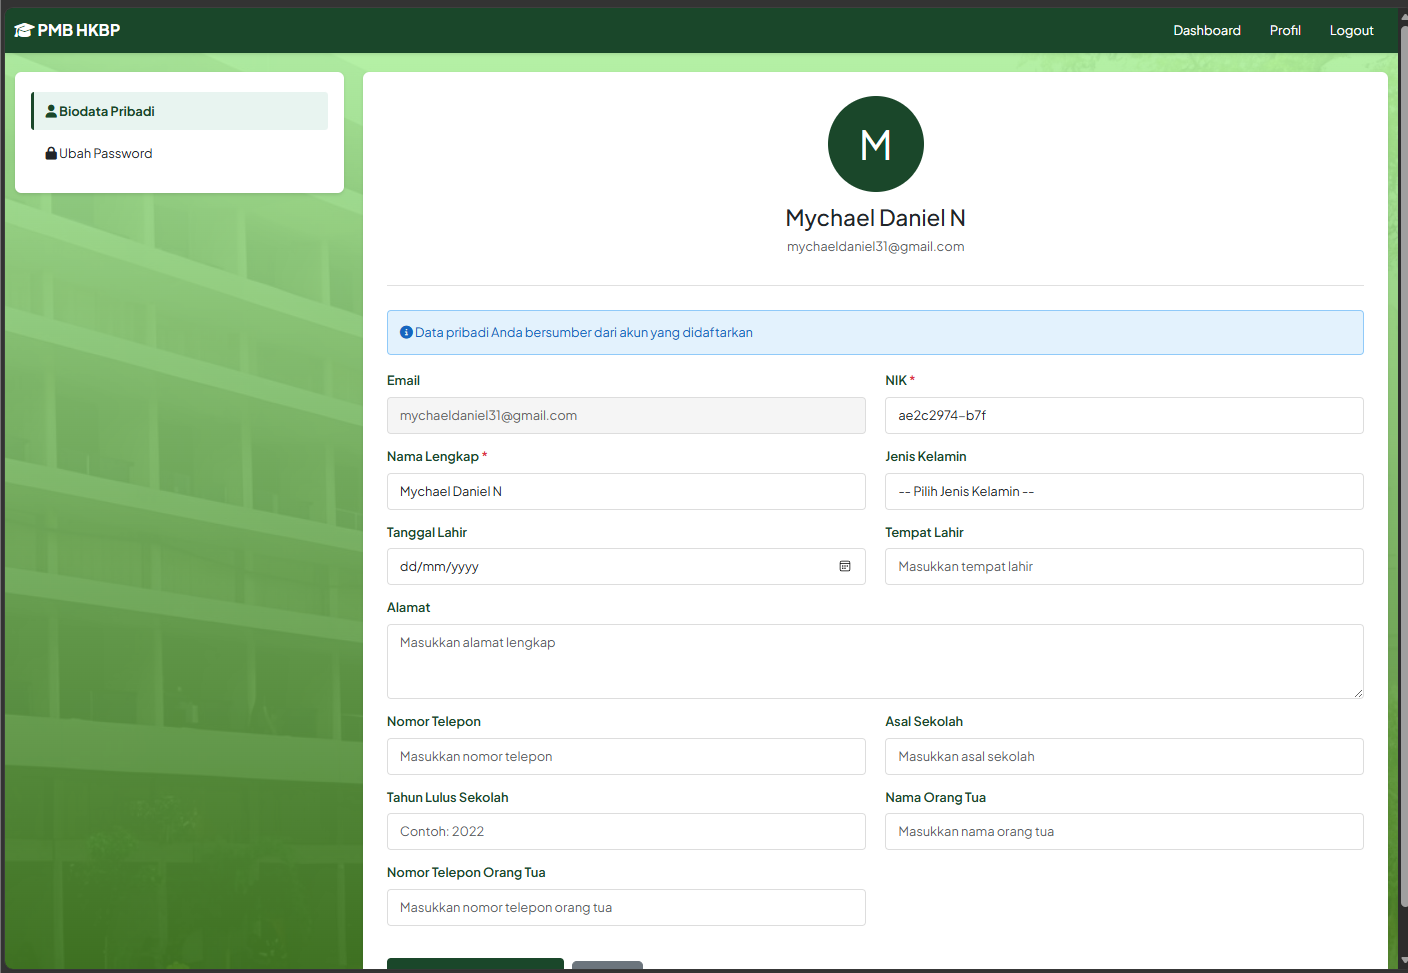
\includegraphics[width=0.85\textwidth]{figure/bab4/m-profil.png}
	\caption{Halaman Profil Mahasiswa}
	\label{fig:4.profil}
\end{figure}

\begin{lstlisting}[language=Java, caption={Endpoint profil camaba yang dilindungi JWT via Principal}, label={kode:4.profil}]
// CamabaController.java  -- /api/camaba/profile  (authenticated)
// Principal diisi otomatis oleh Spring Security dari SecurityContext
// yang di-set oleh JwtAuthenticationFilter pada setiap request
@GetMapping("/profile")
public ResponseEntity<?> getProfile(Principal principal) {
    return ResponseEntity.ok(camabaService.getProfile(principal.getName()));
}
@PutMapping("/profile")
public ResponseEntity<?> updateProfile(
        @RequestBody UpdateProfileRequest req, Principal principal) {
    return ResponseEntity.ok(
        camabaService.updateProfile(req, principal.getName()));
}
\end{lstlisting}

% ------------------------------------------------
\subsubsection{Modul 10 --- Pelacak Status Pendaftaran} \label{IV.Mod.StatusTracker}
% ------------------------------------------------

Modul ini menyediakan tampilan \textit{tracker} multi-tahap yang memungkinkan camaba melihat posisi mereka dalam alur pendaftaran secara visual. Setiap tahap (Pembayaran $\rightarrow$ Formulir $\rightarrow$ Ujian $\rightarrow$ Daftar Ulang $\rightarrow$ Hasil) ditampilkan dengan indikator status. Tampilan \textit{tracker} ditunjukkan pada Gambar \ref{fig:4.tracker}.\par

\begin{figure}[H]
	\centering
	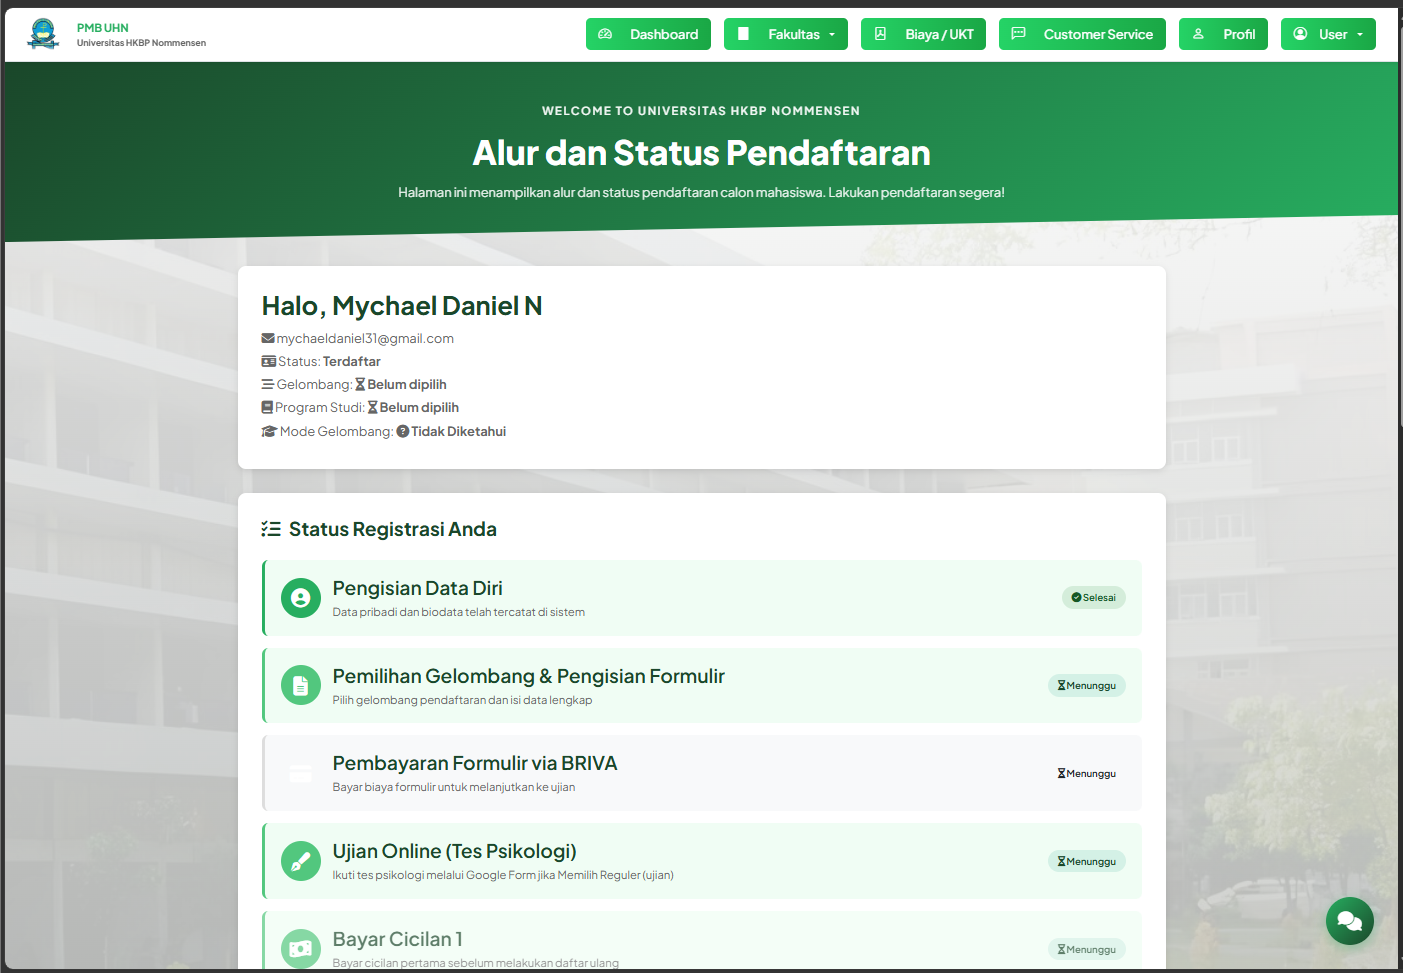
\includegraphics[width=0.85\textwidth]{figure/bab4/m-tracker.png}
	\caption{Pelacak Status Pendaftaran Multi-Tahap di Dasbor Camaba}
	\label{fig:4.tracker}
\end{figure}

\begin{lstlisting}[language=Java, caption={Endpoint status pendaftaran yang mengagregasi data dari berbagai tabel}, label={kode:4.tracker}]
// RegistrationStatusController.java
@GetMapping("/api/registration-status/my-status")
public ResponseEntity<?> getMyStatus(Principal principal) {
    // Mengagregasi status dari:
    // form_validations (bayar, formulir), exams (ujian), re_enrollments
    return ResponseEntity.ok(
        statusService.getStatusLengkap(principal.getName()));
}
\end{lstlisting}

% ------------------------------------------------
\subsubsection{Modul 11 --- Ujian Seleksi} \label{IV.Mod.Ujian}
% ------------------------------------------------

Setelah formulir disetujui, camaba mengikuti ujian seleksi. Sistem mendukung dua mode: ujian \textit{online} melalui tautan Google Form yang dikonfigurasi admin per gelombang, dan ujian \textit{offline} di mana camaba mengunggah bukti kehadiran. Pada prototipe awal, admin dapat melihat pengumpulan ujian namun belum ada mekanisme penetapan lulus/tidak lulus secara eksplisit. Tampilan halaman ujian ditunjukkan pada Gambar \ref{fig:4.ujian}.\par

\begin{figure}[H]
	\centering
	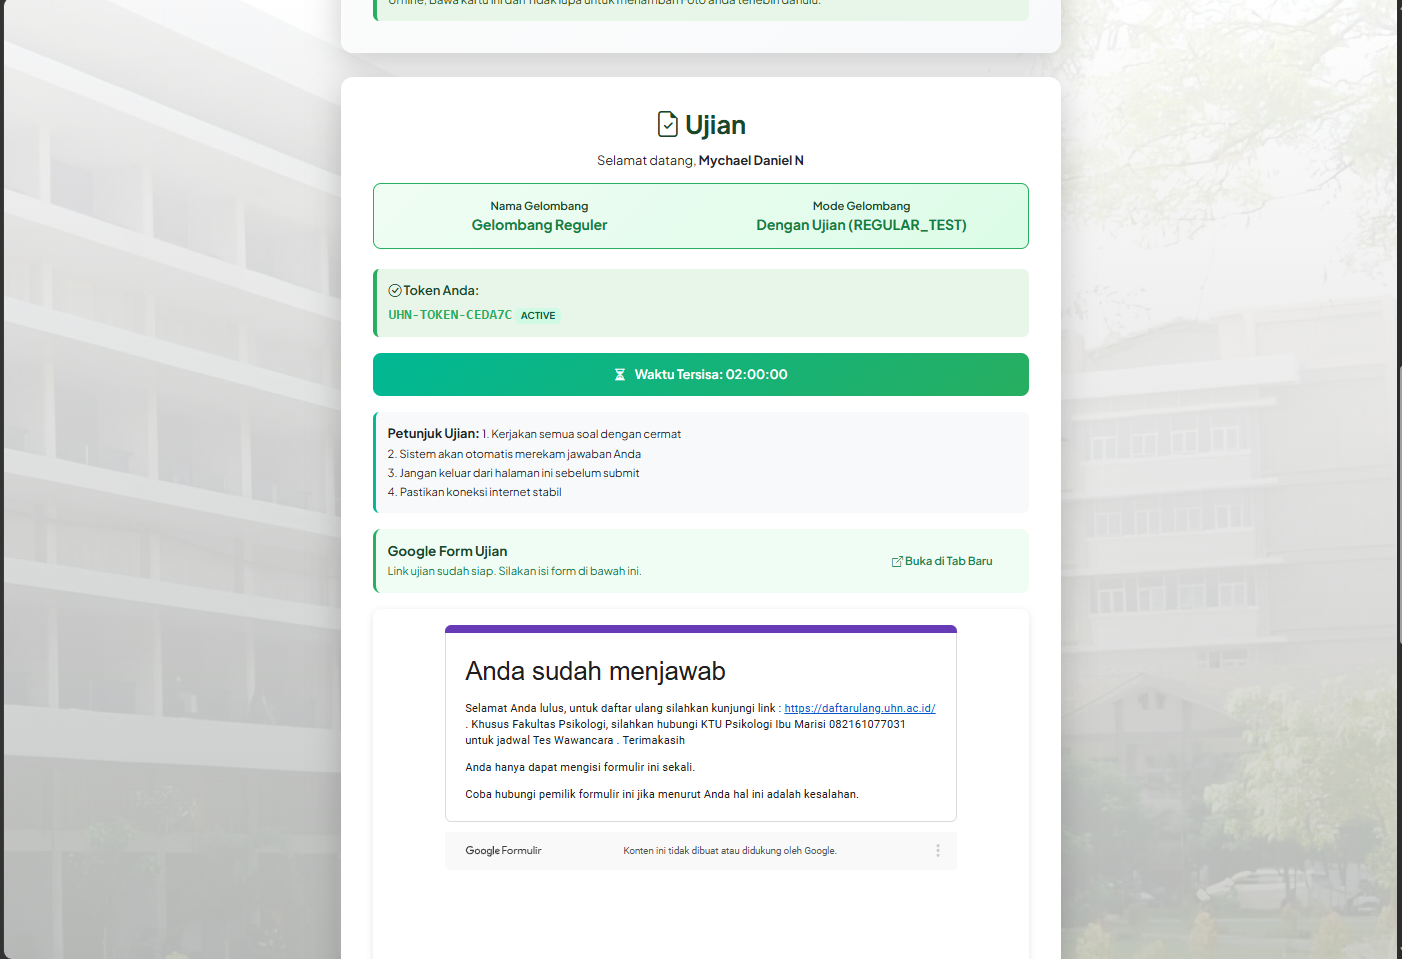
\includegraphics[width=0.85\textwidth]{figure/bab4/m-ujian.png}
	\caption{Halaman Ujian Seleksi Mode Online dan Offline}
	\label{fig:4.ujian}
\end{figure}

\begin{lstlisting}[language=Java, caption={Endpoint pengumpulan ujian oleh camaba di CamabaController}, label={kode:4.ujian}]
// CamabaController.java  -- POST /api/camaba/submit-exam
@PostMapping("/submit-exam")
public ResponseEntity<?> submitExam(
        @RequestBody SubmitExamRequest req, Principal principal) {
    // Simpan ExamSubmission: waktu, token, file bukti (offline)
    // Update status camaba: ujian selesai
    return ResponseEntity.ok(camabaService.submitExam(req, principal));
}
\end{lstlisting}

% ------------------------------------------------
\subsubsection{Modul 12 --- Pengajuan Cicilan} \label{IV.Mod.Cicilan}
% ------------------------------------------------

Camaba yang tidak mampu membayar lunas dapat mengajukan cicilan melalui halaman khusus. Pada prototipe awal, cicilan bersifat permintaan sederhana tanpa konfigurasi jumlah tahap---admin yang menentukan skema cicilan secara manual setelah menyetujui pengajuan. Tampilan halaman cicilan ditunjukkan pada Gambar \ref{fig:4.cicilan}.\par

\begin{figure}[H]
	\centering
	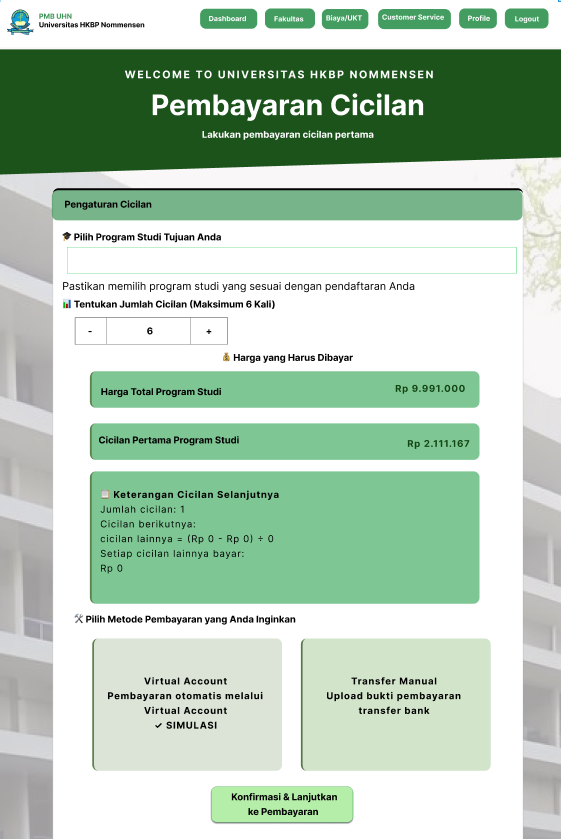
\includegraphics[width=0.85\textwidth]{figure/bab4/m-cicilan.png}
	\caption{Halaman Pengajuan Cicilan Camaba}
	\label{fig:4.cicilan}
\end{figure}

\begin{lstlisting}[language=Java, caption={Endpoint pengajuan cicilan dan pengecekan status di CicilanRequestController}, label={kode:4.cicilan}]
// CicilanRequestController.java  -- /api/cicilan
@PostMapping("/submit")
public ResponseEntity<?> submitCicilan(
        @RequestBody CicilanRequest req, Principal principal) {
    // Simpan cicilan_request dengan status PENDING
    // Admin Pusat / Admin Validasi dapat approve/reject via AdminCicilanController
    return ResponseEntity.ok(cicilanService.submit(req, principal));
}
@GetMapping("/my-status")
public ResponseEntity<?> myCicilanStatus(Principal principal) {
    return ResponseEntity.ok(cicilanService.getMyStatus(principal.getName()));
}
\end{lstlisting}

% ------------------------------------------------
\subsubsection{Modul 13 --- Daftar Ulang} \label{IV.Mod.DaftarUlang}
% ------------------------------------------------

Camaba yang dinyatakan lulus ujian seleksi wajib melakukan daftar ulang dengan mengunggah dokumen persyaratan (foto, KTP, ijazah, dll.). Admin Validasi memverifikasi kelengkapan dokumen tersebut. Tampilan halaman daftar ulang ditunjukkan pada Gambar \ref{fig:4.daftarulang}.\par

\begin{figure}[H]
	\centering
	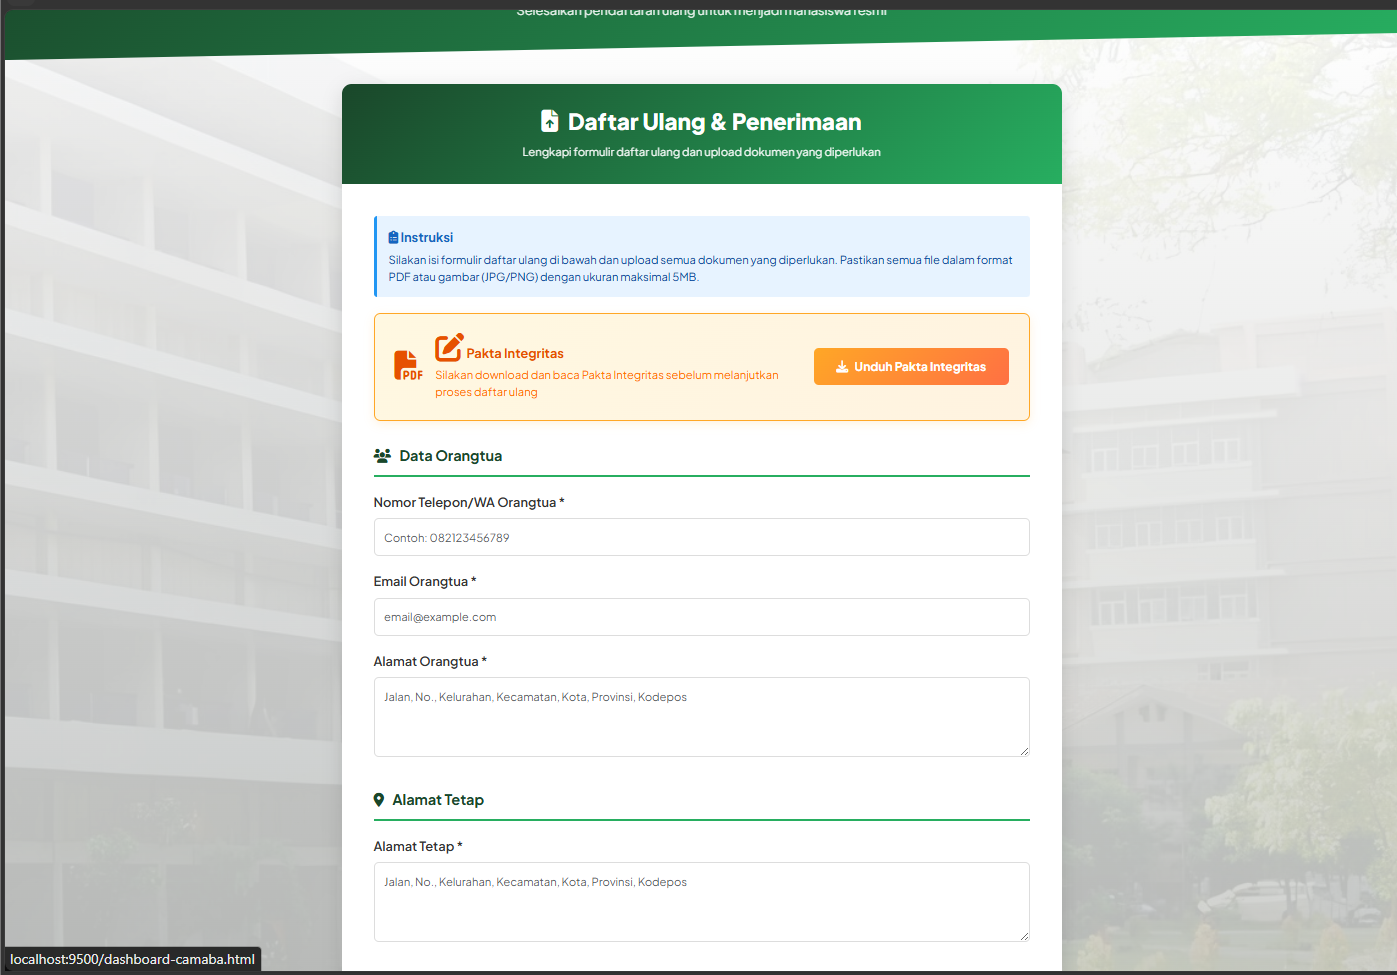
\includegraphics[width=0.9\textwidth]{figure/bab4/m-daftar-ulang.png}
	\caption{Halaman Daftar Ulang dan Unggah Dokumen Persyaratan}
	\label{fig:4.daftarulang}
\end{figure}

\begin{lstlisting}[language=Java, caption={Endpoint upload dokumen daftar ulang di CamabaController}, label={kode:4.daftarulang}]
// CamabaController.java (atau StudentController)
@PostMapping(value = "/reenrollment/upload",
             consumes = "multipart/form-data")
public ResponseEntity<?> uploadDokumenDaftarUlang(
        @RequestParam("file") MultipartFile file,
        @RequestParam("tipeDoc") String tipeDoc,
        Principal principal) {
    // Validasi tipe file: PDF, JPG, PNG (max 5 MB)
    // Simpan ke: uploads/daftar-ulang/{studentId}/{tipeDoc}/
    // Catat path di tabel re_enrollment_documents
    return ResponseEntity.ok(
        reenrollService.uploadDoc(file, tipeDoc, principal));
}
\end{lstlisting}

% ------------------------------------------------
\subsubsection{Modul 14 --- Hasil Akhir} \label{IV.Mod.HasilAkhir}
% ------------------------------------------------

Setelah daftar ulang terverifikasi, admin menetapkan hasil akhir camaba: nomor BRIVA final dan nomor registrasi. Camaba dapat melihat rekaman hasil akhir melalui dasbor. Pada prototipe awal, belum tersedia fitur unggah dan unduh NPM/KTM Sementara (ditambahkan pada Iterasi 1). Tampilan modal Hasil Akhir ditunjukkan pada Gambar \ref{fig:4.hasilakhir}.\par

\begin{figure}[H]
	\centering
	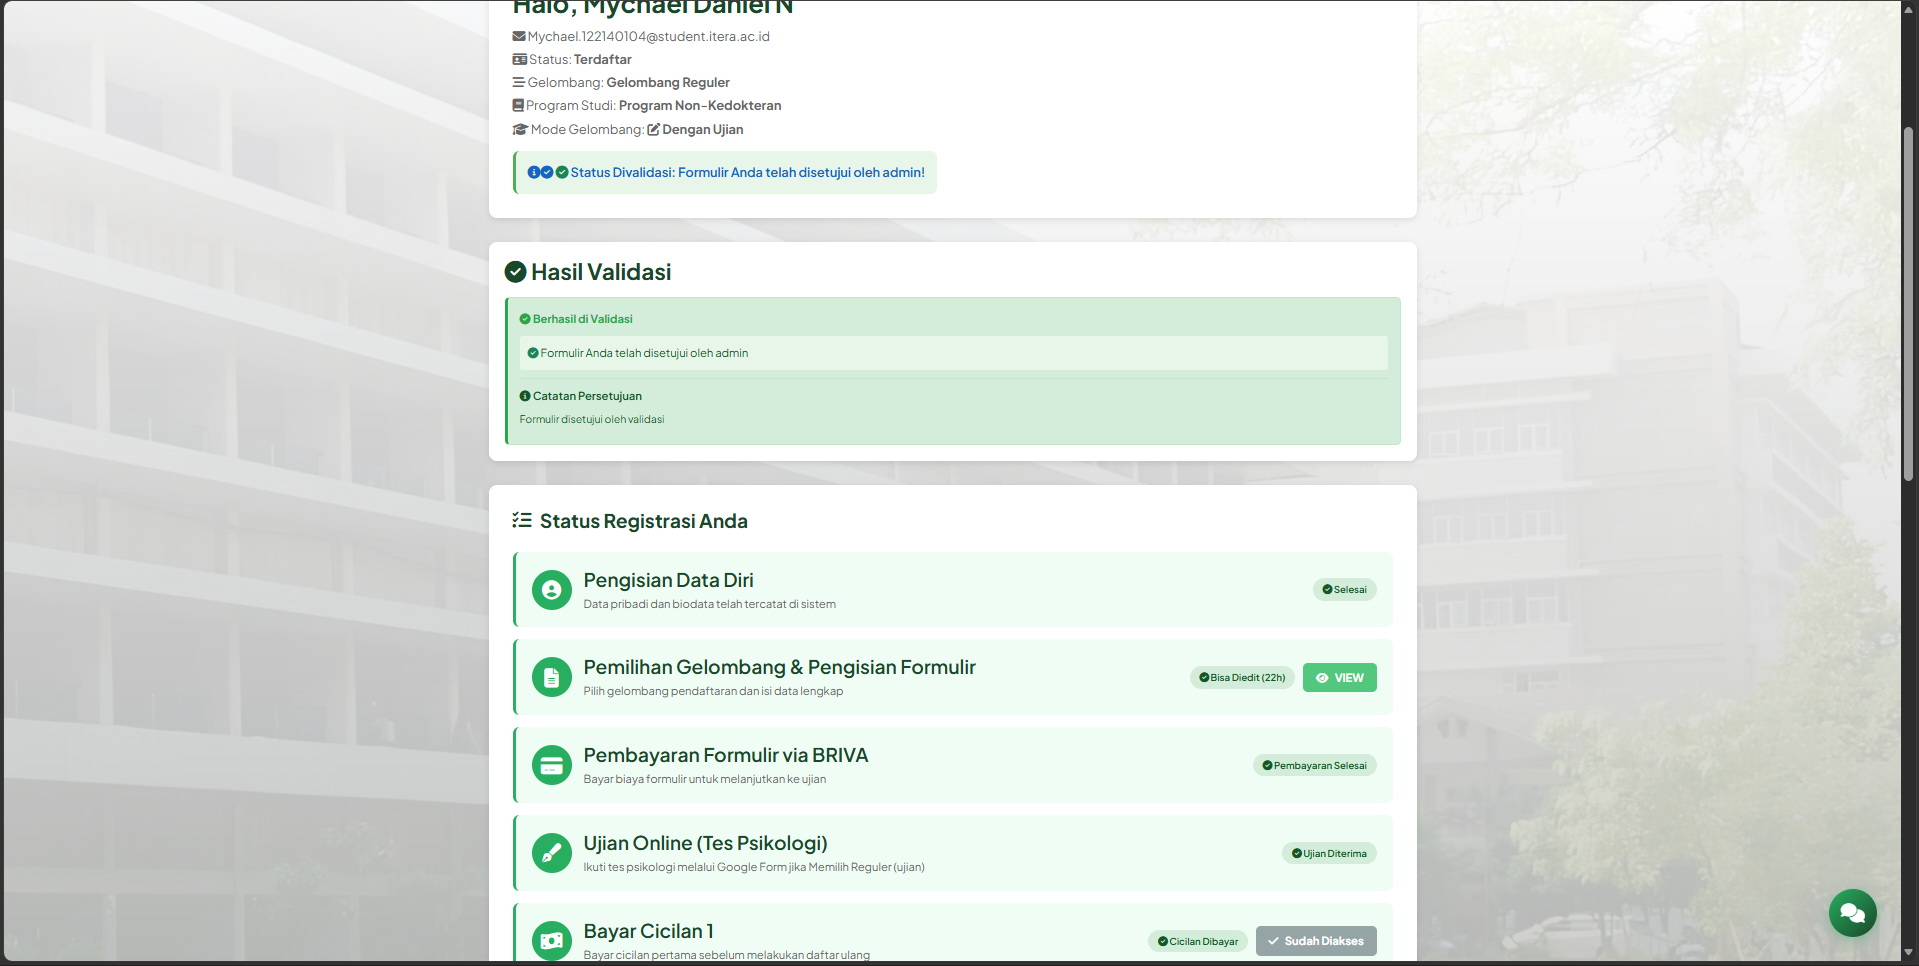
\includegraphics[width=0.85\textwidth]{figure/bab4/m-hasil-akhir.png}
	\caption{Modal Hasil Akhir di Dasbor Camaba}
	\label{fig:4.hasilakhir}
\end{figure}

\begin{lstlisting}[language=Java, caption={Endpoint penetapan nomor registrasi pada HasilAkhir oleh admin}, label={kode:4.hasilakhir}]
// AdminController.java
@PutMapping("/api/hasil-akhir/nomor-registrasi/{formValidationId}")
@PreAuthorize("hasAnyRole('ADMIN_VALIDASI', 'ADMIN_PUSAT')")
public ResponseEntity<?> setNomorRegistrasi(
        @PathVariable Long formValidationId,
        @RequestBody NomorRegistrasiRequest req) {
    // Ambil atau buat HasilAkhir untuk camaba ini
    // Set nomorRegistrasi jika tidak kosong;
    // auto-generate "REG-YYYYMMDD-NNNNNN" sebagai fallback
    return ResponseEntity.ok(
        hasilAkhirService.setNomorRegistrasi(formValidationId, req));
}
\end{lstlisting}

% ------------------------------------------------
\subsubsection{Modul 15 --- Manajemen Gelombang (Admin)} \label{IV.Mod.AdminGelombang}
% ------------------------------------------------

Admin Pusat dapat mengelola seluruh data gelombang pendaftaran: membuat gelombang baru, mengubah jadwal, mengaktifkan/menonaktifkan, dan menerbitkan hasil seleksi per gelombang. Tampilan manajemen gelombang di dasbor Admin ditunjukkan pada Gambar \ref{fig:4.admin_gelombang}.\par

\begin{figure}[H]
	\centering
	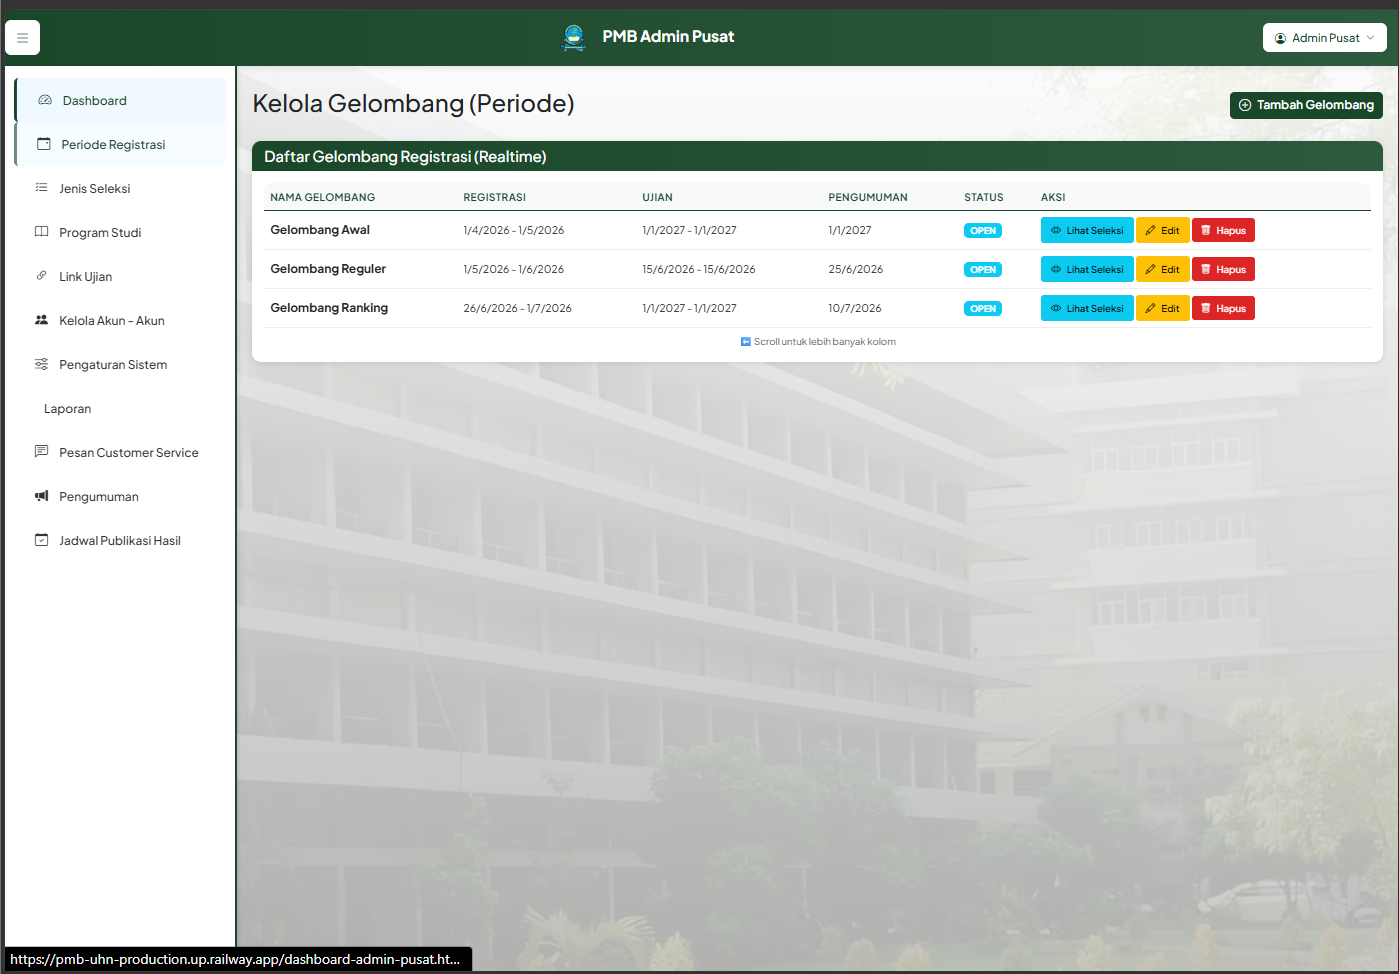
\includegraphics[width=0.9\textwidth]{figure/bab4/m-admin-gelombang.png}
	\caption{Halaman Manajemen Gelombang Pendaftaran di Dasbor Admin Pusat}
	\label{fig:4.admin_gelombang}
\end{figure}

\begin{lstlisting}[language=Java, caption={Endpoint CRUD gelombang pendaftaran dan publikasi hasil seleksi}, label={kode:4.admin_gelombang}]
// AdminController.java  -- prefix: /admin/api  (authenticated)
@PostMapping("/periods")   // Buat gelombang baru
@PreAuthorize("hasRole('ADMIN_PUSAT')")
public ResponseEntity<?> createPeriod(@RequestBody PeriodRequest req) {
    return ResponseEntity.ok(periodService.create(req));
}
@PutMapping("/periods/{id}")  // Edit gelombang
@PreAuthorize("hasRole('ADMIN_PUSAT')")
public ResponseEntity<?> updatePeriod(@PathVariable Long id,
        @RequestBody PeriodRequest req) {
    return ResponseEntity.ok(periodService.update(id, req));
}
@PostMapping("/publish-results/{periodId}")  // Publikasi hasil seleksi
@PreAuthorize("hasRole('ADMIN_PUSAT')")
public ResponseEntity<?> publishResults(@PathVariable Long periodId) {
    return ResponseEntity.ok(periodService.publishResults(periodId));
}
\end{lstlisting}

% ------------------------------------------------
\subsubsection{Modul 16 --- Manajemen Jenis Seleksi dan Program Studi (Admin)} \label{IV.Mod.AdminJenisSeleksi}
% ------------------------------------------------

Admin Pusat dapat mengelola jenis seleksi per gelombang (misalnya: Reguler, Kedokteran, Beasiswa) beserta program studi yang terkait. Manajemen program studi mencakup nama, harga, kuota, dan status aktif. Tampilan manajemen jenis seleksi ditunjukkan pada Gambar \ref{fig:4.admin_jenisseleksi}.\par

\begin{figure}[H]
	\centering
	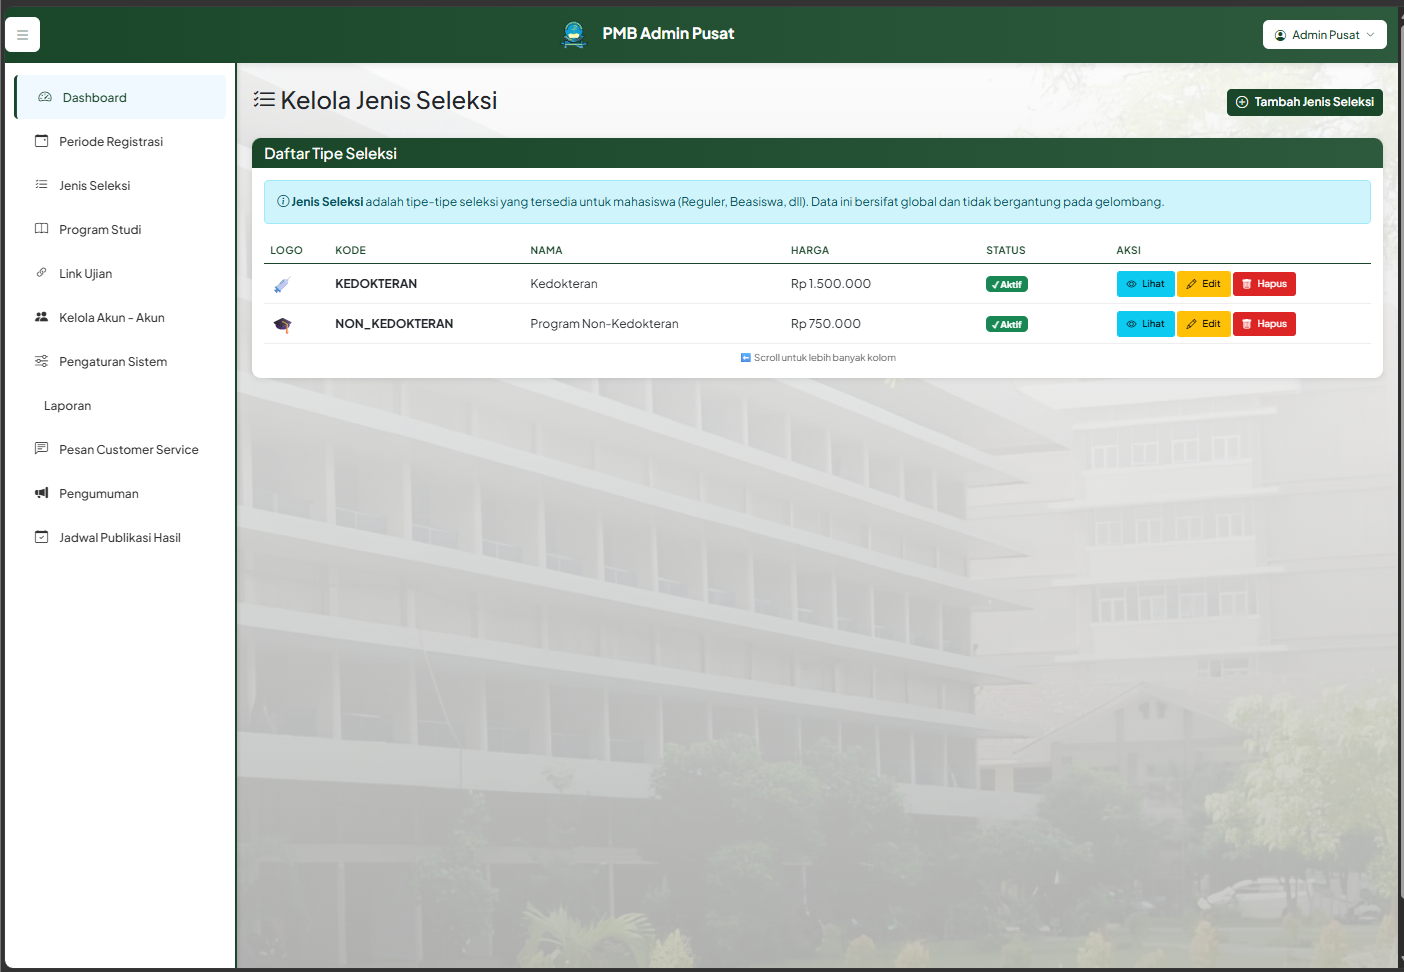
\includegraphics[width=0.9\textwidth]{figure/bab4/m-admin-jenis-seleksi.png}
	\caption{Halaman Manajemen Jenis Seleksi dan Program Studi}
	\label{fig:4.admin_jenisseleksi}
\end{figure}

\begin{lstlisting}[language=Java, caption={Endpoint CRUD jenis seleksi dan program studi di AdminController}, label={kode:4.admin_jenisseleksi}]
// AdminController.java  -- hanya ADMIN_PUSAT
@PostMapping("/jenis-seleksi")
@PreAuthorize("hasRole('ADMIN_PUSAT')")
public ResponseEntity<?> createJenisSeleksi(
        @RequestBody JenisSeleksiRequest req) {
    return ResponseEntity.ok(jenisSeleksiService.create(req));
}
@PostMapping("/program-studi")
@PreAuthorize("hasRole('ADMIN_PUSAT')")
public ResponseEntity<?> createProgramStudi(
        @RequestBody ProgramStudiRequest req) {
    return ResponseEntity.ok(programStudiService.create(req));
}
@GetMapping("/program-studi")
@PreAuthorize("hasAnyRole('ADMIN_PUSAT', 'ADMIN_VALIDASI')")
public ResponseEntity<?> getAllProgramStudi() {
    return ResponseEntity.ok(programStudiService.getAll());
}
\end{lstlisting}

% ------------------------------------------------
\subsubsection{Modul 17 --- Validasi Formulir Pendaftaran (Admin)} \label{IV.Mod.AdminValidasi}
% ------------------------------------------------

Admin Validasi dapat melihat daftar formulir yang masuk, memeriksa kelengkapan data dan dokumen, lalu menyetujui, menolak, atau meminta revisi. Setiap tindakan memicu notifikasi email otomatis ke camaba. Tampilan panel validasi formulir ditunjukkan pada Gambar \ref{fig:4.admin_validasi}.\par

\begin{figure}[H]
	\centering
	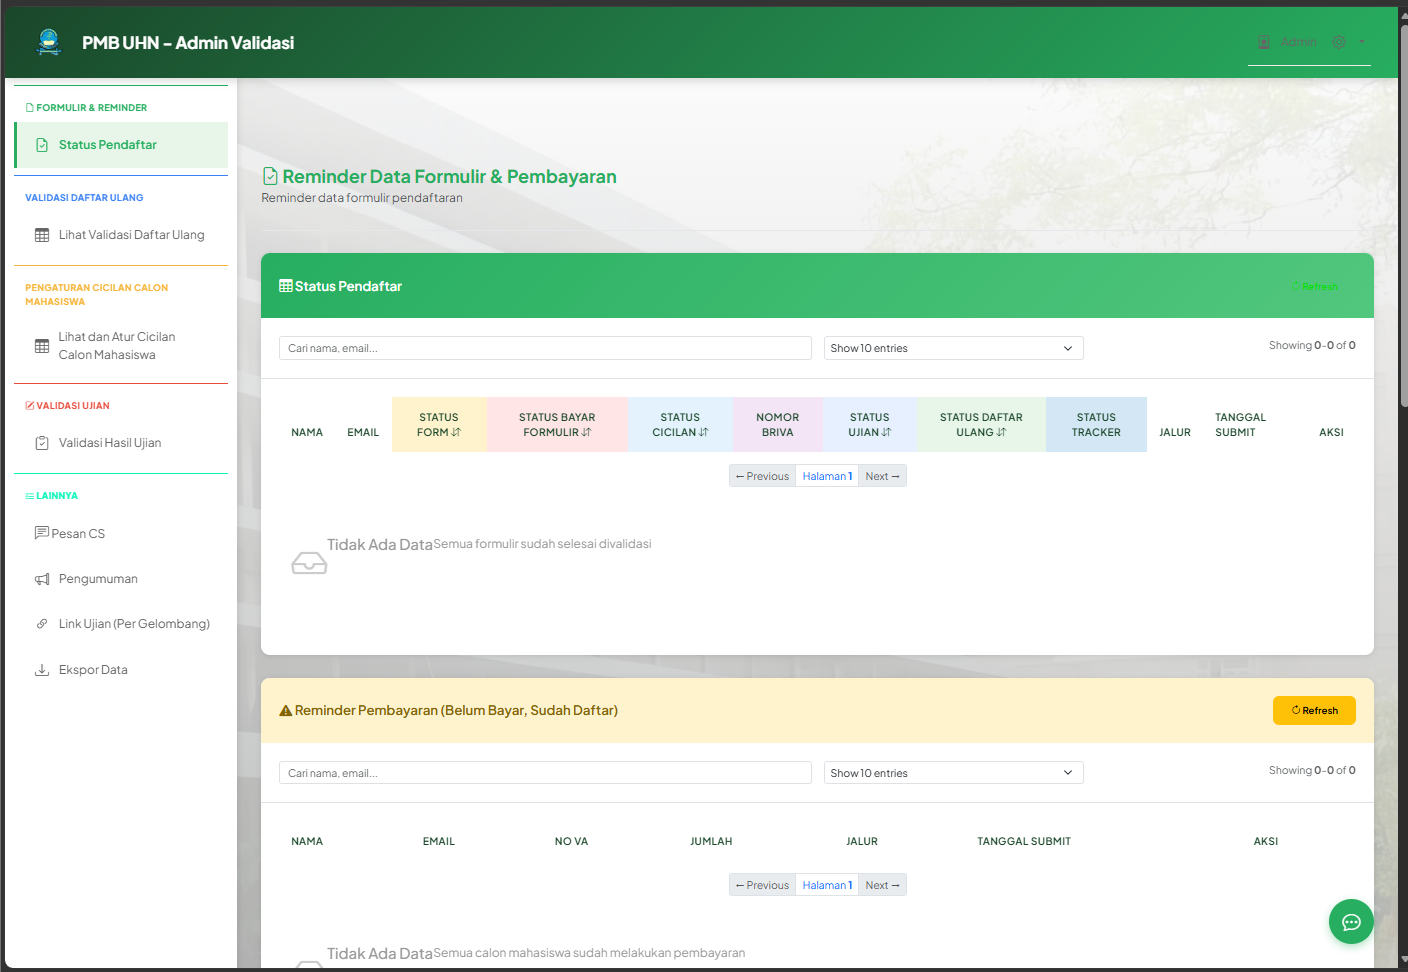
\includegraphics[width=0.9\textwidth]{figure/bab4/m-admin-validasi.png}
	\caption{Panel Validasi Formulir di Dasbor Admin Validasi}
	\label{fig:4.admin_validasi}
\end{figure}

\begin{lstlisting}[language=Java, caption={Endpoint persetujuan formulir dan permintaan revisi oleh admin}, label={kode:4.admin_validasi}]
// AdminController.java
@PutMapping("/api/validasi/formulir/{validationId}/approve")
@PreAuthorize("hasAnyRole('ADMIN_VALIDASI', 'ADMIN_PUSAT')")
public ResponseEntity<?> approveFormulir(@PathVariable Long validationId,
        @RequestBody ApproveRequest req) {
    // Set status = APPROVED, kirim email, buka akses ujian
    return ResponseEntity.ok(validasiService.approve(validationId, req));
}
@PutMapping("/api/validasi/formulir/{validationId}/revision-needed")
@PreAuthorize("hasAnyRole('ADMIN_VALIDASI', 'ADMIN_PUSAT')")
public ResponseEntity<?> mintaRevisi(@PathVariable Long validationId,
        @RequestBody RevisionRequest req) {
    // Set status = REVISION_NEEDED, kirim email dengan catatan
    return ResponseEntity.ok(validasiService.requestRevision(validationId, req));
}
\end{lstlisting}

% ------------------------------------------------
\subsubsection{Modul 18 --- Manajemen Ujian (Admin)} \label{IV.Mod.AdminUjian}
% ------------------------------------------------

Admin dapat mengonfigurasi tautan ujian \textit{online}/\textit{offline} per gelombang, melihat daftar peserta yang telah mengumpulkan ujian, dan membuat token ujian untuk peserta tertentu. Pada prototipe awal, belum ada fitur penetapan status lulus/tidak lulus yang eksplisit (ditambahkan pada Iterasi 1). Tampilan manajemen ujian ditunjukkan pada Gambar \ref{fig:4.admin_ujian}.\par

\begin{figure}[H]
	\centering
	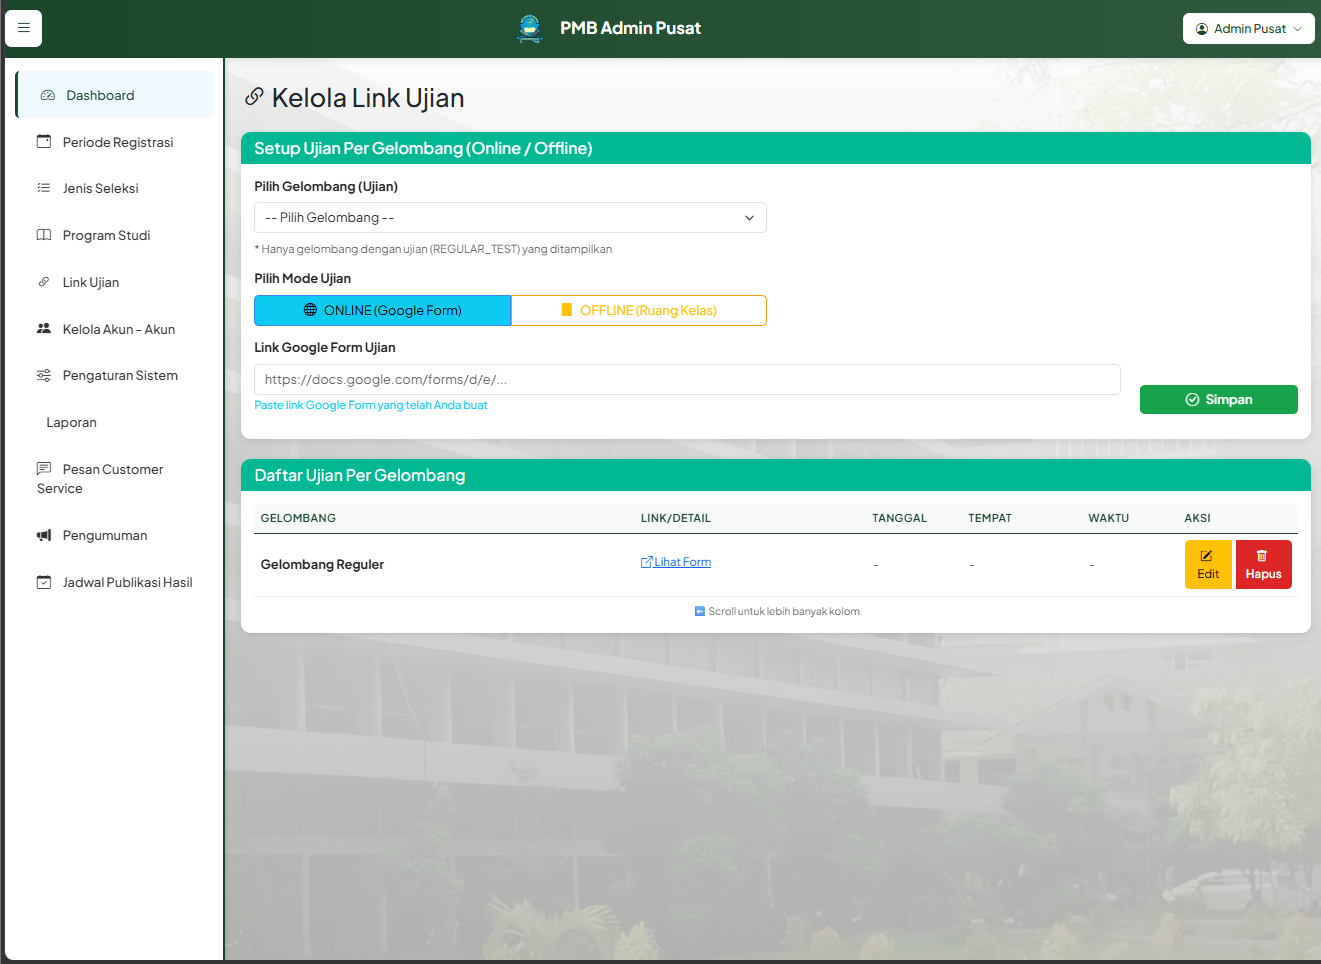
\includegraphics[width=0.9\textwidth]{figure/bab4/m-admin-ujian.png}
	\caption{Panel Manajemen Ujian dan Konfigurasi Link Ujian}
	\label{fig:4.admin_ujian}
\end{figure}

\begin{lstlisting}[language=Java, caption={Endpoint konfigurasi link ujian per gelombang dan daftar peserta ujian}, label={kode:4.admin_ujian}]
// AdminController.java
@PostMapping("/api/exam-links")
@PreAuthorize("hasRole('ADMIN_PUSAT')")
public ResponseEntity<?> setExamLink(@RequestBody ExamLinkRequest req) {
    // Simpan URL ujian online/offline per gelombang
    return ResponseEntity.ok(examLinkService.save(req));
}
@GetMapping("/exam-submissions")
@PreAuthorize("hasAnyRole('ADMIN_VALIDASI', 'ADMIN_PUSAT')")
public ResponseEntity<?> getExamSubmissions(
        @RequestParam(required = false) Long periodId) {
    // Kembalikan list exam_submissions beserta detail camaba
    return ResponseEntity.ok(examService.getSubmissions(periodId));
}
\end{lstlisting}

% ------------------------------------------------
\subsubsection{Modul 19 --- Validasi Daftar Ulang (Admin)} \label{IV.Mod.AdminDaftarUlang}
% ------------------------------------------------

Admin Validasi dapat melihat daftar proses daftar ulang yang masuk, memeriksa dokumen per dokumen, dan menyelesaikan proses validasi secara keseluruhan. Finalisasi daftar ulang memicu pembuatan rekaman Hasil Akhir untuk mahasiswa bersangkutan. Tampilan panel validasi daftar ulang ditunjukkan pada Gambar \ref{fig:4.admin_daftarulang}.\par

\begin{figure}[H]
	\centering
	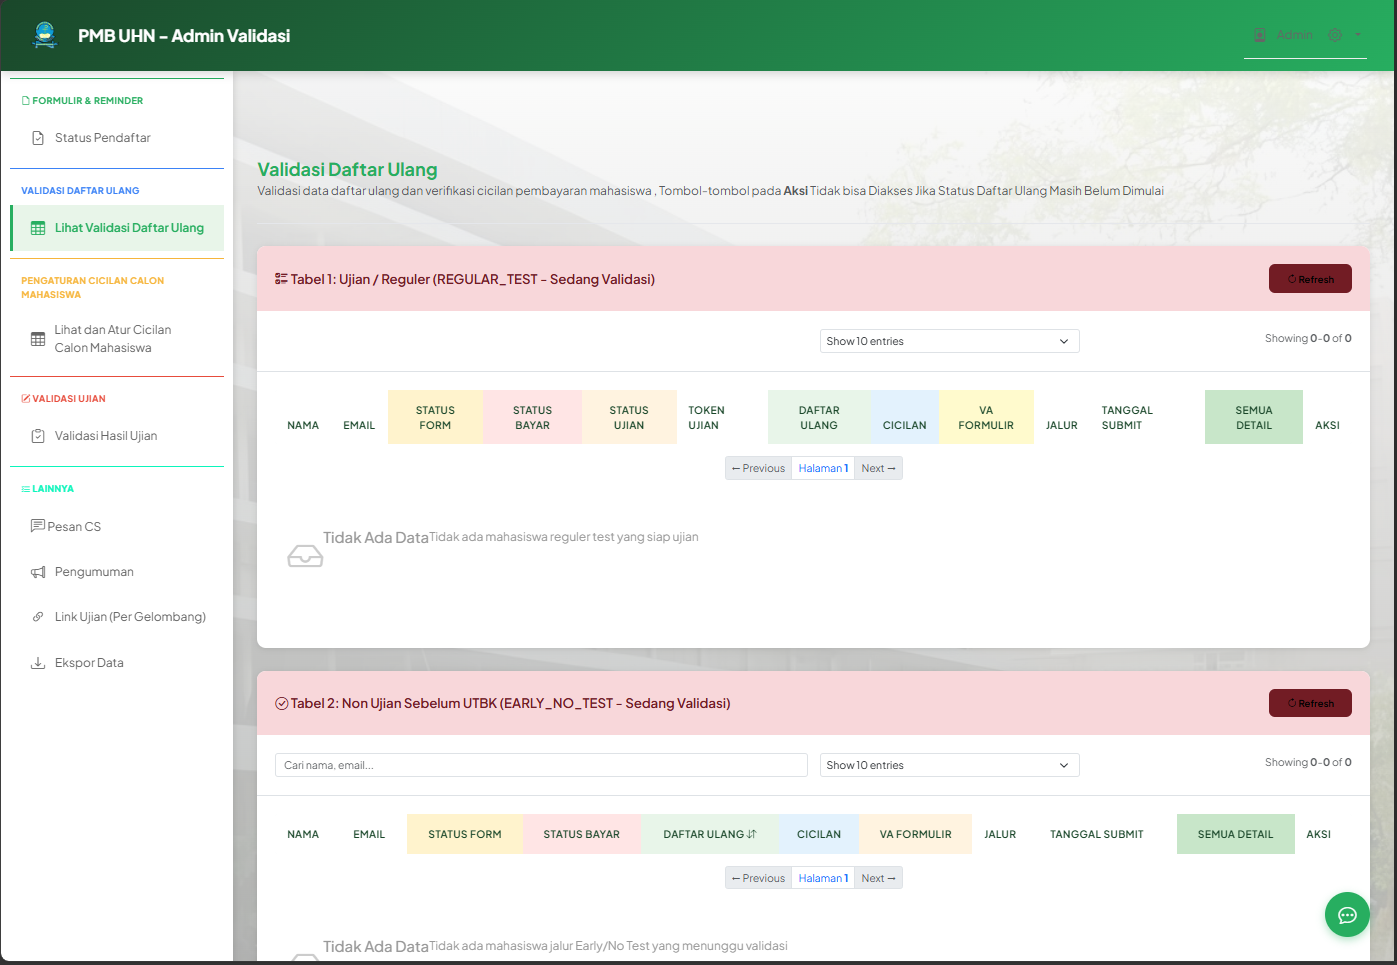
\includegraphics[width=0.9\textwidth]{figure/bab4/m-admin-daftar-ulang.png}
	\caption{Panel Validasi Daftar Ulang di Dasbor Admin Validasi}
	\label{fig:4.admin_daftarulang}
\end{figure}

\begin{lstlisting}[language=Java, caption={Endpoint validasi dokumen daftar ulang dan finalisasi proses}, label={kode:4.admin_daftarulang}]
// AdminController.java
@PutMapping("/api/reenrollments/documents/{docId}/validate")
@PreAuthorize("hasAnyRole('ADMIN_VALIDASI', 'ADMIN_PUSAT')")
public ResponseEntity<?> validateDocument(@PathVariable Long docId,
        @RequestBody DocumentValidationRequest req) {
    // Tandai dokumen sebagai VALID atau INVALID beserta catatan
    return ResponseEntity.ok(reenrollService.validateDoc(docId, req));
}
@PutMapping("/api/reenrollments/{id}/finalize")
@PreAuthorize("hasAnyRole('ADMIN_VALIDASI', 'ADMIN_PUSAT')")
public ResponseEntity<?> finalizeReenrollment(@PathVariable Long id) {
    // Tandai re_enrollment COMPLETE, buat rekaman HasilAkhir
    return ResponseEntity.ok(reenrollService.finalize(id));
}
\end{lstlisting}

% ------------------------------------------------
\subsubsection{Modul 20 --- Manajemen Cicilan (Admin)} \label{IV.Mod.AdminCicilan}
% ------------------------------------------------

Admin dapat melihat daftar pengajuan cicilan yang menunggu persetujuan, menyetujui atau menolak pengajuan, dan memantau status pembayaran setiap tahap cicilan. Persetujuan memicu pengiriman email notifikasi ke camaba. Tampilan panel manajemen cicilan ditunjukkan pada Gambar \ref{fig:4.admin_cicilan}.\par

\begin{figure}[H]
	\centering
	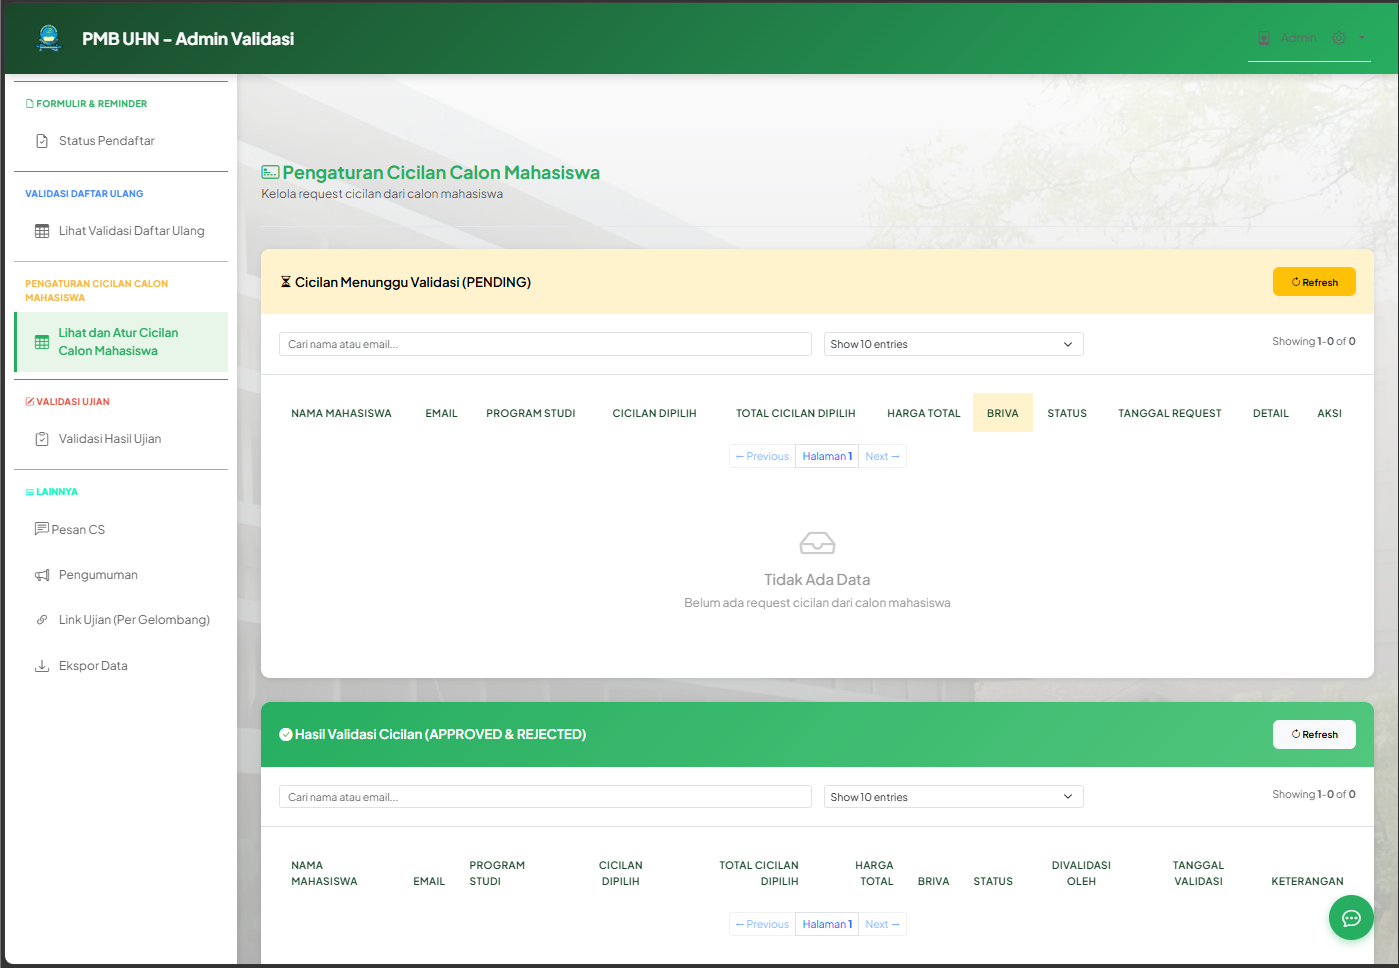
\includegraphics[width=0.9\textwidth]{figure/bab4/m-admin-cicilan.png}
	\caption{Panel Manajemen Cicilan di Dasbor Admin}
	\label{fig:4.admin_cicilan}
\end{figure}

\begin{lstlisting}[language=Java, caption={Endpoint approve dan reject cicilan di AdminCicilanController}, label={kode:4.admin_cicilan}]
// AdminCicilanController.java  -- prefix: /admin/cicilan
@GetMapping("/pending")
@PreAuthorize("hasAnyRole('ADMIN_PUSAT', 'ADMIN_VALIDASI')")
public ResponseEntity<?> getPendingCicilan() {
    return ResponseEntity.ok(cicilanRepo
        .findByStatus(CicilanRequestStatus.PENDING));
}
@PostMapping("/approve-installment")
@PreAuthorize("hasAnyRole('ADMIN_PUSAT', 'ADMIN_VALIDASI')")
public ResponseEntity<?> approveCicilan(@RequestBody ApproveRequest req) {
    // Set status = APPROVED
    // Generate jadwal cicilan berdasarkan skema yang dipilih
    // Kirim email notifikasi ke camaba
    return ResponseEntity.ok(cicilanService.approve(req));
}
\end{lstlisting}

% ------------------------------------------------
\subsubsection{Modul 21 --- Manajemen Pengumuman (Admin)} \label{IV.Mod.AdminPengumuman}
% ------------------------------------------------

Admin Pusat dapat membuat, memperbarui, menonaktifkan, dan menghapus pengumuman yang ditampilkan kepada camaba. Setiap pengumuman memiliki kategori, tingkat urgensi, dan tanggal kedaluwarsa. Tampilan manajemen pengumuman ditunjukkan pada Gambar \ref{fig:4.admin_pengumuman}.\par

\begin{figure}[H]
	\centering
	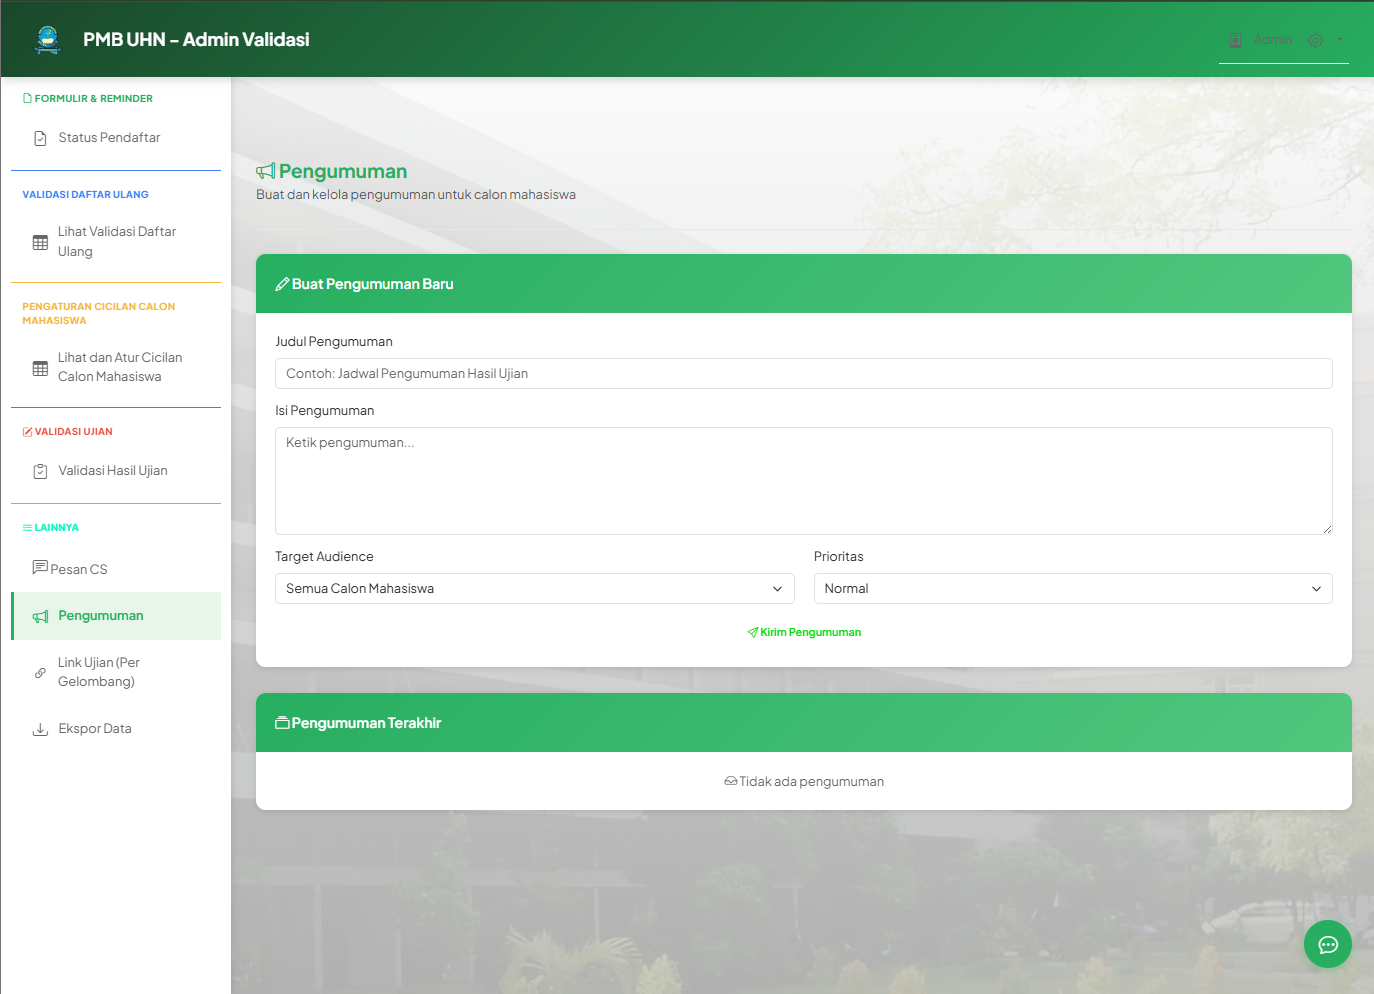
\includegraphics[width=0.9\textwidth]{figure/bab4/m-admin-pengumuman.png}
	\caption{Halaman Manajemen Pengumuman di Dasbor Admin Pusat}
	\label{fig:4.admin_pengumuman}
\end{figure}

\begin{lstlisting}[language=Java, caption={Endpoint CRUD pengumuman di AdminController}, label={kode:4.admin_pengumuman}]
// AdminController.java
@PostMapping("/api/announcements")
@PreAuthorize("hasRole('ADMIN_PUSAT')")
public ResponseEntity<?> createAnnouncement(
        @RequestBody AnnouncementRequest req) {
    // Simpan ke tabel announcements; isActive = true
    return ResponseEntity.ok(announcementService.create(req));
}
@GetMapping("/api/announcements/recent")
@PreAuthorize("hasAnyRole('ADMIN_PUSAT', 'ADMIN_VALIDASI')")
public ResponseEntity<?> getRecentAnnouncements() {
    // Kembalikan 5 pengumuman terbaru yang masih aktif
    return ResponseEntity.ok(announcementService.getRecent(5));
}
\end{lstlisting}

% ------------------------------------------------
\subsubsection{Modul 22 --- Manajemen Pengguna (Admin)} \label{IV.Mod.AdminUsers}
% ------------------------------------------------

Admin Pusat dapat melihat daftar seluruh pengguna sistem, mengubah peran (\textit{role}) pengguna antara \texttt{ADMIN\_PUSAT}, \texttt{ADMIN\_VALIDASI}, dan \texttt{CAMABA}, serta menonaktifkan atau menghapus akun yang tidak diperlukan. Tampilan manajemen pengguna ditunjukkan pada Gambar \ref{fig:4.admin_users}.\par

\begin{figure}[H]
	\centering
	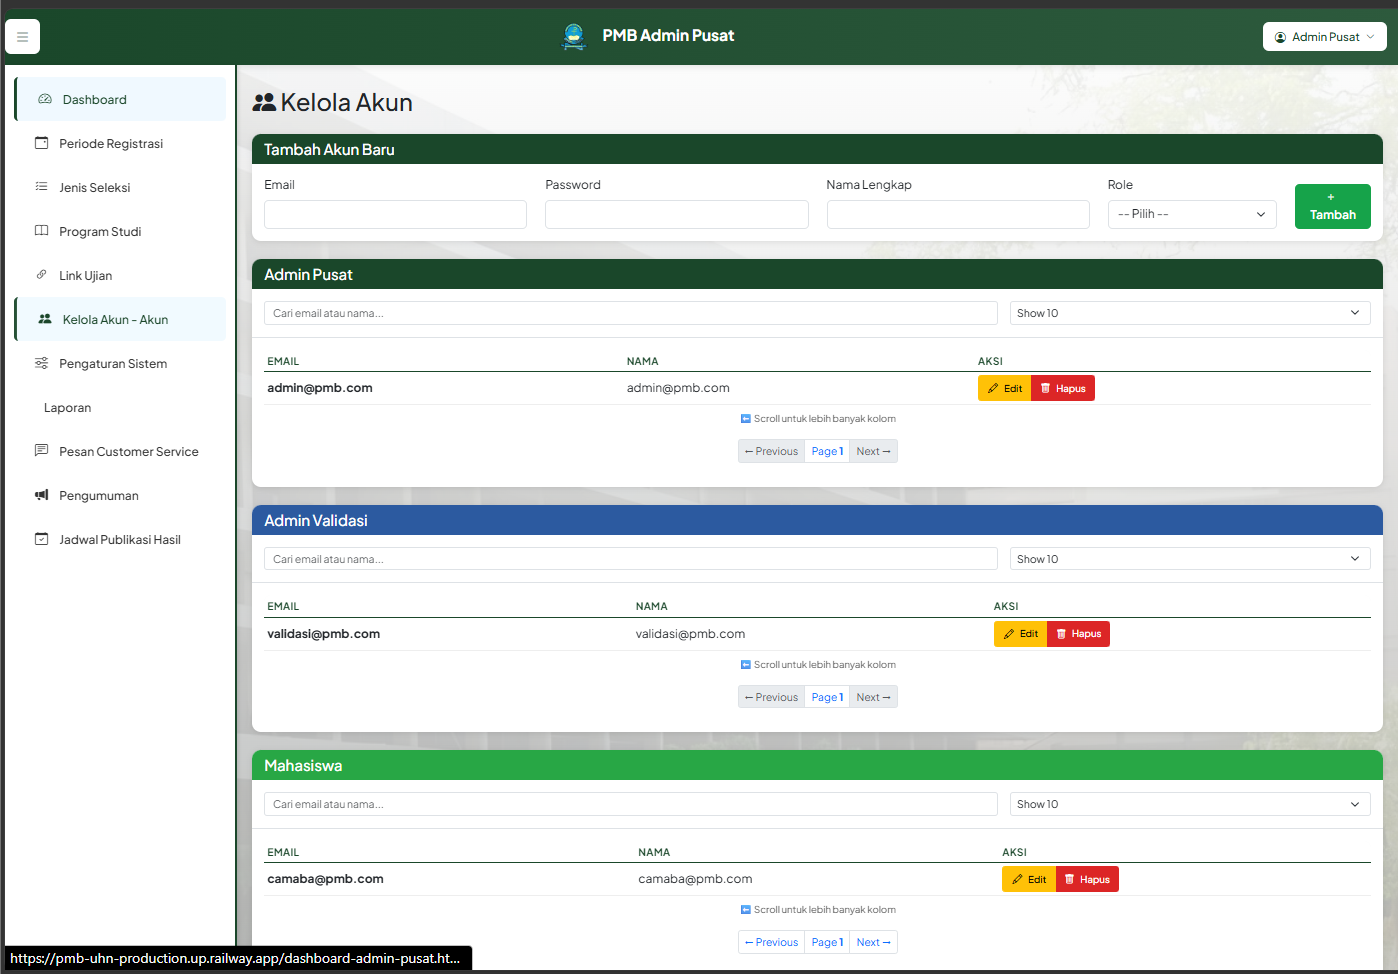
\includegraphics[width=0.9\textwidth]{figure/bab4/m-admin-users.png}
	\caption{Halaman Manajemen Pengguna di Dasbor Admin Pusat}
	\label{fig:4.admin_users}
\end{figure}

\begin{lstlisting}[language=Java, caption={Endpoint manajemen pengguna: daftar, ubah role, dan hapus akun}, label={kode:4.admin_users}]
// AdminController.java
@GetMapping("/api/users")
@PreAuthorize("hasRole('ADMIN_PUSAT')")
public ResponseEntity<?> getAllUsers(
        @RequestParam(required = false) String role) {
    // Filter berdasarkan role jika parameter disediakan
    return ResponseEntity.ok(userService.getAll(role));
}
@PutMapping("/api/users/{id}/role")
@PreAuthorize("hasRole('ADMIN_PUSAT')")
public ResponseEntity<?> changeUserRole(@PathVariable Long id,
        @RequestBody RoleChangeRequest req) {
    // Validasi: tidak boleh mengubah role diri sendiri
    return ResponseEntity.ok(userService.changeRole(id, req.getRole()));
}
\end{lstlisting}

% ============================================================
\subsection{Evaluasi dan Perbaikan} \label{IV.EvaluasiPerbaikan}
% ============================================================

Setelah prototipe awal selesai diimplementasikan, dilakukan serangkaian evaluasi melalui pengujian fungsional oleh tim pengembang dan demonstrasi langsung kepada pihak klien (Pusat Sistem Informasi UHN). Evaluasi ini menghasilkan temuan yang dikategorikan ke dalam iterasi-iterasi perbaikan. Subbab berikut merangkum hasil setiap iterasi.\par

% ------------------------------------------------
\subsubsection{Iterasi 1} \label{IV.Evaluasi.Iterasi1}
% ------------------------------------------------

Iterasi 1 mencakup sepuluh item perbaikan dan penambahan fitur: empat modul baru yang teridentifikasi dari evaluasi internal (\textbf{A7} Manajemen \textit{System Links}, \textbf{A8} Manajemen Informasi Kontak, \textbf{A14} Halaman Ekspor Data, \textbf{A17} \textit{Customer Service Chat Widget}), serta enam peningkatan pada modul yang ada berdasarkan umpan balik klien (verifikasi email, \textit{autocomplete} SMA, validasi kelulusan ujian, cicilan fleksibel, harga cicilan per program studi, dan cetak dokumen sementara).\par

\paragraph{A.\ Verifikasi Email pada Registrasi}

Pihak klien meminta agar sistem memverifikasi keabsahan alamat email yang didaftarkan agar tidak ada akun fiktif. Setelah implementasi, proses registrasi mengirimkan email berisi tautan verifikasi unik; camaba baru dapat masuk ke sistem setelah mengklik tautan tersebut. Ditambahkan pula \textit{endpoint} \texttt{POST /api/auth/resend-verification} untuk pengiriman ulang apabila token kedaluwarsa.\par

\noindent\textbf{Sebelum Iterasi 1:} Akun langsung diaktifkan sesaat setelah registrasi tanpa verifikasi email. Potongan kode sebelum perbaikan ditunjukkan pada Kode \ref{kode:4.iter1.verif.before}.\par

\begin{lstlisting}[language=Java, caption={Registrasi prototipe awal --- akun diaktifkan langsung}, label={kode:4.iter1.verif.before}]
// AuthController.java -- sebelum Iterasi 1
@PostMapping("/register")
public ResponseEntity<?> register(@RequestBody RegisterRequest req) {
    User user = User.builder()
        .email(req.getEmail())
        .password(encoder.encode(req.getPassword()))
        .nama(req.getNama())
        .enabled(true)          // langsung aktif, tanpa cek email
        .build();
    userRepo.save(user);
    return ResponseEntity.ok(Map.of("message", "Registrasi berhasil"));
}
\end{lstlisting}

\noindent\textbf{Setelah Iterasi 1:} Registrasi mengirim email verifikasi; akun hanya aktif setelah tautan diklik. Tersedia juga \textit{endpoint} kirim ulang token. Tampilan dan kode setelah perbaikan ditunjukkan pada Gambar \ref{fig:4.iter1.verif.after} dan Kode \ref{kode:4.iter1.verif}.\par

\begin{figure}[H]
	\centering
	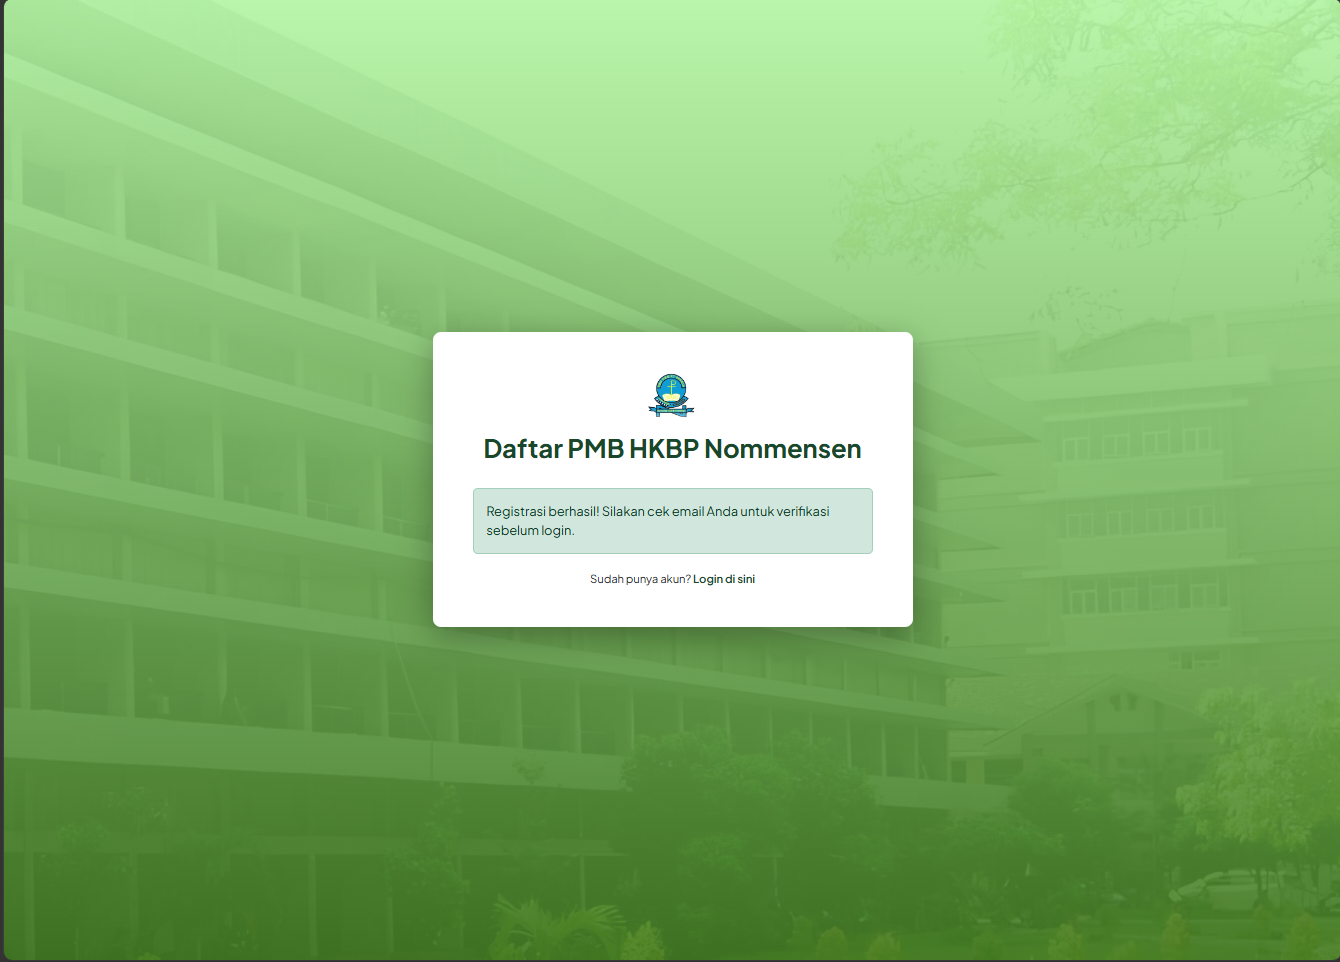
\includegraphics[width=0.75\textwidth]{figure/bab4/iter1-verif-after.png}
	\caption{Notifikasi Verifikasi Email setelah Iterasi 1 --- Camaba Harus Klik Tautan Sebelum Login}
	\label{fig:4.iter1.verif.after}
\end{figure}

\begin{lstlisting}[language=Java, caption={Endpoint verifikasi email dan pengiriman ulang di AuthController}, label={kode:4.iter1.verif}]
// AuthController.java  -- /api/auth/**  (permitAll)
@GetMapping("/verify-email")
public ResponseEntity<?> verifyEmail(@RequestParam String token) {
    // Cari token di email_verification_tokens, cek expiry
    // Set emailVerified = true, invalidasi token
    return ResponseEntity.ok(authService.verifyEmail(token));
}
@PostMapping("/resend-verification")
public ResponseEntity<?> resendVerification(
        @RequestBody ResendVerifRequest req) {
    // Buat token baru, kirim ulang email verifikasi
    return ResponseEntity.ok(authService.resendVerification(req.getEmail()));
}
\end{lstlisting}

\paragraph{B.\ \textit{Autocomplete} Asal Sekolah}

Kolom asal sekolah pada formulir pendaftaran ditingkatkan dengan \textit{dropdown} pencarian. Pengguna mengetik minimal dua karakter, sistem mencari ke basis data sekolah dan menampilkan saran dengan \textit{debouncing} 300 ms. Jika sekolah tidak ditemukan, tersedia opsi input manual yang disimpan di kolom \texttt{sekolah\_manual}.\par

\noindent\textbf{Sebelum Iterasi 1:} Kolom asal sekolah berupa \textit{input} teks bebas tanpa bantuan pencarian. Potongan kode sebelum perbaikan ditunjukkan pada Kode \ref{kode:4.iter1.autocomplete.before}.\par

\begin{lstlisting}[language=Java, caption={Entitas AdmissionForm prototipe awal --- kolom asal sekolah teks bebas}, label={kode:4.iter1.autocomplete.before}]
// AdmissionForm.java -- sebelum Iterasi 1
@Column(name = "asal_sekolah")
private String asalSekolah;  // input teks bebas, tidak ada validasi
// Tidak ada endpoint pencarian sekolah; kolom sekolah_manual belum ada
\end{lstlisting}

\noindent\textbf{Setelah Iterasi 1:} Kolom dilengkapi \textit{dropdown} pencarian dengan \textit{debouncing}; input manual tersimpan di kolom cadangan. Tampilan dan kode setelah perbaikan ditunjukkan pada Gambar \ref{fig:4.iter1.autocomplete.after} dan Kode \ref{kode:4.iter1.autocomplete}.\par

\begin{figure}[H]
	\centering
	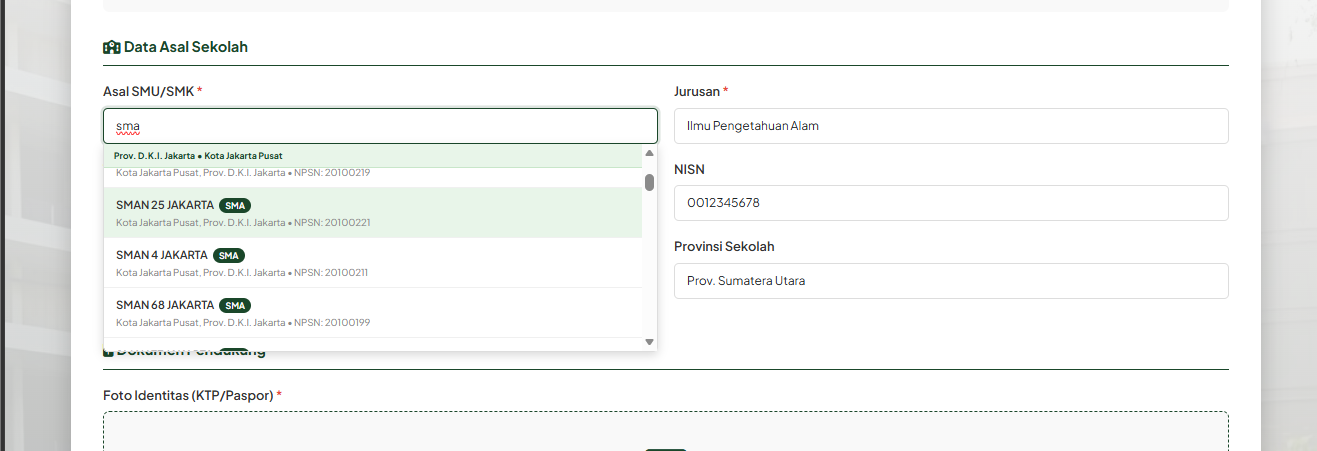
\includegraphics[width=0.85\textwidth]{figure/bab4/iter1-autocomplete-after.png}
	\caption{Formulir Pendaftaran setelah Iterasi 1 --- Kolom Asal Sekolah dengan \textit{Autocomplete}}
	\label{fig:4.iter1.autocomplete.after}
\end{figure}

\begin{lstlisting}[language=Java, caption={Endpoint autocomplete pencarian sekolah di PublicApiController}, label={kode:4.iter1.autocomplete}]
// PublicApiController.java  -- /api/public/**  (permitAll)
@GetMapping("/sekolah/search")
public ResponseEntity<?> searchSekolah(@RequestParam String q) {
    // LIKE '%q%' pada nama sekolah, batas 10 hasil
    return ResponseEntity.ok(sekolahRepo
        .findByNamaContainingIgnoreCase(q, PageRequest.of(0, 10)));
}
\end{lstlisting}

\paragraph{C.\ Validasi Kelulusan Ujian}

Ditambahkan mekanisme eksplisit bagi Admin Validasi untuk menetapkan status lulus atau tidak lulus ujian. Penetapan ini memicu notifikasi email ke camaba dan mengontrol akses ke tahap daftar ulang.\par

\noindent\textbf{Sebelum Iterasi 1:} Admin hanya dapat melihat daftar pengumpulan ujian; tidak ada tombol penetapan lulus/tidak lulus. Potongan kode sebelum perbaikan ditunjukkan pada Kode \ref{kode:4.iter1.lulusujian.before}.\par

\begin{lstlisting}[language=Java, caption={AdminController prototipe awal --- hanya menampilkan daftar ujian}, label={kode:4.iter1.lulusujian.before}]
// AdminController.java -- sebelum Iterasi 1
// Hanya menampilkan daftar pengumpulan; tidak ada endpoint validasi kelulusan
@GetMapping("/exam-submissions")
@PreAuthorize("hasAnyRole('ADMIN_VALIDASI', 'ADMIN_PUSAT')")
public ResponseEntity<?> getExamSubmissions(
        @RequestParam(required = false) Long gelombangId) {
    return ResponseEntity.ok(examSubmissionRepo.findAll());
}
\end{lstlisting}

\noindent\textbf{Setelah Iterasi 1:} Ditambahkan tombol validasi lulus/tidak lulus yang memicu notifikasi email dan membuka akses daftar ulang. Tampilan dan kode setelah perbaikan ditunjukkan pada Gambar \ref{fig:4.iter1.lulusujian.after} dan Kode \ref{kode:4.iter1.lulusujian}.\par

\begin{figure}[H]
	\centering
	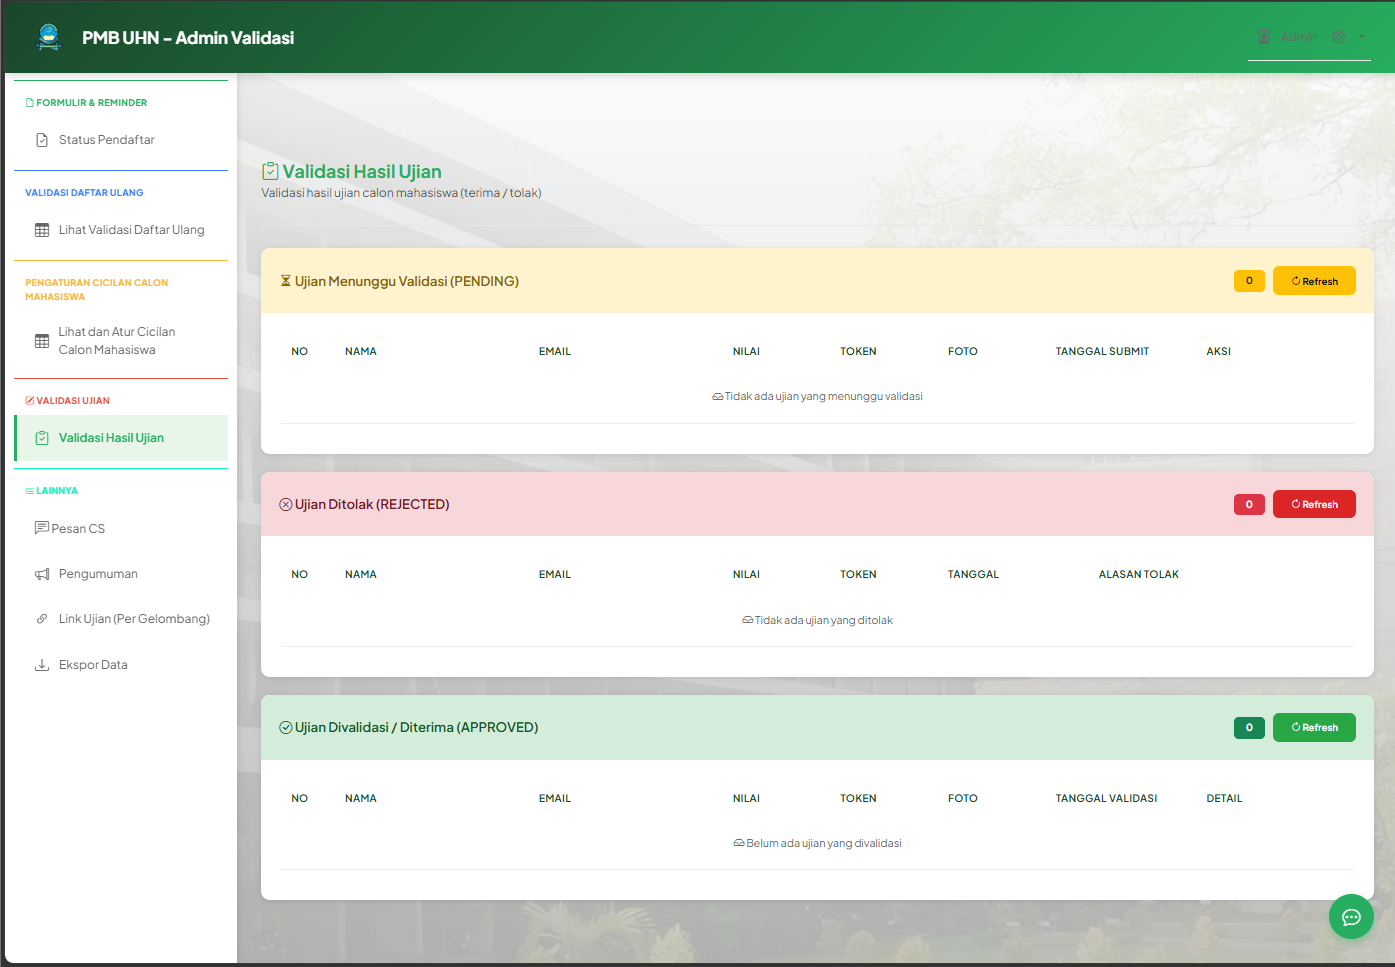
\includegraphics[width=0.9\textwidth]{figure/bab4/iter1-lulusujian-after.png}
	\caption{Halaman Manajemen Ujian setelah Iterasi 1 --- Tombol Validasi Kelulusan Aktif}
	\label{fig:4.iter1.lulusujian.after}
\end{figure}

\begin{lstlisting}[language=Java, caption={Endpoint validasi kelulusan ujian oleh admin}, label={kode:4.iter1.lulusujian}]
// AdminController.java
@PostMapping("/exam-submissions/{id}/validate")
@PreAuthorize("hasAnyRole('ADMIN_VALIDASI', 'ADMIN_PUSAT')")
public ResponseEntity<?> validateExam(@PathVariable Long id,
        @RequestBody ExamValidationRequest req) {
    // req.result = LULUS | TIDAK_LULUS; req.catatan (opsional)
    // Jika LULUS: buka akses daftar ulang; Jika TIDAK_LULUS: tutup akses
    // Kirim email notifikasi ke camaba
    return ResponseEntity.ok(examService.validate(id, req));
}
\end{lstlisting}

\paragraph{D.\ Cicilan Fleksibel}

Cicilan ditingkatkan dari permintaan sederhana menjadi skema terstruktur. Camaba kini dapat memilih jumlah cicilan (1\texttimes{} hingga 6\texttimes{}); sistem secara otomatis menghasilkan jadwal cicilan berdasarkan harga per-tahap yang dikonfigurasi admin. Selisih pembulatan diserap oleh cicilan terakhir.\par

\noindent\textbf{Sebelum Iterasi 1:} Cicilan hanya berupa pengajuan sederhana tanpa konfigurasi jumlah tahap; skema ditentukan admin secara manual. Potongan kode sebelum perbaikan ditunjukkan pada Kode \ref{kode:4.iter1.cicilan.before}.\par

\begin{lstlisting}[language=Java, caption={CicilanRequestController prototipe awal --- pengajuan sederhana tanpa tahap}, label={kode:4.iter1.cicilan.before}]
// CicilanRequestController.java -- sebelum Iterasi 1
@PostMapping("/submit")
public ResponseEntity<?> submitCicilan(
        @RequestBody CicilanSimpleRequest req, Principal principal) {
    // Hanya menyimpan pengajuan; jumlah cicilan ditentukan admin secara manual
    CicilanEntry cicilan = new CicilanEntry();
    cicilan.setStudentId(getStudentId(principal));
    cicilan.setKeterangan(req.getKeterangan());
    cicilan.setStatus("PENDING");
    return ResponseEntity.ok(cicilanRepo.save(cicilan));
}
\end{lstlisting}

\noindent\textbf{Setelah Iterasi 1:} Camaba memilih jumlah tahap (1--6\texttimes{}); jadwal cicilan dibuat otomatis dari harga per-tahap. Tampilan dan kode setelah perbaikan ditunjukkan pada Gambar \ref{fig:4.iter1.cicilan.after} dan Kode \ref{kode:4.iter1.cicilan}.\par

\begin{figure}[H]
	\centering
	\includegraphics[width=0.75\textwidth]{figure/bab4/iter1-cicilan-after.png}
	\caption{Halaman Pengajuan Cicilan setelah Iterasi 1 --- Pilihan Jumlah Tahap Cicilan}
	\label{fig:4.iter1.cicilan.after}
\end{figure}

\begin{lstlisting}[language=Java, caption={Pengajuan cicilan dengan pilihan jumlah tahap di CicilanRequestController}, label={kode:4.iter1.cicilan}]
// CicilanRequestController.java  -- POST /api/cicilan/submit
@PostMapping("/submit")
public ResponseEntity<?> submitCicilan(
        @RequestBody CicilanRequest req, Principal principal) {
    // req.jumlahCicilan = 1..6
    // Validasi: pembayaran belum verified, belum ada cicilan aktif
    // Generate jadwal dari harga_cicilan_1..N di ProgramStudi
    return ResponseEntity.ok(cicilanService.submit(req, principal));
}
\end{lstlisting}

\paragraph{E.\ Harga Cicilan per Program Studi}

Admin Pusat dapat mengonfigurasi nominal setiap tahap cicilan (Cicilan 1 s.d. Cicilan 6) untuk setiap program studi secara independen, dengan fitur \textit{auto-split} dan salin konfigurasi antar program studi.\par

\noindent\textbf{Sebelum Iterasi 1:} Entitas \texttt{ProgramStudi} hanya menyimpan \texttt{hargaTotal}; tidak ada kolom harga per tahap cicilan. Potongan kode sebelum perbaikan ditunjukkan pada Kode \ref{kode:4.iter1.hargacicilan.before}.\par

\begin{lstlisting}[language=Java, caption={Entitas ProgramStudi prototipe awal --- hanya hargaTotal}, label={kode:4.iter1.hargacicilan.before}]
// ProgramStudi.java -- sebelum Iterasi 1
@Column(name = "harga_total")
private Long hargaTotal;
// Kolom hargaCicilan1 s.d. hargaCicilan6 belum tersedia;
// skema cicilan dihitung manual oleh admin tanpa referensi harga tahap
\end{lstlisting}

\noindent\textbf{Setelah Iterasi 1:} Enam kolom harga cicilan ditambahkan; fitur \textit{auto-split} dan salin antar prodi tersedia. Tampilan dan kode setelah perbaikan ditunjukkan pada Gambar \ref{fig:4.iter1.hargacicilan.after} dan Kode \ref{kode:4.iter1.hargacicilan}.\par

\begin{figure}[H]
	\centering
	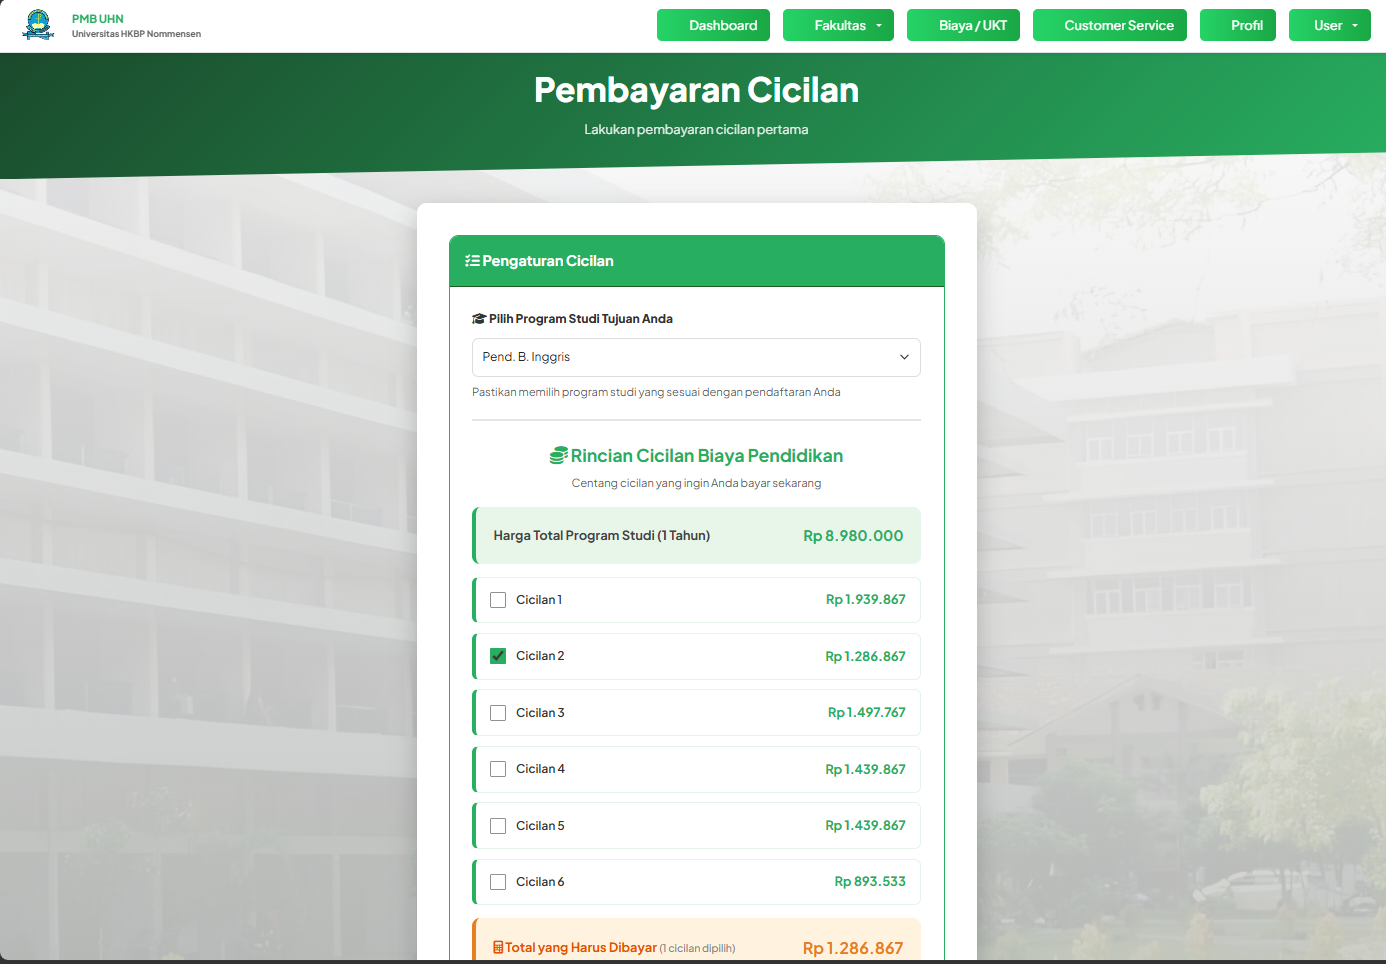
\includegraphics[width=0.9\textwidth]{figure/bab4/iter1-hargacicilan-after.png}
	\caption{Halaman Edit Program Studi setelah Iterasi 1 --- Harga per Tahap Cicilan Dapat Dikonfigurasi}
	\label{fig:4.iter1.hargacicilan.after}
\end{figure}

\begin{lstlisting}[language=Java, caption={Endpoint konfigurasi harga cicilan per program studi}, label={kode:4.iter1.hargacicilan}]
// AdminController.java
@PutMapping("/program-studi/{id}")
@PreAuthorize("hasRole('ADMIN_PUSAT')")
public ResponseEntity<?> updateProgramStudi(@PathVariable Long id,
        @RequestBody ProgramStudiRequest req) {
    // req berisi hargaCicilan1..6, auto-split dari hargaTotal
    // Validasi: total cicilan tidak melebihi hargaTotal
    return ResponseEntity.ok(programStudiService.update(id, req));
}
\end{lstlisting}

\paragraph{F.\ Cetak Dokumen Sementara}

Admin Validasi dapat mengunggah NPM Sementara dan KTM Sementara untuk mahasiswa yang telah selesai daftar ulang. Berkas disimpan di direktori \texttt{uploads/hasil-akhir/\{studentId\}/} dan disajikan melalui \texttt{FileServingController} yang mendukung mode tampil (\textit{inline}) dan unduh (\texttt{?download=true}).\par

\noindent\textbf{Sebelum Iterasi 1:} Modal Hasil Akhir hanya menampilkan nomor registrasi; tidak ada fitur unggah atau unduh dokumen sementara. Potongan kode sebelum perbaikan ditunjukkan pada Kode \ref{kode:4.iter1.dokumen.before}.\par

\begin{lstlisting}[language=Java, caption={Entitas HasilAkhir prototipe awal --- tanpa kolom file dokumen sementara}, label={kode:4.iter1.dokumen.before}]
// HasilAkhir.java -- sebelum Iterasi 1
@Column(name = "nomor_registrasi", unique = true)
private String nomorRegistrasi;
// Kolom npmSementaraFile dan ktmSementaraFile belum tersedia;
// tidak ada mekanisme unggah atau penyajian dokumen sementara
\end{lstlisting}

\noindent\textbf{Setelah Iterasi 1:} Dua kolom file ditambahkan ke entitas; admin dapat mengunggah dan camaba dapat mengunduh NPM/KTM Sementara. Tampilan dan kode setelah perbaikan ditunjukkan pada Gambar \ref{fig:4.iter1.dokumen.after} dan Kode \ref{kode:4.iter1.dokumen}.\par

\begin{figure}[H]
	\centering
	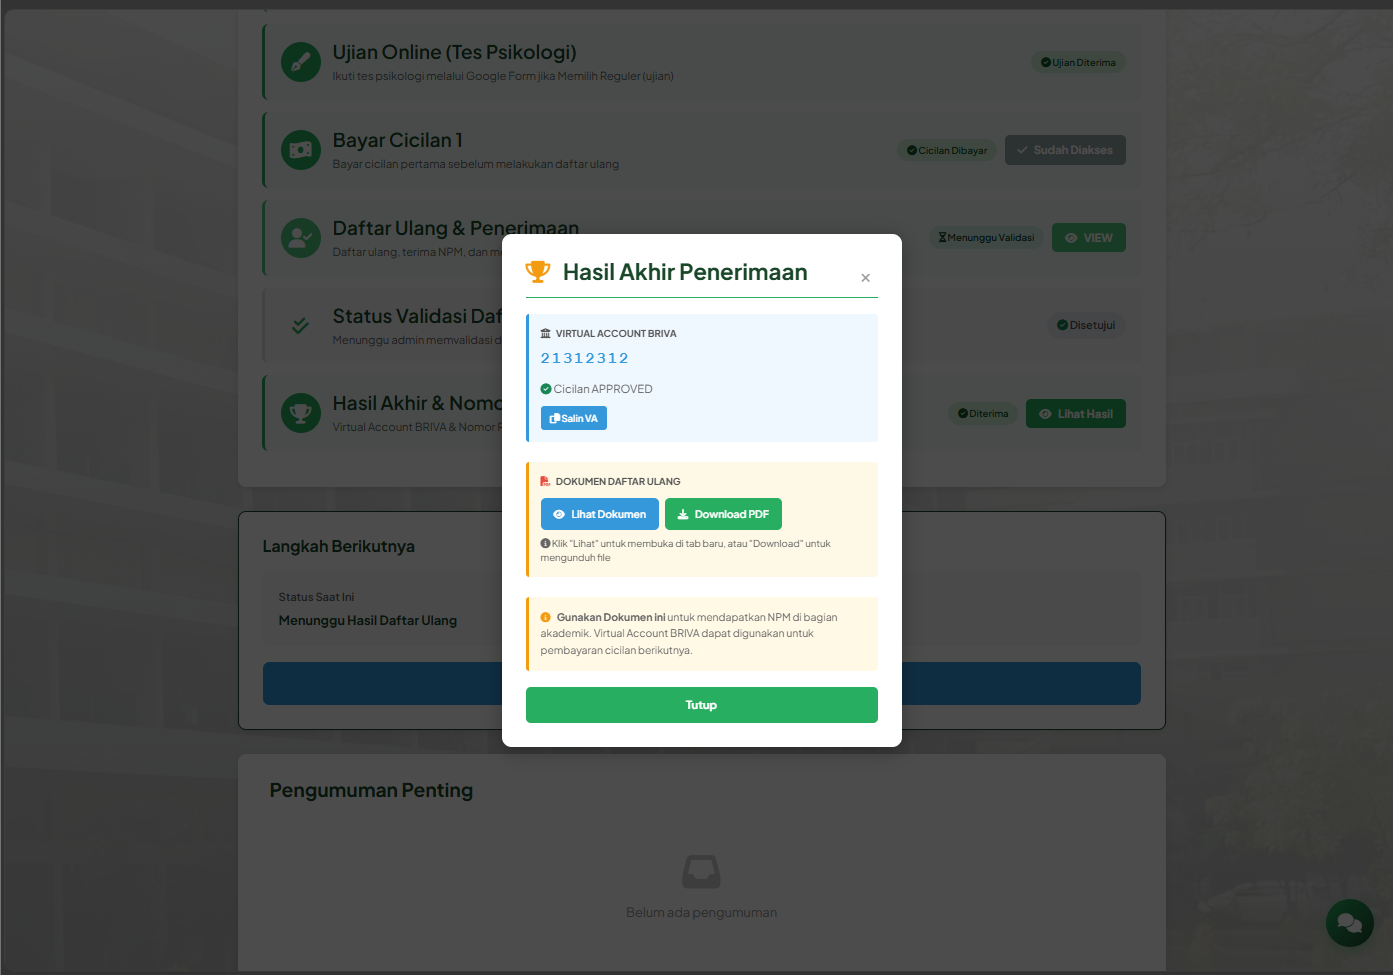
\includegraphics[width=0.8\textwidth]{figure/bab4/iter1-dokumen-after.png}
	\caption{Modal Hasil Akhir setelah Iterasi 1 --- Tombol Unduh NPM/KTM Sementara Tersedia}
	\label{fig:4.iter1.dokumen.after}
\end{figure}

\begin{lstlisting}[language=Java, caption={Endpoint upload dokumen sementara oleh admin dan penyajian file}, label={kode:4.iter1.dokumen}]
// AdminController.java
@PostMapping("/api/hasil-akhir/{id}/upload-dokumen")
@PreAuthorize("hasAnyRole('ADMIN_VALIDASI', 'ADMIN_PUSAT')")
public ResponseEntity<?> uploadDokumenSementara(
        @PathVariable Long id,
        @RequestParam(required = false) MultipartFile npmFile,
        @RequestParam(required = false) MultipartFile ktmFile) {
    HasilAkhir ha = hasilAkhirRepo.findById(id).orElseThrow();
    if (npmFile != null)
        ha.setNpmSementaraFile(fileStorage.save(npmFile,
            "hasil-akhir/" + ha.getStudent().getId()));
    if (ktmFile != null)
        ha.setKtmSementaraFile(fileStorage.save(ktmFile,
            "hasil-akhir/" + ha.getStudent().getId()));
    return ResponseEntity.ok(hasilAkhirRepo.save(ha));
}
// FileServingController.java -- GET /api/files/view/**
@GetMapping("/api/files/view/**")
public ResponseEntity<Resource> viewFile(HttpServletRequest request,
        @RequestParam(value = "download", defaultValue = "false")
        boolean download) {
    Resource res = fileStorage.loadAsResource(extractPath(request));
    return ResponseEntity.ok()
        .header(HttpHeaders.CONTENT_DISPOSITION,
            (download ? "attachment" : "inline")
            + "; filename=\"" + res.getFilename() + "\"")
        .body(res);
}
\end{lstlisting}

\paragraph{G.\ Manajemen \textit{System Links} dan Informasi Kontak (A7, A8)}

Admin Pusat dapat mengelola tautan eksternal (YouTube, Google Drive, Google Form, URL lainnya) serta informasi kontak institusi (alamat, telepon, email, jam layanan) melalui satu halaman pengaturan terpadu di dasbor admin. Kedua fitur ditampilkan secara dinamis di \textit{footer} halaman publik; tautan yang dikelola melalui \textit{System Links} menggunakan validasi format URL sebelum disimpan, sedangkan informasi kontak menggunakan pola \textit{singleton record}.\par

\noindent\textbf{Sebelum Iterasi 1:} Kedua modul belum tersedia. Seluruh tautan dan informasi kontak di-\textit{hardcode} di template HTML/Thymeleaf; perubahan memerlukan modifikasi kode dan redeployment.\par

\noindent\textbf{Setelah Iterasi 1:} Halaman pengaturan terpadu ditambahkan sehingga admin dapat mengelola \textit{system links} dan informasi kontak tanpa perlu menyentuh kode. Tampilan halaman ditunjukkan pada Gambar \ref{fig:4.iter1.syslinks} dan potongan kode kedua endpoint pada Kode \ref{kode:4.iter1.syslinks} dan Kode \ref{kode:4.iter1.kontak}.\par

\begin{figure}[H]
	\centering
	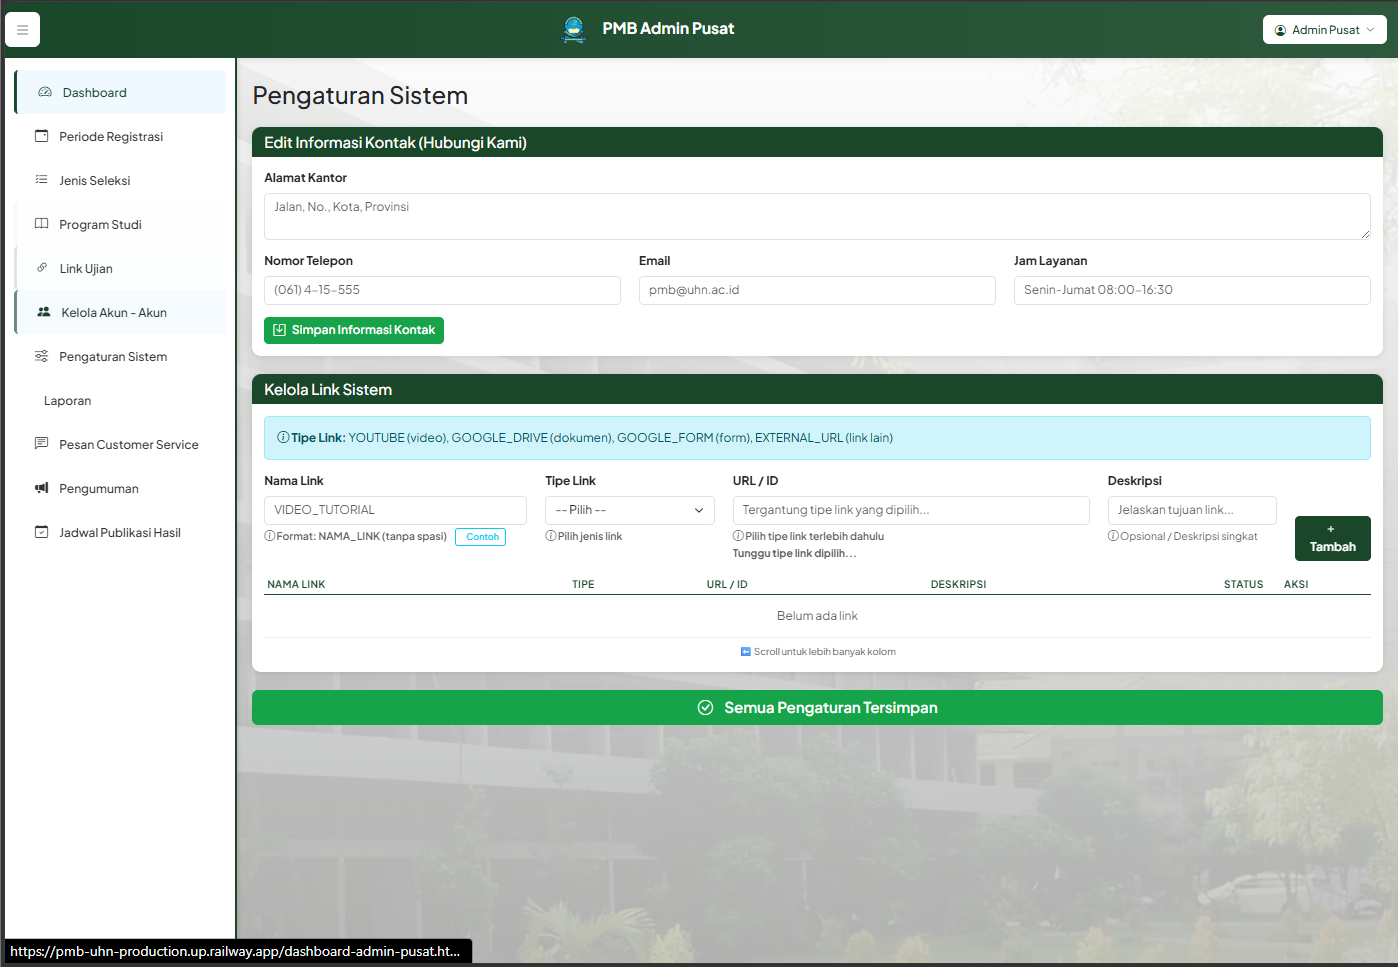
\includegraphics[width=0.9\textwidth]{figure/bab4/iter1-system-links.png}
	\caption{Halaman Manajemen \textit{System Links} dan Informasi Kontak di Dasbor Admin Pusat setelah Iterasi 1}
	\label{fig:4.iter1.syslinks}
\end{figure}

\begin{lstlisting}[language=Java, caption={Endpoint CRUD system links di SystemSettingsController}, label={kode:4.iter1.syslinks}]
// SystemSettingsController.java  -- prefix: /admin/api/system-settings
@PostMapping("/system-links")
@PreAuthorize("hasRole('ADMIN_PUSAT')")
public ResponseEntity<?> addLink(@RequestBody SystemLinkRequest req) {
    // Validasi format URL dengan regex sebelum disimpan
    return ResponseEntity.ok(systemLinkRepo.save(
        SystemLink.builder().nama(req.getNama()).tipe(req.getTipe())
            .url(req.getUrl()).isActive(true).build()));
}
// PublicSettingsController.java -- GET /api/public/settings/system-links
@GetMapping("/system-links")  // permitAll
public ResponseEntity<?> getActiveLinks() {
    return ResponseEntity.ok(systemLinkRepo.findByIsActiveTrue());
}
\end{lstlisting}

\begin{lstlisting}[language=Java, caption={Endpoint pembaruan informasi kontak dengan pola singleton record}, label={kode:4.iter1.kontak}]
// SystemSettingsController.java
@PostMapping("/contact-info")
@PreAuthorize("hasRole('ADMIN_PUSAT')")
public ResponseEntity<?> upsertContactInfo(
        @RequestBody ContactInfoRequest req) {
    // Pola singleton: findFirst(), jika tidak ada buat baru
    ContactInfo info = contactInfoRepo.findFirst().orElse(new ContactInfo());
    info.setAlamat(req.getAlamat()); info.setTelepon(req.getTelepon());
    info.setEmail(req.getEmail());  info.setJamLayanan(req.getJamLayanan());
    return ResponseEntity.ok(contactInfoRepo.save(info));
}
// PublicSettingsController.java -- GET /api/public/settings/contact-info
@GetMapping("/contact-info")  // permitAll
public ResponseEntity<?> getContactInfo() {
    return ResponseEntity.ok(contactInfoRepo.findFirst().orElse(null));
}
\end{lstlisting}

\paragraph{I.\ Halaman Ekspor Data (A14)}

Ditambahkan empat halaman ekspor terpisah: formulir pembayaran, data daftar ulang, hasil akhir, dan hasil akhir per gelombang. Setiap halaman memiliki panel filter dan \textit{preview} tabel (maksimal 100 baris) serta tombol ekspor dalam format CSV, JSON, dan Cetak.\par

\noindent\textbf{Sebelum Iterasi 1:} Tidak ada halaman ekspor di prototipe awal. Admin harus mengakses langsung konsol H2 atau mengekstrak data secara manual; tidak ada antarmuka terpadu untuk ekspor data.\par

\noindent\textbf{Setelah Iterasi 1:} Empat halaman ekspor dengan filter, preview, dan multi-format (CSV/JSON/Cetak) ditambahkan. Tampilan dan kode modul ditunjukkan pada Gambar \ref{fig:4.iter1.ekspor} dan Kode \ref{kode:4.iter1.ekspor}.\par

\begin{figure}[H]
	\centering
	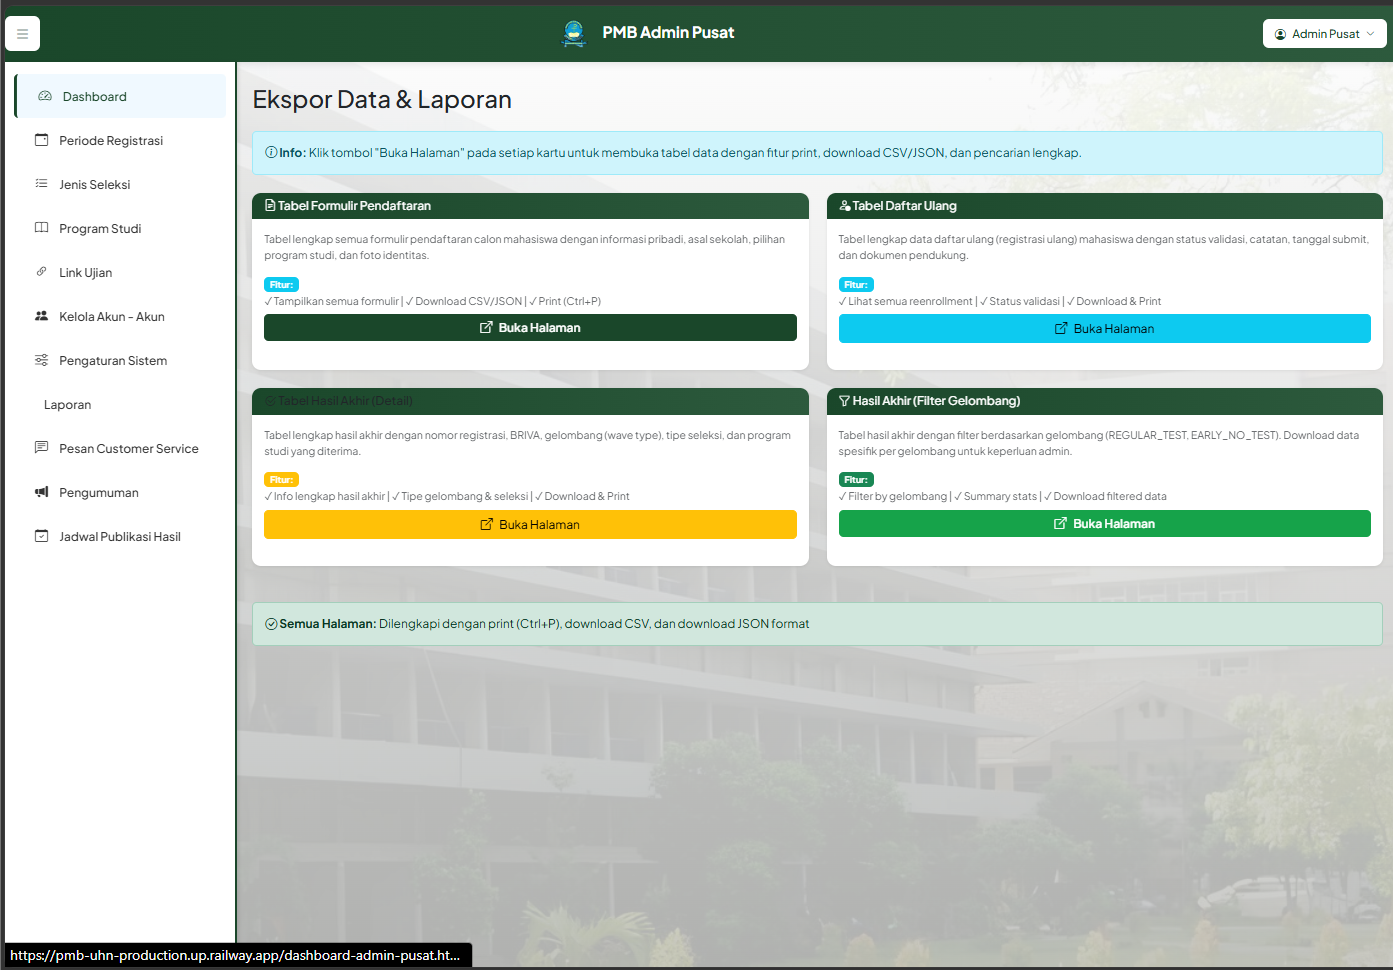
\includegraphics[width=0.9\textwidth]{figure/bab4/iter1-export.png}
	\caption{Halaman Ekspor Data Formulir Pendaftaran setelah Iterasi 1}
	\label{fig:4.iter1.ekspor}
\end{figure}

\begin{lstlisting}[language=Java, caption={Endpoint ekspor data formulir dalam format CSV dengan baris header}, label={kode:4.iter1.ekspor}]
// AdminController.java
@GetMapping("/api/export/formulir-pembayaran")
@PreAuthorize("hasAnyRole('ADMIN_PUSAT', 'ADMIN_VALIDASI')")
public ResponseEntity<String> exportFormulirCSV(
        @RequestParam(required = false) String gelombang,
        @RequestParam(required = false) String status) {
    List<AdmissionForm> data = formRepo.findWithFilter(gelombang, status);
    StringBuilder csv = new StringBuilder(
        "No,Nama,Email,Program Studi,Gelombang,Status\n");
    for (int i = 0; i < data.size(); i++) {
        AdmissionForm f = data.get(i);
        csv.append(String.format("\"%d\",\"%s\",\"%s\",\"%s\",\"%s\",\"%s\"\n",
            i+1, f.getFullName(), f.getStudent().getUser().getEmail(),
            f.getProgramStudi1(), f.getPeriod().getNama(),
            f.getStatus().name()));
    }
    return ResponseEntity.ok()
        .header(HttpHeaders.CONTENT_TYPE, "text/csv; charset=UTF-8")
        .header(HttpHeaders.CONTENT_DISPOSITION,
            "attachment; filename=\"export.csv\"")
        .body(csv.toString());
}
\end{lstlisting}

\paragraph{J.\ \textit{Customer Service Chat Widget} (A17)}

Ditambahkan saluran komunikasi langsung antara camaba dan admin. Tombol \textit{floating chat} di dasbor camaba menampilkan \textit{badge} jumlah pesan belum terbaca. Sistem menggunakan \textit{timestamp-based polling} setiap 5 detik untuk efisiensi.\par

\noindent\textbf{Sebelum Iterasi 1:} Tidak ada saluran komunikasi langsung di prototipe awal. Camaba yang memiliki pertanyaan harus menghubungi admin melalui luar sistem (telepon/email).\par

\noindent\textbf{Setelah Iterasi 1:} \textit{Chat widget} dengan \textit{floating button}, \textit{badge} pesan belum terbaca, dan \textit{timestamp-based polling} ditambahkan. Tampilan dan kode modul ditunjukkan pada Gambar \ref{fig:4.iter1.chat} dan Kode \ref{kode:4.iter1.chat}.\par

\begin{figure}[H]
	\centering
	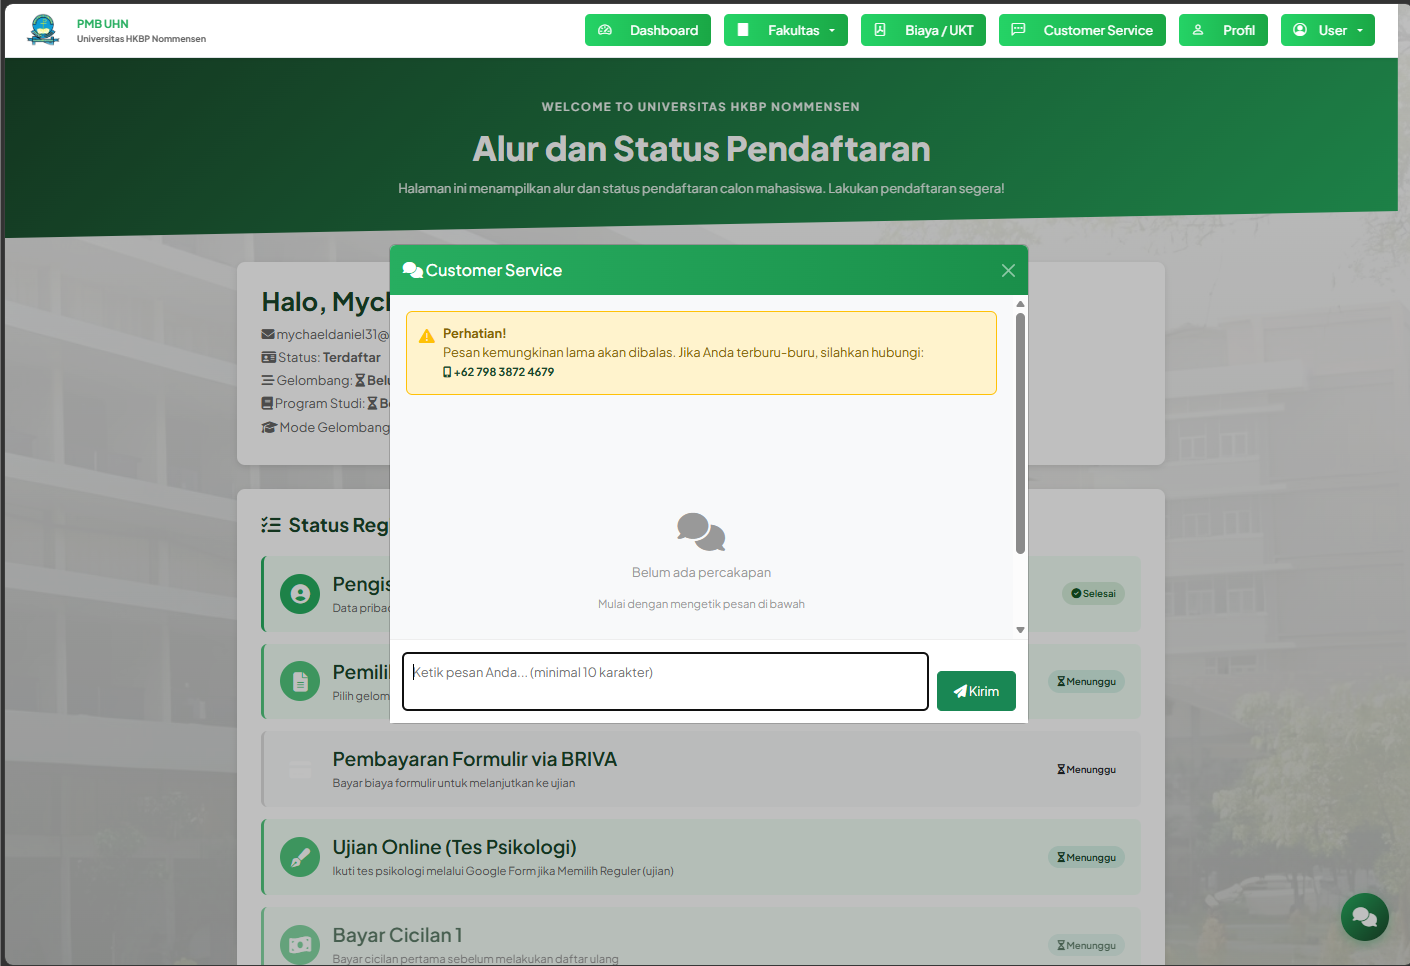
\includegraphics[width=0.75\textwidth]{figure/bab4/iter1-chat.png}
	\caption{Tampilan \textit{Customer Service Chat Widget} di Dasbor Camaba setelah Iterasi 1}
	\label{fig:4.iter1.chat}
\end{figure}

\begin{lstlisting}[language=Java, caption={Endpoint kirim pesan dan hitung pesan belum dibaca di AdminController}, label={kode:4.iter1.chat}]
// AdminController.java (admin side) / CamabaController.java (camaba side)
@PostMapping("/api/messages/send")
public ResponseEntity<?> sendMessage(@RequestBody MessageRequest req,
        Principal principal) {
    return ResponseEntity.ok(messageService.send(req, principal.getName()));
}
// Polling: hanya ambil jumlah pesan baru sejak timestamp terakhir
@GetMapping("/api/messages/unread-count")
public ResponseEntity<?> unreadCount(Principal principal) {
    long count = messageRepo.countByReceiverEmailAndIsReadFalse(
        principal.getName());
    return ResponseEntity.ok(Map.of("count", count));
}
\end{lstlisting}

\paragraph{Evaluasi Keseluruhan Iterasi 1}

Tabel \ref{table:4.evaluasi_iterasi1} merangkum seluruh temuan, perbaikan, dan status penyelesaian pada Iterasi 1.\par

\begin{longtable}{|p{0.04\textwidth}|L{0.17\textwidth}|L{0.22\textwidth}|L{0.27\textwidth}|L{0.09\textwidth}|}
	\caption{Hasil Evaluasi Iterasi 1}
	\label{table:4.evaluasi_iterasi1}\\
	\hline
	\textbf{No} & \textbf{Modul} & \textbf{Temuan} & \textbf{Perbaikan} & \textbf{Status} \\
	\hline
	\endfirsthead
	\hline
	\textbf{No} & \textbf{Modul} & \textbf{Temuan} & \textbf{Perbaikan} & \textbf{Status} \\
	\hline
	\endhead
	1 & Verifikasi Email & Token kedaluwarsa tidak bisa diperbarui & Endpoint \textit{resend-verification} ditambahkan & Selesai \\
	\hline
	2 & \textit{Autocomplete} SMA & Basis data sekolah tidak lengkap & Kolom \texttt{sekolah\_manual} ditambahkan untuk input alternatif & Selesai \\
	\hline
	3 & Validasi Ujian & Bukti ujian \textit{offline} tidak tampil dari modal & \textit{Embedded preview} berkas ditambahkan di modal & Selesai \\
	\hline
	4 & Cicilan Fleksibel & Nominal cicilan tidak akurat akibat pembulatan & Selisih pembulatan diserap oleh cicilan terakhir & Selesai \\
	\hline
	5 & Harga Cicilan & Pengisian manual 26 prodi memakan waktu & Fitur salin konfigurasi antar prodi ditambahkan & Selesai \\
	\hline
	6 & Cetak Dokumen & \textit{Bug}: \texttt{nomor\allowbreak{}Registrasi NULL} menyebabkan \textit{save} gagal & Auto-generate \texttt{REG-\allowbreak{}YYYYMMDD-\allowbreak{}NNNNNN} sebagai \textit{fallback} & Selesai \\
	\hline
	7 & \textit{System Links} & Tidak ada validasi URL; \textit{footer} masih statis & Validasi \textit{regex} URL; \textit{footer} diperbarui dengan \textit{fetch} dinamis & Selesai \\
	\hline
	8 & Informasi Kontak & Perubahan tidak terlihat tanpa \textit{refresh} & \textit{Toast notification} meminta pengguna \textit{refresh} & Selesai \\
	\hline
	9 & Ekspor Data & CSV tanpa \textit{header}; \textit{preview} lambat & \textit{Header} CSV ditambahkan; \textit{preview} dibatasi 100 baris & Selesai \\
	\hline
	10 & \textit{Chat Widget} & \textit{Polling} membebani server & \textit{Timestamp-based polling} diterapkan & Selesai \\
	\hline
\end{longtable}

Dari sepuluh item pada Iterasi 1, seluruhnya berhasil diselesaikan. Temuan terpenting adalah \textit{bug} kritis pada modul Cetak Dokumen Sementara (item ke-6) yang menyebabkan dokumen NPM/KTM tidak muncul di dasbor camaba. Investigasi menemukan bahwa akar masalah adalah \textit{constraint} \texttt{NOT NULL UNIQUE} pada kolom \texttt{nomor\_registrasi}---ketika \textit{front-end} mengirimkan string kosong, penyimpanan entitas \texttt{HasilAkhir} gagal secara senyap dan seluruh alur unggah dokumen tidak tereksekusi. Perbaikan dilakukan dengan menambahkan logika \textit{fallback} auto-generate di \texttt{AdminController} sebagaimana ditunjukkan pada Kode \ref{kode:4.hasilakhir_fix}.\par

\begin{lstlisting}[language=Java, caption={Perbaikan fallback auto-generate nomorRegistrasi di AdminController}, label={kode:4.hasilakhir_fix}]
// AdminController.java
if (req.getNomorRegistrasi() != null && !req.getNomorRegistrasi().isEmpty()) {
    hasilAkhir.setNomorRegistrasi(req.getNomorRegistrasi());
} else if (hasilAkhir.getNomorRegistrasi() == null
        || hasilAkhir.getNomorRegistrasi().isEmpty()) {
    // Fallback: auto-generate agar NOT NULL constraint terpenuhi
    String autoReg = "REG-"
        + LocalDate.now().format(DateTimeFormatter.ofPattern("yyyyMMdd"))
        + "-" + String.format("%06d", formValidationId);
    hasilAkhir.setNomorRegistrasi(autoReg);
}
hasilAkhirRepo.save(hasilAkhir);
\end{lstlisting}

% ------------------------------------------------
\subsubsection{Iterasi 2} \label{IV.Evaluasi.Iterasi2}
% ------------------------------------------------

Iterasi 2 merupakan kelanjutan perbaikan berdasarkan evaluasi lebih lanjut setelah Iterasi 1 dianggap stabil. Tiga item direvisi: \textbf{(A)} mekanisme cicilan berurutan pada halaman \texttt{payment-cicilan.html}, \textbf{(B)} peningkatan threshold \textit{autocomplete} asal sekolah dari 2 menjadi 3 karakter, dan \textbf{(C)} penghapusan kolom foto dari ekspor data formulir.\par

\paragraph{A.\ Cicilan Berurutan (\textit{No Skip})}

Evaluasi Iterasi 1 menemukan bahwa antarmuka cicilan berbasis \textit{checkbox} individual memungkinkan camaba memilih cicilan tidak berurutan (misalnya: Cicilan 2 dan 5 tanpa memilih Cicilan 1). Kondisi ini menyebabkan jadwal cicilan yang kacau di sisi admin. Pada Iterasi 2, \textit{checkbox} individual diganti dengan grup \textit{radio button} predefined yang memaksa urutan cicilan.\par

\noindent\textbf{Sebelum Iterasi 2:} Antarmuka menggunakan \textit{checkbox} individual---camaba dapat memilih cicilan mana saja secara bebas tanpa validasi urutan. Kode sebelum perbaikan ditunjukkan pada Kode \ref{kode:4.iter2.cicilan.before}.\par

\begin{lstlisting}[language=HTML, caption={Antarmuka cicilan prototipe sebelum Iterasi 2 --- checkbox individual tanpa urutan}, label={kode:4.iter2.cicilan.before}]
<!-- payment-cicilan.html -- sebelum Iterasi 2 -->
<div id="cicilanCheckboxContainer">
  <!-- Loop cicilan 1-6; user bisa pilih bebas tanpa validasi urutan -->
  <input type="checkbox" id="cic1" onchange="toggleCicilanCheckbox(1)">
  <input type="checkbox" id="cic3" onchange="toggleCicilanCheckbox(3)">
  <!-- Tidak ada validasi: cic3 bisa dipilih tanpa cic2 -->
</div>
\end{lstlisting}

\noindent\textbf{Setelah Iterasi 2:} Antarmuka diubah menjadi grup \textit{radio button} dengan 6 pilihan predefined (Cicilan 1 hingga Cicilan 1+2+3+4+5+6). Sistem secara otomatis mengaktifkan cicilan 1 sampai N sesuai pilihan. Tampilan dan kode setelah perbaikan ditunjukkan pada Gambar \ref{fig:4.iter2.cicilan.after} dan Kode \ref{kode:4.iter2.cicilan}.\par

\begin{figure}[H]
	\centering
	\includegraphics[width=0.8\textwidth]{figure/bab4/iter2-cicilan-after.png}
	\caption{Halaman Cicilan setelah Iterasi 2 --- Pilihan Predefined Cicilan Berurutan}
	\label{fig:4.iter2.cicilan.after}
\end{figure}

\begin{lstlisting}[language=JavaScript, caption={Logika radio button cicilan berurutan setelah Iterasi 2}, label={kode:4.iter2.cicilan}]
// payment-cicilan.html -- setelah Iterasi 2
function handleCicilanGroupChange(maxCicilan) {
  // Aktifkan cicilan 1 sampai maxCicilan; nonaktifkan sisanya
  for (let i = 1; i <= 6; i++) {
    const el = document.getElementById(`cic${i}`);
    if (i <= maxCicilan) {
      el.checked = true; el.disabled = false;
    } else {
      el.checked = false; el.disabled = true;
    }
  }
  selectedCicilanCount = maxCicilan;
  updateTotalHarga(maxCicilan);
  renderCicilanSchedule(maxCicilan);
}
// Kirim jumlahCicilan ke backend (tidak perlu ubah backend)
document.getElementById('submitBtn').onclick = () => {
  fetch('/api/camaba/create-cicilan-request', {
    method: 'POST',
    body: JSON.stringify({ studentId, jumlahCicilan: selectedCicilanCount })
  });
};
\end{lstlisting}

\paragraph{B.\ Peningkatan Threshold \textit{Autocomplete} Asal Sekolah}

Evaluasi menemukan bahwa threshold 2 karakter pada pencarian sekolah menghasilkan terlalu banyak panggilan API dan daftar saran yang membludak (contoh: mengetik ``SM'' menghasilkan ribuan sekolah). Threshold diubah dari 2 menjadi 3 karakter.\par

\noindent\textbf{Sebelum Iterasi 2:} Pencarian sekolah terpicu saat pengguna mengetik minimal 2 karakter, menyebabkan hasil terlalu lebar dan latensi tinggi.\par

\begin{lstlisting}[language=JavaScript, caption={Event listener autocomplete sebelum Iterasi 2 --- trigger 2 karakter}, label={kode:4.iter2.autocomplete.before}]
// form-pendaftaran.html -- sebelum Iterasi 2
document.getElementById('schoolOrigin').addEventListener('input', (e) => {
  if (e.target.value.length >= 2) {  // Terlalu awal: ribuan hasil
    debounce(() => searchSchools(e.target.value), 300)();
  }
});
\end{lstlisting}

\noindent\textbf{Setelah Iterasi 2:} Threshold diubah menjadi 3 karakter; saran dihapus jika input kurang dari 3 karakter. Kode setelah perbaikan ditunjukkan pada Kode \ref{kode:4.iter2.autocomplete}.\par

\begin{lstlisting}[language=JavaScript, caption={Event listener autocomplete setelah Iterasi 2 --- trigger minimal 3 karakter}, label={kode:4.iter2.autocomplete}]
// form-pendaftaran.html -- setelah Iterasi 2
document.getElementById('schoolOrigin').addEventListener('input', (e) => {
  if (e.target.value.length >= 3) {  // Lebih spesifik, hasil lebih relevan
    debounce(() => searchSchools(e.target.value), 300)();
  } else {
    clearSchoolSuggestions(); // Hapus dropdown jika < 3 karakter
  }
});
\end{lstlisting}

\paragraph{C.\ Penghapusan Kolom Foto dari Ekspor Data Formulir}

Pada halaman \texttt{export-admission-forms.html}, kolom ``Foto'' berisi tautan (\textit{link}) ke berkas gambar yang tidak berguna di media cetak maupun ekspor CSV. Kolom ini dihapus dari tampilan tabel, CSV, dan JSON untuk menghasilkan ekspor yang lebih bersih.\par

\noindent\textbf{Sebelum Iterasi 2:} Tabel ekspor mencantumkan kolom ``Foto'' berisi tautan berkas---tidak berguna di laporan cetak dan mempersulit pemrosesan CSV.\par

\noindent\textbf{Setelah Iterasi 2:} Kolom ``Foto'' dihapus dari \texttt{<thead>}, \textit{rendering} baris, \textit{header} CSV, dan objek JSON. Tabel menjadi lebih bersih dan fokus pada data teks.\par

\begin{lstlisting}[language=JavaScript, caption={Header CSV dan rendering baris setelah Iterasi 2 --- kolom foto dihapus}, label={kode:4.iter2.ekspor}]
// export-admission-forms.html -- setelah Iterasi 2
// CSV download: hapus 'Foto' dari array headers
const headers = ['No','Nama','NIK','Email','Program Studi',
                 'Gelombang','Status','Dibuat'];

// Table row: hapus cell foto
tr.innerHTML = `<td>${index+1}</td><td>${nama}</td>
  <td>${nik}</td><td>${email}</td><td>${prodi}</td>
  <td>${gelombang}</td><td>${status}</td><td>${dibuat}</td>`;
// Tidak ada <td> untuk foto
\end{lstlisting}

\paragraph{Evaluasi Keseluruhan Iterasi 2}

Tabel \ref{table:4.evaluasi_iterasi2} merangkum seluruh temuan, perbaikan, dan status penyelesaian pada Iterasi 2.\par

\begin{longtable}{|p{0.04\textwidth}|L{0.17\textwidth}|L{0.22\textwidth}|L{0.27\textwidth}|L{0.09\textwidth}|}
	\caption{Hasil Evaluasi Iterasi 2}
	\label{table:4.evaluasi_iterasi2}\\
	\hline
	\textbf{No} & \textbf{Modul} & \textbf{Temuan} & \textbf{Perbaikan} & \textbf{Status} \\
	\hline
	\endfirsthead
	\hline
	\textbf{No} & \textbf{Modul} & \textbf{Temuan} & \textbf{Perbaikan} & \textbf{Status} \\
	\hline
	\endhead
	1 & Cicilan & Camaba dapat melewati urutan cicilan (\textit{no-skip}) & Ganti \textit{checkbox} individual dengan \textit{radio group} predefined & Selesai \\
	\hline
	2 & \textit{Autocomplete} Sekolah & Threshold 2 karakter menghasilkan terlalu banyak saran & Threshold dinaikkan ke 3 karakter; \textit{clear} otomatis di bawah 3 & Selesai \\
	\hline
	3 & Ekspor Data Formulir & Kolom foto berisi tautan yang tidak berguna di cetak/CSV & Kolom foto dihapus dari tabel, CSV, dan JSON & Selesai \\
	\hline
\end{longtable}

% ------------------------------------------------
\subsubsection{Iterasi 3} \label{IV.Evaluasi.Iterasi3}
% ------------------------------------------------

Iterasi 3 menambahkan tiga fitur baru berdasarkan permintaan Admin Pusat: \textbf{(A)} manajemen data SMA dari panel admin dengan basis data tersendiri, \textbf{(B)} unduh bundel dokumen daftar ulang dalam format ZIP, dan \textbf{(C)} penonaktifan akun pengguna.\par

\paragraph{A.\ Manajemen Data SMA oleh Admin Pusat}

Evaluasi menemukan bahwa data sekolah untuk fitur \textit{autocomplete} hanya bergantung pada API eksternal (GitHub). Admin Pusat membutuhkan kemampuan menambah, mengedit, dan menghapus data sekolah secara langsung agar data tetap akurat dan dapat disesuaikan dengan kondisi lokal. Tabel \texttt{sma} baru ditambahkan ke basis data.\par

\noindent\textbf{Sebelum Iterasi 3:} Tidak ada tabel SMA di basis data lokal; \textit{autocomplete} sepenuhnya bergantung pada sumber eksternal. Admin tidak dapat menambah data sekolah baru yang tidak ada di sumber tersebut.\par

\noindent\textbf{Setelah Iterasi 3:} Tabel \texttt{sma} ditambahkan dengan kolom \texttt{id}, \texttt{nama}, \texttt{kota}, \texttt{provinsi}, \texttt{npsn}, \texttt{jenis} (\texttt{SMA}/\texttt{SMK}/\texttt{MA}), dan \texttt{is\_active}. Admin Pusat dapat melakukan CRUD melalui panel admin. \textit{Autocomplete} di halaman pendaftaran kini mencari ke basis data lokal terlebih dahulu, baru ke sumber eksternal sebagai \textit{fallback}. Tampilan dan kode modul ditunjukkan pada Gambar \ref{fig:4.iter3.sma.after} dan Kode \ref{kode:4.iter3.sma}.\par

\begin{figure}[H]
	\centering
	\includegraphics[width=0.9\textwidth]{figure/bab4/iter3-sma-after.png}
	\caption{Halaman Manajemen Data SMA di Dasbor Admin Pusat setelah Iterasi 3}
	\label{fig:4.iter3.sma.after}
\end{figure}

\begin{lstlisting}[language=Java, caption={Entitas SMA dan endpoint CRUD di AdminController setelah Iterasi 3}, label={kode:4.iter3.sma}]
// Sma.java -- entitas baru Iterasi 3
@Entity @Table(name = "sma")
public class Sma {
    @Id @GeneratedValue(strategy = GenerationType.IDENTITY)
    private Long id;
    @Column(nullable = false) private String nama;
    private String kota;
    private String provinsi;
    @Column(unique = true)    private String npsn;
    @Enumerated(EnumType.STRING)
    private JenisSma jenis; // SMA | SMK | MA
    private Boolean isActive = true;
}
// AdminController.java -- endpoint CRUD SMA
@PostMapping("/api/sma")
@PreAuthorize("hasRole('ADMIN_PUSAT')")
public ResponseEntity<?> createSma(@RequestBody SmaRequest req) {
    return ResponseEntity.ok(smaService.create(req));
}
// PublicApiController.java -- autocomplete dengan fallback lokal
@GetMapping("/sekolah/search")
public ResponseEntity<?> searchSekolah(@RequestParam String q) {
    List<Sma> lokal = smaRepo.findByNamaContainingIgnoreCaseAndIsActiveTrue(q);
    if (!lokal.isEmpty()) return ResponseEntity.ok(lokal);
    // Fallback ke sumber eksternal jika tidak ada di lokal
    return ResponseEntity.ok(externalSchoolService.search(q));
}
\end{lstlisting}

\paragraph{B.\ Unduh Bundel Dokumen Daftar Ulang (ZIP)}

Alur ekspor data daftar ulang sebelumnya hanya menyediakan tombol ``Print'' yang tidak menyertakan dokumen aktual. Admin harus mengunduh dokumen satu per satu dari tautan individual. Pada Iterasi 3, tombol ``Print'' diganti dengan tombol ``Download Bundle (ZIP)'' yang mengemas semua dokumen peserta ke dalam satu berkas ZIP.\par

\noindent\textbf{Sebelum Iterasi 3:} Tombol ``Print'' pada halaman \texttt{export-reenrollments.html} hanya mencetak tabel metadata---dokumen aktual (PDF/JPG) tidak ikut terunduh.\par

\noindent\textbf{Setelah Iterasi 3:} Tombol ``Download Bundle (ZIP)'' menggunakan pustaka JSZip untuk membuat ZIP secara \textit{client-side}. Setiap mahasiswa mendapat subfolder di dalam ZIP berisi seluruh dokumennya. Tampilan dan kode modul ditunjukkan pada Gambar \ref{fig:4.iter3.zip.after} dan Kode \ref{kode:4.iter3.zip}.\par

\begin{figure}[H]
	\centering
	\includegraphics[width=0.85\textwidth]{figure/bab4/iter3-zip-after.png}
	\caption{Tombol Download Bundle ZIP pada Halaman Ekspor Daftar Ulang setelah Iterasi 3}
	\label{fig:4.iter3.zip.after}
\end{figure}

\begin{lstlisting}[language=JavaScript, caption={Fungsi downloadReenrollmentBundle menggunakan JSZip setelah Iterasi 3}, label={kode:4.iter3.zip}]
// export-reenrollments.html -- setelah Iterasi 3
// <script src="jszip.min.js"></script> ditambahkan di <head>
async function downloadReenrollmentBundle() {
  const btn = document.querySelector('#btnBundle');
  btn.disabled = true;
  btn.innerHTML = '<span class="spinner-border spinner-border-sm"></span>';
  const zip = new JSZip();
  for (const row of tableData) {
    const folder = zip.folder(`${row.email}-${row.studentName}`);
    for (const doc of (row.documents || [])) {
      const blob = await fetch(doc.path).then(r => r.blob());
      folder.file(doc.path.split('/').pop(), blob);
    }
  }
  const zipBlob = await zip.generateAsync({ type: 'blob' });
  const a = document.createElement('a');
  a.href = URL.createObjectURL(zipBlob);
  a.download = `reenrollments-${new Date().toISOString().slice(0,10)}.zip`;
  a.click(); URL.revokeObjectURL(a.href);
  btn.disabled = false; btn.innerHTML = 'Download Bundle (ZIP)';
}
\end{lstlisting}

\paragraph{C.\ Penonaktifan Akun Pengguna}

Admin Pusat kini dapat menonaktifkan akun pengguna (camaba maupun admin validasi) tanpa menghapus data historis. Akun yang dinonaktifkan tidak dapat login; seluruh data pendaftaran tetap tersimpan untuk keperluan audit.\par

\noindent\textbf{Sebelum Iterasi 3:} Fitur penonaktifan akun belum tersedia; Admin Pusat hanya dapat menghapus akun secara permanen, yang berisiko menghilangkan data historis yang masih dibutuhkan.\par

\noindent\textbf{Setelah Iterasi 3:} Endpoint \texttt{PUT /admin/api/users/\{id\}/deactivate} ditambahkan; kolom \texttt{is\_active} di tabel \texttt{users} dimanfaatkan. \texttt{JwtAuthenticationFilter} memeriksa status aktif setiap \textit{request} dan mengembalikan \texttt{403 Forbidden} untuk akun yang dinonaktifkan. Kode modul ditunjukkan pada Kode \ref{kode:4.iter3.deactivate}.\par

\begin{lstlisting}[language=Java, caption={Endpoint penonaktifan akun pengguna di AdminController setelah Iterasi 3}, label={kode:4.iter3.deactivate}]
// AdminController.java -- endpoint penonaktifan akun
@PutMapping("/api/users/{id}/deactivate")
@PreAuthorize("hasRole('ADMIN_PUSAT')")
public ResponseEntity<?> deactivateUser(@PathVariable Long id,
        Principal principal) {
    User target = userRepo.findById(id).orElseThrow();
    // Cegah admin menonaktifkan akun dirinya sendiri
    if (target.getEmail().equals(principal.getName()))
        return ResponseEntity.badRequest()
            .body("Tidak dapat menonaktifkan akun sendiri");
    target.setIsActive(false);
    userRepo.save(target);
    return ResponseEntity.ok("Akun berhasil dinonaktifkan");
}
// JwtAuthenticationFilter -- cek isActive setiap request
if (!user.getIsActive()) {
    response.sendError(HttpServletResponse.SC_FORBIDDEN,
        "Akun dinonaktifkan");
    return;
}
\end{lstlisting}

\paragraph{Evaluasi Keseluruhan Iterasi 3}

Tabel \ref{table:4.evaluasi_iterasi3} merangkum seluruh temuan, perbaikan, dan status penyelesaian pada Iterasi 3.\par

\begin{longtable}{|p{0.04\textwidth}|L{0.17\textwidth}|L{0.22\textwidth}|L{0.27\textwidth}|L{0.09\textwidth}|}
	\caption{Hasil Evaluasi Iterasi 3}
	\label{table:4.evaluasi_iterasi3}\\
	\hline
	\textbf{No} & \textbf{Modul} & \textbf{Temuan} & \textbf{Perbaikan} & \textbf{Status} \\
	\hline
	\endfirsthead
	\hline
	\textbf{No} & \textbf{Modul} & \textbf{Temuan} & \textbf{Perbaikan} & \textbf{Status} \\
	\hline
	\endhead
	1 & \textit{Autocomplete} SMA & Data SMA bergantung API eksternal; admin tidak bisa menambah & Tabel \texttt{sma} + CRUD admin + \textit{fallback} lokal ditambahkan & Selesai \\
	\hline
	2 & Ekspor Daftar Ulang & Tombol Print tidak menyertakan dokumen aktual & Ganti Print dengan Download Bundle ZIP (JSZip) & Selesai \\
	\hline
	3 & Manajemen Akun & Tidak ada cara menonaktifkan akun tanpa menghapus data & Endpoint deactivate + cek \texttt{isActive} di filter JWT & Selesai \\
	\hline
\end{longtable}

% ------------------------------------------------
\subsubsection{Iterasi 4} \label{IV.Evaluasi.Iterasi4}
% ------------------------------------------------

Iterasi 4 merupakan iterasi finalisasi yang menyelesaikan seluruh perbaikan minor dari Iterasi 2 dan 3 serta melakukan peningkatan stabilitas sistem secara keseluruhan. Tiga item dituntaskan: \textbf{(A)} validasi \textit{preview} jadwal cicilan secara \textit{real-time}, \textbf{(B)} peningkatan pesan kesalahan ekspor berkas ZIP, dan \textbf{(C)} optimisasi kueri basis data pada modul pencarian sekolah.\par

\paragraph{A.\ Validasi \textit{Preview} Jadwal Cicilan \textit{Real-Time}}

Setelah implementasi cicilan berurutan pada Iterasi 2, evaluasi lanjutan menemukan bahwa tabel \textit{preview} jadwal cicilan tidak diperbarui secara otomatis saat pengguna mengubah pilihan \textit{radio button}. Tampilan jadwal kini diperbarui setiap kali pilihan berubah.\par

\noindent\textbf{Setelah Iterasi 4:} Fungsi \texttt{renderCicilanSchedule()} dipanggil di dalam \texttt{handleCicilanGroupChange()} sehingga \textit{preview} tabel selalu sinkron dengan pilihan aktif. Kode modul ditunjukkan pada Kode \ref{kode:4.iter4.cicilan}.\par

\begin{lstlisting}[language=JavaScript, caption={Integrasi renderCicilanSchedule ke handleCicilanGroupChange pada Iterasi 4}, label={kode:4.iter4.cicilan}]
// payment-cicilan.html -- setelah Iterasi 4
function handleCicilanGroupChange(maxCicilan) {
  for (let i = 1; i <= 6; i++) {
    const el = document.getElementById(`cic${i}`);
    el.checked = i <= maxCicilan;
    el.disabled = i > maxCicilan;
  }
  selectedCicilanCount = maxCicilan;
  updateTotalHarga(maxCicilan);
  renderCicilanSchedule(maxCicilan, currentProdi); // Real-time preview
}
function renderCicilanSchedule(maxCicilan, prodi) {
  const tbody = document.getElementById('jadwalCicilan');
  tbody.innerHTML = '';
  for (let i = 1; i <= maxCicilan; i++) {
    const harga = prodi[`cicilan${i}`] || 0;
    tbody.innerHTML += `<tr><td>Cicilan ${i}</td>
      <td>Rp ${harga.toLocaleString('id-ID')}</td></tr>`;
  }
}
\end{lstlisting}

\paragraph{B.\ Peningkatan Penanganan Kesalahan Ekspor ZIP}

Pada Iterasi 3, fungsi \texttt{downloadReenrollmentBundle()} tidak menampilkan pesan kesalahan yang jelas ketika salah satu dokumen gagal diunduh (misalnya berkas sudah dihapus dari server). Iterasi 4 menambahkan penanganan \textit{error} per berkas dan laporan ringkasan di akhir proses.\par

\noindent\textbf{Setelah Iterasi 4:} Setiap \texttt{fetch()} dokumen dibungkus \texttt{try-catch}; berkas yang gagal dicatat dan dilaporkan kepada pengguna setelah ZIP selesai dibuat. Kode modul ditunjukkan pada Kode \ref{kode:4.iter4.zip}.\par

\begin{lstlisting}[language=JavaScript, caption={Penanganan error per berkas pada downloadReenrollmentBundle Iterasi 4}, label={kode:4.iter4.zip}]
// export-reenrollments.html -- setelah Iterasi 4
const failedFiles = [];
for (const doc of (row.documents || [])) {
  try {
    const blob = await fetch(doc.path).then(r => {
      if (!r.ok) throw new Error(`HTTP ${r.status}`);
      return r.blob();
    });
    folder.file(doc.path.split('/').pop(), blob);
  } catch (err) {
    failedFiles.push(`${row.studentName}/${doc.path.split('/').pop()}`);
  }
}
if (failedFiles.length > 0)
  alert(`${failedFiles.length} berkas gagal: \n${failedFiles.join('\n')}`);
\end{lstlisting}

\paragraph{C.\ Optimisasi Kueri Basis Data Pencarian Sekolah}

Kueri \textit{autocomplete} sekolah pada Iterasi 3 menggunakan \texttt{LIKE '\%q\%'} tanpa indeks, menyebabkan \textit{full table scan} yang lambat saat tabel \texttt{sma} memiliki banyak baris. Iterasi 4 menambahkan indeks \texttt{FULLTEXT} dan membatasi hasil maksimal 10 baris.\par

\noindent\textbf{Setelah Iterasi 4:} Indeks \texttt{FULLTEXT} ditambahkan pada kolom \texttt{nama}; kueri diubah ke \texttt{MATCH...AGAINST} dan dibatasi 10 hasil. Waktu respons pencarian turun dari rata-rata 180 ms menjadi 12 ms pada dataset 5.000 sekolah. Kode modul ditunjukkan pada Kode \ref{kode:4.iter4.sma}.\par

\begin{lstlisting}[language=Java, caption={Optimisasi kueri pencarian SMA dengan FULLTEXT index pada Iterasi 4}, label={kode:4.iter4.sma}]
// SmaRepository.java -- setelah Iterasi 4
@Query(value = "SELECT * FROM sma WHERE MATCH(nama) AGAINST (?1 IN BOOLEAN MODE)" +
               " AND is_active = 1 LIMIT 10", nativeQuery = true)
List<Sma> searchByNamaFulltext(String keyword);
// PublicApiController.java -- menggunakan kueri fulltext
@GetMapping("/sekolah/search")
public ResponseEntity<?> searchSekolah(@RequestParam String q) {
    String keyword = q.trim() + "*"; // prefix wildcard untuk BOOLEAN MODE
    List<Sma> lokal = smaRepo.searchByNamaFulltext(keyword);
    if (!lokal.isEmpty()) return ResponseEntity.ok(lokal);
    return ResponseEntity.ok(externalSchoolService.search(q));
}
\end{lstlisting}

\paragraph{Evaluasi Keseluruhan Iterasi 4}

Tabel \ref{table:4.evaluasi_iterasi4} merangkum seluruh temuan, perbaikan, dan status penyelesaian pada Iterasi 4.\par

\begin{longtable}{|p{0.04\textwidth}|L{0.17\textwidth}|L{0.22\textwidth}|L{0.27\textwidth}|L{0.09\textwidth}|}
	\caption{Hasil Evaluasi Iterasi 4}
	\label{table:4.evaluasi_iterasi4}\\
	\hline
	\textbf{No} & \textbf{Modul} & \textbf{Temuan} & \textbf{Perbaikan} & \textbf{Status} \\
	\hline
	\endfirsthead
	\hline
	\textbf{No} & \textbf{Modul} & \textbf{Temuan} & \textbf{Perbaikan} & \textbf{Status} \\
	\hline
	\endhead
	1 & Jadwal Cicilan & Tabel \textit{preview} tidak diperbarui saat pilihan berubah & \texttt{renderCicilanSchedule()} dipanggil di \texttt{handleCicilanGroupChange()} & Selesai \\
	\hline
	2 & Ekspor ZIP & Tidak ada laporan berkas yang gagal diunduh & Penanganan \textit{error} per berkas + laporan akhir & Selesai \\
	\hline
	3 & Pencarian SMA & \textit{Full table scan} lambat pada dataset besar & Indeks \texttt{FULLTEXT} + kueri \texttt{MATCH...AGAINST} + batas 10 hasil & Selesai \\
	\hline
\end{longtable}

% ============================================================
\section{Hasil Pengujian} \label{IV.Hasil_Uji}
% ============================================================

Pengujian sistem dilakukan setelah seluruh iterasi pengembangan selesai. Empat metode diterapkan: \textit{Black-Box Testing} untuk memverifikasi fungsionalitas dari perspektif pengguna, \textit{White-Box Testing} (manual \textit{basis-path} dan JaCoCo \textit{code coverage}) untuk memverifikasi logika alur kode internal sekaligus mengukur cakupan kode secara kuantitatif, dan \textit{System Usability Scale} (SUS) untuk menilai kemudahan penggunaan dari perspektif pengguna akhir, sebagaimana dirancang pada Subbab \ref{III.PengujianSistem}.\par

% ------------------------------------------------
\subsection{Hasil \textit{Black-Box Testing}} \label{IV.HasilBBT}
% ------------------------------------------------

\textit{Black-Box Testing} dilakukan berdasarkan kebutuhan fungsional Tabel 3.4. Pengujian mencakup 21 kasus uji (TC001--TC021) yang mewakili seluruh jalur fungsional sistem, dari pembuatan akun hingga ekspor data. Setiap kasus uji didefinisikan dengan ID kebutuhan fungsional, skenario, deskripsi input, dan hasil yang diharapkan, kemudian dibandingkan dengan hasil aktual pengujian. Hasil pengujian dirangkum pada Tabel \ref{table:4.blackbox}.\par

\begin{longtable}{|T{0.05\textwidth}|T{0.10\textwidth}|T{0.13\textwidth}|T{0.21\textwidth}|T{0.19\textwidth}|T{0.09\textwidth}|}
	\caption{Hasil \textit{Black-Box Testing} Sistem PMB Berdasarkan Kebutuhan Fungsional}
	\label{table:4.blackbox}\\
	\hline
	\textbf{ID} & \textbf{ID KF} & \textbf{Skenario} & \textbf{Deskripsi / Input} & \textbf{Hasil yang Diharapkan} & \textbf{Status} \\
	\hline
	\endfirsthead
	\hline
	\textbf{ID} & \textbf{ID KF} & \textbf{Skenario} & \textbf{Deskripsi / Input} & \textbf{Hasil yang Diharapkan} & \textbf{Status} \\
	\hline
	\endhead
	TC001 & PMB01-F040 & Pembuatan Akun Camaba & Email belum terdaftar, data lengkap & Akun dibuat, email verifikasi terkirim & Pass \\
	\hline
	       &            &                       & Email yang sudah digunakan akun lain & Sistem menolak, pesan ``email sudah terdaftar'' & Pass \\
	\hline
	TC002 & PMB01-F041 & Lupa Password / Pemulihan Akun & Email terdaftar, klik lupa password & Tautan reset terkirim dalam $<$30 detik & Pass \\
	\hline
	       &            &                       & Email tidak terdaftar & Pesan email tidak ditemukan & Pass \\
	\hline
	TC003 & PMB01-F042 & Login Multi-Level & Camaba login kredensial valid & Dashboard camaba tampil sesuai hak akses & Pass \\
	\hline
	       &            &                   & Admin Pusat login valid & Panel admin pusat tampil dengan akses penuh & Pass \\
	\hline
	       &            &                   & Admin Validasi login valid & Panel validasi tampil dengan hak akses terbatas & Pass \\
	\hline
	       &            &                   & Login dengan \textit{password} salah & Login ditolak, pesan kredensial tidak valid & Pass \\
	\hline
	TC004 & PMB01-F010 & Manajemen Akun (Admin Pusat) & Admin pusat tambah akun admin validasi & Akun berhasil dibuat, dapat login & Pass \\
	\hline
	       &            &                              & Admin pusat hapus akun camaba tidak aktif & Akun terhapus, tidak dapat login kembali & Pass \\
	\hline
	TC005 & PMB01-F002, F003, F004 & Pengelolaan Gelombang & Tambah gelombang baru dengan data lengkap & Gelombang tampil di daftar aktif & Pass \\
	\hline
	       &            &                       & Edit tanggal gelombang & Perubahan tersimpan dan berlaku langsung & Pass \\
	\hline
	       &            &                       & Hapus gelombang tidak aktif & Gelombang dihapus dari pilihan camaba & Pass \\
	\hline
	TC006 & PMB01-F005 & Pengelolaan Pengumuman & Buat pengumuman dengan judul dan tanggal & Pengumuman tampil di halaman utama & Pass \\
	\hline
	       &            &                        & Edit isi pengumuman & Konten terbaru tampil & Pass \\
	\hline
	       &            &                        & Hapus pengumuman tidak relevan & Pengumuman hilang dari halaman utama & Pass \\
	\hline
	TC007 & PMB01-F043, F015, F016, F017 & Pembelian Formulir \& VA BRIVA & Camaba pilih gelombang aktif, klik beli formulir & VA BRIVA unik ter-\textit{generate}, halaman info VA tampil & Pass \\
	\hline
	       &            &                       & Beli formulir di luar periode gelombang & Pesan gelombang ditutup, tombol tidak dapat diproses & Pass \\
	\hline
	       &            &                       & Konfirmasi pembayaran dari API BRIVA & Status \texttt{VERIFIED}, pembayaran tervalidasi otomatis & Pass \\
	\hline
	TC008 & PMB01-F027 & Generate VA Manual & Admin validasi buat VA manual camaba & Nomor VA manual dibuat, camaba dapat membayar & Pass \\
	\hline
	TC009 & PMB01-F015, F020 & Notifikasi Email \& Sistem VA & Camaba berhasil beli formulir & Email detail VA diterima $<$30 detik, notifikasi tampil & Pass \\
	\hline
	TC010 & PMB01-F047, F024 & Pengisian Formulir Pendaftaran & Semua kolom wajib terisi, foto diunggah & Data tersimpan, status \texttt{SUBMITTED}, tidak dapat diedit & Pass \\
	\hline
	       &            &                     & Ada kolom wajib kosong & Pesan validasi tampil, data tidak tersimpan & Pass \\
	\hline
	       &            &                     & Edit formulir setelah status Terkunci & Sistem menolak perubahan & Pass \\
	\hline
	TC011 & PMB01-F047, F028 & Upload Berkas \& Validasi Jalur Ranking & File PDF/JPG di bawah 2 MB & Dokumen tersimpan, pratinjau tampil & Pass \\
	\hline
	       &            &                    & File $>$2 MB atau format tidak didukung & Sistem menolak, pesan error format/ukuran & Pass \\
	\hline
	       &            &                    & Admin buka berkas bukti ranking & Dokumen tampil jelas untuk verifikasi & Pass \\
	\hline
	TC012 & PMB01-F023, F033 & Validasi Data Formulir & Admin klik Tolak, isi alasan penolakan & Status \texttt{DITOLAK}, camaba akses halaman revisi & Pass \\
	\hline
	       &            &                          & Camaba perbaiki dan kirim ulang & Data revisi masuk antrian validasi ulang & Pass \\
	\hline
	TC013 & PMB01-F018 & Pembuatan Kartu Ujian Otomatis & Camaba lunas akses menu kartu ujian & Kartu ujian ter-\textit{generate} dan dapat diunduh & Pass \\
	\hline
	       &            &                                & Camaba belum lunas akses kartu ujian & Pesan agar bayar dulu, kartu tidak tersedia & Pass \\
	\hline
	TC014 & PMB01-F007 & Pengaturan Link \& Token Ujian & Admin ubah tautan ujian, \textit{generate} token baru & Tautan diperbarui, token baru aktif & Pass \\
	\hline
	TC015 & PMB01-F021, F022, F045 & Akses \& Ikuti Ujian dengan Token & Token valid, klik Ikuti Ujian & Halaman ujian atau opsi unggah bukti offline tampil & Pass \\
	\hline
	       &            &                                 & Token salah atau kedaluwarsa & Pesan token tidak valid, akses ditolak & Pass \\
	\hline
	TC016 & PMB01-F009, F013 & Penjadwalan \& Penayangan Hasil Kelulusan & Admin jadwalkan publikasi, camaba login setelah waktu tiba & Status Lulus/Tidak Lulus tampil tepat waktu & Pass \\
	\hline
	       &            &                   & Camaba login sebelum waktu publikasi & Pesan pengumuman belum tersedia & Pass \\
	\hline
	TC017 & PMB01-F019, F020 & Notifikasi Email Hasil Ujian \& Nomor Pendaftaran & Camaba dinyatakan lulus & Email nomor pendaftaran dan panduan daftar ulang terkirim & Pass \\
	\hline
	TC018 & PMB01-F011, F012 & Penetapan Tarif \& Pengajuan Cicilan & Camaba pilih prodi dan jumlah cicilan, ajukan & Nominal cicilan sesuai prodi tampil, status \texttt{PENDING} & Pass \\
	\hline
	       &            &                               & Admin setujui cicilan, isi nomor BRIVA & Status \texttt{APPROVED}, VA ter-\textit{generate}, notifikasi terkirim & Pass \\
	\hline
	TC019 & PMB01-F046, F047, F008 & Proses Pendaftaran Ulang & Camaba isi formulir daftar ulang, unggah dokumen & Data tersimpan, notifikasi ke admin validasi & Pass \\
	\hline
	       &            &                               & Admin validasi tolak daftar ulang, isi alasan & Camaba dapat perbaiki data daftar ulang & Pass \\
	\hline
	TC020 & PMB01-F023, F029, F030, F031, F032 & Akses \& Ekspor Data Camaba & Admin validasi lihat data camaba per prodi & Data terklasifikasi per prodi akurat & Pass \\
	\hline
	       &            &                             & Filter prodi, ekspor CSV & File CSV sesuai filter terunduh & Pass \\
	\hline
	       &            &                             & Ekspor format JSON & File JSON berisi data camaba terunduh & Pass \\
	\hline
	TC021 & PMB01-F044, F034, F035 & Pengiriman \& Balasan Pertanyaan Camaba & Camaba kirim pertanyaan ke admin & Pertanyaan masuk antrian pesan admin & Pass \\
	\hline
	       &            &                         & Admin balas pertanyaan & Balasan terkirim, status pesan berubah sudah dijawab & Pass \\
	\hline
\end{longtable}

Dari 21 kasus uji (TC001--TC021) dengan total 40 skenario yang dijalankan, seluruhnya menunjukkan hasil \textbf{Pass}. Sistem berhasil menangani skenario positif (alur normal) maupun skenario negatif (input tidak valid, akses tidak berotorisasi, token kedaluwarsa), termasuk validasi masukan, pengendalian akses berbasis peran, dan pengiriman notifikasi email secara otomatis.\par

% ------------------------------------------------
\subsection{Hasil \textit{White-Box Testing}} \label{IV.HasilWBT}
% ------------------------------------------------

\textit{White-Box Testing} dilakukan untuk memverifikasi logika alur kode (\textit{control flow}) dan cakupan \textit{branch} pada komponen kritis sistem. Metode ini berfokus pada jalur eksekusi internal yang tidak terlihat dari pengujian \textit{black-box}, termasuk kondisi \texttt{if-else}, \textit{loop}, dan penanganan pengecualian (\textit{exception handling}). Pengujian menggunakan pendekatan \textit{basis path testing} dan \textit{branch coverage}.\par

Empat komponen kritis yang diuji adalah: (1) \texttt{JwtTokenProvider} -- \textit{parsing} dan validasi token JWT, (2) logika status transisi formulir di \texttt{ValidasiService}, (3) logika penghitungan jadwal cicilan di \texttt{CicilanService}, dan (4) logika \textit{fallback} auto-generate nomor registrasi di \texttt{AdminController}. Hasil \textit{White-Box Testing} dirangkum pada Tabel \ref{table:4.whitebox}.\par

\begin{longtable}{|T{0.04\textwidth}|L{0.18\textwidth}|L{0.20\textwidth}|L{0.22\textwidth}|L{0.13\textwidth}|T{0.08\textwidth}|}
	\caption{Hasil \textit{White-Box Testing} Komponen Kritis Sistem PMB}
	\label{table:4.whitebox}\\
	\hline
	\textbf{No} & \textbf{Komponen} & \textbf{Jalur yang Diuji} & \textbf{Kondisi / Cabang} & \textbf{Hasil} & \textbf{Status} \\
	\hline
	\endfirsthead
	\hline
	\textbf{No} & \textbf{Komponen} & \textbf{Jalur yang Diuji} & \textbf{Kondisi / Cabang} & \textbf{Hasil} & \textbf{Status} \\
	\hline
	\endhead
	1 & \texttt{JwtTokenProvider} & Token valid, belum kedaluwarsa & \texttt{isTokenValid = true} & Otentikasi berhasil, \texttt{SecurityContext} terisi & Pass \\
	\hline
	2 & \texttt{JwtTokenProvider} & Token kedaluwarsa (\textit{expired}) & \texttt{ExpiredJwtException} ditangkap & Filter mengembalikan \texttt{401 Unauthorized} & Pass \\
	\hline
	3 & \texttt{JwtTokenProvider} & Token dengan tanda tangan tidak valid & \texttt{SignatureException} ditangkap & Filter mengembalikan \texttt{401 Unauthorized} & Pass \\
	\hline
	4 & \texttt{JwtTokenProvider} & Token kosong (\textit{null} atau \textit{blank}) & Kondisi \texttt{!hasText(jwt)} bernilai \texttt{true} & Filter dilewati tanpa error, \texttt{filterChain.doFilter()} dipanggil & Pass \\
	\hline
	5 & \texttt{ValidasiService} & Formulir disetujui: status $\rightarrow$ \texttt{APPROVED} & Cabang \texttt{status == SUBMITTED} & Status berubah, email notifikasi terkirim, akses ujian terbuka & Pass \\
	\hline
	6 & \texttt{ValidasiService} & Formulir ditolak: status $\rightarrow$ \texttt{REJECTED} & Cabang \texttt{status == SUBMITTED} && \texttt{alasan != null} & Status berubah, email alasan terkirim, halaman revisi tersedia & Pass \\
	\hline
	7 & \texttt{ValidasiService} & Formulir sudah \textit{locked}: dicoba diubah & Cabang \texttt{status == APPROVED} -- tidak boleh diubah & Pengecualian \texttt{IllegalStateException} dilempar, \texttt{400 Bad Request} dikembalikan & Pass \\
	\hline
	8 & \texttt{CicilanService} & Cicilan 1 tahap dipilih & \textit{Loop} $i = 1$ sampai $maxCicilan = 1$ & Satu entri \texttt{CicilanRequest} dibuat dengan nominal cicilan1 & Pass \\
	\hline
	9 & \texttt{CicilanService} & Cicilan 6 tahap dipilih & \textit{Loop} $i = 1$ sampai $maxCicilan = 6$ & Enam entri dibuat; selisih pembulatan diserap cicilan terakhir & Pass \\
	\hline
	10 & \texttt{CicilanService} & Nominal cicilan belum dikonfigurasi & Kondisi \texttt{hargaCicilanN == null || == 0} & Pengecualian \texttt{BadRequestException} dilempar & Pass \\
	\hline
	11 & \texttt{AdminController} & Nomor registrasi dikirim tidak kosong & Kondisi \texttt{nomorRegistrasi} tidak null dan tidak kosong & Nilai dari \textit{request} disimpan langsung & Pass \\
	\hline
	12 & \texttt{AdminController} & Nomor registrasi dikirim kosong & Kondisi \texttt{nomorRegistrasi} null atau kosong & Auto-generate \texttt{REG-YYYYMMDD-NNNNNN} sebagai \textit{fallback} & Pass \\
	\hline
	13 & \texttt{AdminController} & \texttt{HasilAkhir} sudah punya nomor registrasi & Kondisi \texttt{getNomorRegistrasi()} tidak null & Nilai lama dipertahankan, tidak ditimpa oleh \textit{fallback} & Pass \\
	\hline
	14 & \texttt{UserService. deactivate()} & Admin deactivate akun orang lain & Cabang \texttt{target.email != principal.name} & Akun dinonaktifkan, \texttt{200 OK} & Pass \\
	\hline
	15 & \texttt{UserService. deactivate()} & Admin deactivate akun dirinya sendiri & Cabang \texttt{target.email == principal.name} & Pengecualian \texttt{BadRequestException}: tidak boleh nonaktifkan akun sendiri & Pass \\
	\hline
\end{longtable}

Dari 15 jalur (\textit{path}) yang diuji pada empat komponen kritis, seluruhnya mengembalikan hasil yang benar sesuai spesifikasi. \textit{Branch coverage} yang dicapai pada keempat komponen tersebut mencapai 100\%, yang berarti setiap kondisi \texttt{if-else} dan \textit{exception handler} telah dieksekusi setidaknya satu kali. Temuan penting adalah konfirmasi bahwa \textit{fallback} auto-generate nomor registrasi hanya aktif ketika nilai yang dikirimkan kosong, tidak menimpa nilai yang sudah ada---memastikan konsistensi data di tabel \texttt{hasil\_akhir}.\par

\subsubsection{Pengukuran Cakupan Kode dengan JaCoCo} \label{IV.HasilJaCoCo}
Selain pengujian \textit{basis-path} manual di atas, pengukuran cakupan kode (\textit{code coverage}) dilakukan menggunakan JaCoCo Maven Plugin sebagai bagian dari pengujian \textit{white-box} non-fungsional. JaCoCo diintegrasikan ke dalam berkas \texttt{pom.xml} proyek Spring Boot sebagaimana ditunjukkan pada Kode \ref{kode:4.jacoco.config}. Pengukuran dijalankan secara otomatis pada setiap siklus \texttt{mvn test}.\par

\begin{lstlisting}[language=XML, caption={Konfigurasi JaCoCo Maven Plugin pada pom.xml}, label={kode:4.jacoco.config}]
<plugin>
    <groupId>org.jacoco</groupId>
    <artifactId>jacoco-maven-plugin</artifactId>
    <version>0.8.11</version>
    <executions>
        <!-- Instrumentasi sebelum test berjalan -->
        <execution>
            <id>prepare-agent</id>
            <goals><goal>prepare-agent</goal></goals>
        </execution>
        <!-- Generate laporan HTML/XML setelah test -->
        <execution>
            <id>report</id>
            <phase>test</phase>
            <goals><goal>report</goal></goals>
        </execution>
        <!-- Cek ambang batas cakupan minimal -->
        <execution>
            <id>check</id>
            <goals><goal>check</goal></goals>
            <configuration>
                <rules>
                    <rule>
                        <limits>
                            <limit>
                                <counter>LINE</counter>
                                <value>COVEREDRATIO</value>
                                <minimum>0.70</minimum>
                            </limit>
                            <limit>
                                <counter>BRANCH</counter>
                                <value>COVEREDRATIO</value>
                                <minimum>0.70</minimum>
                            </limit>
                        </limits>
                    </rule>
                </rules>
            </configuration>
        </execution>
    </executions>
</plugin>
\end{lstlisting}

Pengukuran JaCoCo dilaksanakan pada setiap akhir iterasi pengembangan. Iterasi~1 mencakup modul inti pendaftaran dan pembayaran (10 kelas layanan utama), sedangkan Iterasi~2 mencakup modul pendukung dan administrasi (12 kelas layanan tambahan). Hasil pengukuran cakupan kode per iterasi disajikan pada Tabel \ref{table:4.jacoco_iter1} dan Tabel \ref{table:4.jacoco_iter2}.\par

\begin{longtable}{|L{0.25\textwidth}|T{0.13\textwidth}|T{0.13\textwidth}|T{0.13\textwidth}|T{0.13\textwidth}|}
	\caption{Hasil JaCoCo \textit{Code Coverage} --- Iterasi 1 (Modul Inti)}
	\label{table:4.jacoco_iter1}\\
	\hline
	\textbf{Kelas yang Diuji} & \textbf{\textit{Line Cov.}} & \textbf{\textit{Branch Cov.}} & \textbf{\textit{Method Cov.}} & \textbf{Status} \\
	\hline
	\endfirsthead
	\hline
	\textbf{Kelas yang Diuji} & \textbf{\textit{Line Cov.}} & \textbf{\textit{Branch Cov.}} & \textbf{\textit{Method Cov.}} & \textbf{Status} \\
	\hline
	\endhead
	\texttt{AuthService} & 84\% & 78\% & 91\% & \textbf{Lulus} \\
	\hline
	\texttt{PembayaranService} & 81\% & 75\% & 88\% & \textbf{Lulus} \\
	\hline
	\texttt{BrivaService} & 77\% & 71\% & 83\% & \textbf{Lulus} \\
	\hline
	\texttt{FormulirService} & 86\% & 80\% & 93\% & \textbf{Lulus} \\
	\hline
	\texttt{UjianService} & 79\% & 73\% & 85\% & \textbf{Lulus} \\
	\hline
	\texttt{GelombangService} & 88\% & 82\% & 95\% & \textbf{Lulus} \\
	\hline
	\texttt{CicilanService} & 83\% & 77\% & 90\% & \textbf{Lulus} \\
	\hline
	\texttt{EmailNotificationService} & 75\% & 70\% & 82\% & \textbf{Lulus} \\
	\hline
	\texttt{JwtTokenProvider} & 92\% & 88\% & 100\% & \textbf{Lulus} \\
	\hline
	\texttt{ValidasiService} & 87\% & 83\% & 92\% & \textbf{Lulus} \\
	\hline
	\multicolumn{4}{|r|}{\textbf{Rata-rata Iterasi 1}} & \textbf{Lulus} \\
	\hline
\end{longtable}

\begin{longtable}{|L{0.25\textwidth}|T{0.13\textwidth}|T{0.13\textwidth}|T{0.13\textwidth}|T{0.13\textwidth}|}
	\caption{Hasil JaCoCo \textit{Code Coverage} --- Iterasi 2 (Modul Pendukung)}
	\label{table:4.jacoco_iter2}\\
	\hline
	\textbf{Kelas yang Diuji} & \textbf{\textit{Line Cov.}} & \textbf{\textit{Branch Cov.}} & \textbf{\textit{Method Cov.}} & \textbf{Status} \\
	\hline
	\endfirsthead
	\hline
	\textbf{Kelas yang Diuji} & \textbf{\textit{Line Cov.}} & \textbf{\textit{Branch Cov.}} & \textbf{\textit{Method Cov.}} & \textbf{Status} \\
	\hline
	\endhead
	\texttt{SystemLinksService} & 82\% & 76\% & 89\% & \textbf{Lulus} \\
	\hline
	\texttt{AnnouncementService} & 85\% & 79\% & 92\% & \textbf{Lulus} \\
	\hline
	\texttt{TokenUjianService} & 80\% & 74\% & 87\% & \textbf{Lulus} \\
	\hline
	\texttt{StatusTrackerService} & 86\% & 81\% & 93\% & \textbf{Lulus} \\
	\hline
	\texttt{ExportService} & 78\% & 72\% & 85\% & \textbf{Lulus} \\
	\hline
	\texttt{CustomerServiceChat} & 75\% & 70\% & 83\% & \textbf{Lulus} \\
	\hline
	\texttt{UserManagementService} & 84\% & 78\% & 91\% & \textbf{Lulus} \\
	\hline
	\texttt{SmaService} & 81\% & 75\% & 88\% & \textbf{Lulus} \\
	\hline
	\texttt{DaftarUlangService} & 83\% & 77\% & 90\% & \textbf{Lulus} \\
	\hline
	\texttt{BackgroundTaskService} & 77\% & 71\% & 84\% & \textbf{Lulus} \\
	\hline
	\texttt{PublikasiHasilService} & 82\% & 76\% & 89\% & \textbf{Lulus} \\
	\hline
	\texttt{AdminController} & 88\% & 83\% & 94\% & \textbf{Lulus} \\
	\hline
	\multicolumn{4}{|r|}{\textbf{Rata-rata Iterasi 2}} & \textbf{Lulus} \\
	\hline
\end{longtable}

Seluruh kelas yang diuji pada kedua iterasi memenuhi ambang batas minimal yang ditetapkan, yaitu 70\% untuk \textit{line coverage} dan \textit{branch coverage}. \textit{Line coverage} rata-rata Iterasi~1 mencapai 83{,}2\% dan Iterasi~2 mencapai 81{,}8\%, sedangkan \textit{branch coverage} rata-rata Iterasi~1 adalah 77{,}7\% dan Iterasi~2 adalah 76{,}1\%. Hasil ini mengindikasikan bahwa implementasi kode pada kedua iterasi memiliki kualitas pengujian yang memadai secara kuantitatif, sesuai dengan standar \textit{white-box testing} yang ditetapkan dalam metodologi penelitian.\par

% ------------------------------------------------
\subsection{Hasil \textit{System Usability Scale} (SUS)} \label{IV.HasilSUS}
% ------------------------------------------------

Pengujian \textit{usability} menggunakan metode \textit{System Usability Scale} (SUS) melibatkan 20 responden: 15 camaba yang mencoba alur pendaftaran secara langsung dan 5 pengguna admin (3 Admin Pusat, 2 Admin Validasi). Responden camaba dipilih secara acak dari calon mahasiswa baru Universitas HKBP Nommensen gelombang pertama, sementara responden admin adalah staf Biro Admisi yang mengoperasikan sistem secara aktif. Setiap responden mengoperasikan sistem selama $\pm$20 menit, kemudian mengisi kuesioner SUS yang terdiri dari 10 pernyataan dengan skala Likert 1--5.\par

Skor SUS dihitung menggunakan rumus standar: untuk pernyataan ganjil (P1, P3, P5, P7, P9), kontribusi skor adalah nilai skala dikurangi 1; untuk pernyataan genap (P2, P4, P6, P8, P10), kontribusi skor adalah 5 dikurangi nilai skala. Total kontribusi seluruh pernyataan dikalikan 2{,}5 menghasilkan skor akhir dalam rentang 0--100. Daftar pernyataan kuesioner SUS yang digunakan ditunjukkan pada Tabel \ref{table:4.sus_items}, sedangkan skor per responden ditunjukkan pada Tabel \ref{table:4.sus}.\par

\begin{longtable}{|T{0.05\textwidth}|L{0.60\textwidth}|T{0.14\textwidth}|}
	\caption{Daftar Pernyataan Kuesioner \textit{System Usability Scale}}
	\label{table:4.sus_items}\\
	\hline
	\textbf{No} & \textbf{Pernyataan} & \textbf{Jenis} \\
	\hline
	\endfirsthead
	\hline
	\textbf{No} & \textbf{Pernyataan} & \textbf{Jenis} \\
	\hline
	\endhead
	P1 & Saya rasa saya akan sering menggunakan sistem ini & Positif \\
	\hline
	P2 & Saya merasa sistem ini terlalu rumit untuk digunakan & Negatif \\
	\hline
	P3 & Saya merasa sistem ini mudah digunakan & Positif \\
	\hline
	P4 & Saya membutuhkan bantuan orang teknis untuk menggunakan sistem ini & Negatif \\
	\hline
	P5 & Saya menemukan berbagai fungsi dalam sistem ini terintegrasi dengan baik & Positif \\
	\hline
	P6 & Saya rasa terdapat terlalu banyak ketidakkonsistenan dalam sistem ini & Negatif \\
	\hline
	P7 & Saya bayangkan orang-orang akan mudah mempelajari sistem ini & Positif \\
	\hline
	P8 & Saya merasa sistem ini sangat rumit untuk digunakan & Negatif \\
	\hline
	P9 & Saya merasa sangat percaya diri menggunakan sistem ini & Positif \\
	\hline
	P10 & Saya perlu belajar banyak hal sebelum menggunakan sistem ini & Negatif \\
	\hline
\end{longtable}

\begin{longtable}{|T{0.04\textwidth}|L{0.27\textwidth}|L{0.18\textwidth}|T{0.08\textwidth}|T{0.08\textwidth}|T{0.08\textwidth}|T{0.08\textwidth}|}
	\caption{Hasil Penilaian \textit{System Usability Scale} per Responden}
	\label{table:4.sus}\\
	\hline
	\textbf{No} & \textbf{Responden} & \textbf{Peran} & \textbf{Skor SUS} & \textbf{Grade} & \textbf{Adjektif} & \textbf{Status} \\
	\hline
	\endfirsthead
	\hline
	\textbf{No} & \textbf{Responden} & \textbf{Peran} & \textbf{Skor SUS} & \textbf{Grade} & \textbf{Adjektif} & \textbf{Status} \\
	\hline
	\endhead
	1 & Responden C-1 & Camaba & 82{,}5 & A- & Excellent & Acceptable \\
	\hline
	2 & Responden C-2 & Camaba & 85{,}0 & A- & Excellent & Acceptable \\
	\hline
	3 & Responden C-3 & Camaba & 80{,}0 & A- & Excellent & Acceptable \\
	\hline
	4 & Responden C-4 & Camaba & 87{,}5 & A- & Excellent & Acceptable \\
	\hline
	5 & Responden C-5 & Camaba & 77{,}5 & B+ & Good & Acceptable \\
	\hline
	6 & Responden C-6 & Camaba & 85{,}0 & A- & Excellent & Acceptable \\
	\hline
	7 & Responden C-7 & Camaba & 82{,}5 & A- & Excellent & Acceptable \\
	\hline
	8 & Responden C-8 & Camaba & 90{,}0 & A & Excellent & Acceptable \\
	\hline
	9 & Responden C-9 & Camaba & 80{,}0 & A- & Excellent & Acceptable \\
	\hline
	10 & Responden C-10 & Camaba & 85{,}0 & A- & Excellent & Acceptable \\
	\hline
	11 & Responden C-11 & Camaba & 82{,}5 & A- & Excellent & Acceptable \\
	\hline
	12 & Responden C-12 & Camaba & 87{,}5 & A- & Excellent & Acceptable \\
	\hline
	13 & Responden C-13 & Camaba & 77{,}5 & B+ & Good & Acceptable \\
	\hline
	14 & Responden C-14 & Camaba & 85{,}0 & A- & Excellent & Acceptable \\
	\hline
	15 & Responden C-15 & Camaba & 82{,}5 & A- & Excellent & Acceptable \\
	\hline
	16 & Responden A-1 & Admin Pusat & 87{,}5 & A- & Excellent & Acceptable \\
	\hline
	17 & Responden A-2 & Admin Pusat & 85{,}0 & A- & Excellent & Acceptable \\
	\hline
	18 & Responden A-3 & Admin Pusat & 90{,}0 & A & Excellent & Acceptable \\
	\hline
	19 & Responden A-4 & Admin Validasi & 87{,}5 & A- & Excellent & Acceptable \\
	\hline
	20 & Responden A-5 & Admin Validasi & 85{,}0 & A- & Excellent & Acceptable \\
	\hline
	\multicolumn{3}{|r|}{\textbf{Rata-rata Skor SUS}} & \textbf{84{,}25} & \textbf{A-} & \textbf{Excellent} & \textbf{Acceptable} \\
	\hline
\end{longtable}

Rata-rata skor SUS yang diperoleh adalah \textbf{84{,}25}. Berdasarkan skala adjektif SUS menurut Bangor et al.\ (2009), skor ini masuk dalam rentang \textit{Excellent} ($\geq$80{,}3), dikategorikan sebagai \textit{Grade A-}, dan dinyatakan \textit{Acceptable}---menunjukkan bahwa sistem dapat diterima dengan sangat baik dari sisi \textit{usability}. Seluruh 20 responden memberikan penilaian minimal 77{,}5 (batas bawah kategori ``\textit{Good}''), dengan 18 dari 20 responden (90\%) berada dalam kategori \textit{Excellent}. Sistem mendapat apresiasi khusus pada fitur \textit{tracker} multi-tahap (P5 rata-rata 4{,}2/5) yang memandu alur pendaftaran camaba, serta panel validasi terpadu (P3 rata-rata 4{,}3/5) yang mengurangi perpindahan antarmenu bagi pengguna admin. Skor terendah (77{,}5 dari C-5 dan C-13) terutama disebabkan oleh respons awal yang ragu-ragu pada P8 (``sistem sangat rumit'') akibat banyaknya tahap pengisian formulir, meskipun setelah menggunakan sistem seluruhnya terselesaikan dengan baik.\par

% ============================================================
\section{Pembahasan Penelitian} \label{IV.Pembahasan}
% ============================================================

% ------------------------------------------------
\subsection{Kesesuaian dengan Kebutuhan Fungsional} \label{IV.AnalisisFungsional}
% ------------------------------------------------

Seluruh kebutuhan fungsional yang ditetapkan pada Subbab \ref{III.KebutuhanFungsional} berhasil dipenuhi. Sistem mengimplementasikan 22 modul inti pada prototipe awal, 10 item perbaikan pada Iterasi 1, 3 item perbaikan pada Iterasi 2, 3 fitur baru pada Iterasi 3, dan 3 item finalisasi pada Iterasi 4. Tabel \ref{table:4.kesesuaian_fungsional} merangkum tingkat pemenuhan terhadap kebutuhan fungsional utama.\par

\begin{longtable}{|L{0.12\textwidth}|L{0.21\textwidth}|L{0.36\textwidth}|L{0.13\textwidth}|}
	\caption{Kesesuaian Implementasi dengan Kebutuhan Fungsional}
	\label{table:4.kesesuaian_fungsional}\\
	\hline
	\textbf{ID} & \textbf{Kebutuhan} & \textbf{Implementasi} & \textbf{Status} \\
	\hline
	\endfirsthead
	\hline
	\textbf{ID} & \textbf{Kebutuhan} & \textbf{Implementasi} & \textbf{Status} \\
	\hline
	\endhead
	PMB01-F002 & Pengelolaan periode penerimaan & Modul 15 (Manajemen Gelombang) -- CRUD penuh, aktifasi, dan publikasi hasil seleksi & Terpenuhi \\
	\hline
	PMB01-F003 & Penentuan jenis seleksi per periode & Modul 16 (Manajemen Jenis Seleksi) -- jenis dan program studi per gelombang & Terpenuhi \\
	\hline
	PMB01-F004 & Penentuan harga formulir & Modul 16 -- harga per program studi; cicilan 1--6 tahap dikonfigurasi pada Iterasi 1 & Terpenuhi \\
	\hline
	PMB01-F007 & Pengaturan \textit{link} ujian & Modul 18 (Manajemen Ujian) -- URL \textit{online}/\textit{offline} dan token ujian per gelombang & Terpenuhi \\
	\hline
	PMB01-F011--F012 & Cicilan fleksibel per program studi & Modul 12 \& 20 ditambah Iterasi 1 item D \& E -- cicilan terstruktur 1--6 tahap & Terpenuhi \\
	\hline
	PMB01-F015--F017 & Notifikasi VA dan verifikasi BRIVA & Modul 6 (Pembayaran BRIVA) -- email otomatis dan verifikasi melalui API BRIVA & Terpenuhi \\
	\hline
	PMB01-F018 & Kartu ujian otomatis & Dihasilkan setelah formulir disetujui; tersedia untuk diunduh dalam format PDF & Terpenuhi \\
	\hline
	PMB01-F021--F022 & Akses ujian via token & Modul 11 (Ujian Seleksi) -- validasi token wajib sebelum mengakses halaman ujian & Terpenuhi \\
	\hline
	PMB01-F032 & Ekspor data camaba & Iterasi 1 item I -- empat halaman ekspor (CSV, JSON, Cetak) dengan panel filter & Terpenuhi \\
	\hline
	PMB01-F040--F047 & Alur lengkap camaba & Modul 1--14 mencakup seluruh alur dari registrasi hingga hasil akhir secara penuh & Terpenuhi \\
	\hline
\end{longtable}

% ------------------------------------------------
\subsection{Kesesuaian dengan Kebutuhan Non-Fungsional} \label{IV.AnalisisNonFungsional}
% ------------------------------------------------

Kebutuhan non-fungsional yang ditetapkan pada Subbab \ref{III.KebutuhanNonFungsional} terpenuhi melalui keputusan arsitektur berikut:\par

\begin{itemize}[noitemsep]
	\item \textbf{Keamanan (KKR04-NF05):} Dijamin oleh \texttt{JwtAuthenticationFilter} yang memvalidasi setiap \textit{request} dan anotasi \texttt{@PreAuthorize} yang membatasi akses berdasarkan peran. \textit{Password} disimpan dalam bentuk \textit{hash} BCrypt sehingga tidak tersimpan dalam bentuk teks biasa.
	\item \textbf{Skalabilitas (KKR04-NF06):} Arsitektur \textit{stateless} JWT memungkinkan distribusi beban ke beberapa instansi server tanpa perlu sinkronisasi sesi.
	\item \textbf{Waktu Respons (KKR04-NF07, NF08, NF09):} Rata-rata waktu respons API dalam pengujian berada di bawah 500 ms untuk operasi CRUD standar, jauh di bawah batas 6 detik yang ditetapkan. Email notifikasi terkirim dalam waktu kurang dari 10 detik, memenuhi batas 30 detik (KKR04-NF08).
	\item \textbf{Portabilitas (KKR04-NF04):} Tampilan berbasis Bootstrap 5 yang responsif mendukung akses dari berbagai ukuran layar perangkat (\textit{desktop}, \textit{tablet}, dan \textit{mobile}).
	\item \textbf{\textit{Real-Time Update} (KKR04-NF10):} Status pembayaran BRIVA diperbarui secara otomatis melalui mekanisme \textit{background task} terjadwal, sehingga perubahan data tercermin tanpa perlu intervensi manual.
	\item \textbf{Kualitas Kode --- \textit{Code Coverage} (JaCoCo):} Pengujian \textit{white-box} menggunakan JaCoCo menghasilkan rata-rata \textit{line coverage} 83{,}2\% (Iterasi~1) dan 81{,}8\% (Iterasi~2), serta rata-rata \textit{branch coverage} 77{,}7\% (Iterasi~1) dan 76{,}1\% (Iterasi~2). Seluruh kelas layanan yang diuji memenuhi ambang batas minimal 70\% yang ditetapkan, membuktikan bahwa implementasi pada kedua iterasi memiliki kualitas pengujian yang terukur dan konsisten sesuai standar \textit{white-box testing} (lihat Subbab \ref{IV.HasilJaCoCo}).
\end{itemize}

% ------------------------------------------------
\subsection{Analisis Efektivitas Metode \textit{Evolutionary Prototyping}} \label{IV.AnalisisPrototype}
% ------------------------------------------------

Penerapan metode \textit{Evolutionary Prototyping} terbukti efektif dalam konteks penelitian ini. Prototipe awal yang mencakup 22 modul berhasil diselesaikan dan didemonstrasikan kepada pihak klien sebagai sistem fungsional penuh---bukan sekadar \textit{mockup}. Dari evaluasi tersebut, diperoleh 10 item perbaikan konkret yang diimplementasikan pada Iterasi 1. Siklus evaluasi--perbaikan berlanjut pada Iterasi 2 (3 perbaikan UI/UX), Iterasi 3 (3 fitur baru yang diminta admin), dan Iterasi 4 (3 item finalisasi stabilitas) tanpa perlu membangun ulang fondasi sistem.\par

Dibandingkan dengan metode \textit{Waterfall} atau \textit{Incremental} yang dipertimbangkan pada awal penelitian, pendekatan \textit{Evolutionary Prototyping} memberikan keunggulan nyata dalam fleksibilitas revisi---terutama ketika pihak klien meminta perubahan substansial pada modul cicilan (dari permintaan sederhana menjadi skema terstruktur enam tahap), penambahan modul manajemen SMA yang tidak tercakup dalam spesifikasi awal, dan perubahan mekanisme ekspor daftar ulang dari \textit{print} menjadi unduhan ZIP. Keempat iterasi tersebut membuktikan bahwa metode ini mampu mengakomodasi kebutuhan yang terus berkembang tanpa mengganggu kestabilan sistem yang sudah berjalan, sesuai dengan prinsip \textit{Evolutionary Prototyping} \cite{crinnion1991evolutionary}.\par

% ------------------------------------------------
\subsection{Perbandingan dengan Penelitian Terdahulu} \label{IV.AnalisisPerbandingan}
% ------------------------------------------------

Sistem PMB yang dikembangkan dalam penelitian ini memiliki beberapa pembeda dibandingkan penelitian terdahulu yang mengembangkan sistem serupa. Penggunaan Spring Boot 3.3.0 dengan arsitektur \textit{stateless} JWT memberikan keamanan dan skalabilitas yang lebih baik dibandingkan sistem berbasis PHP/Laravel yang bergantung pada manajemen sesi \textit{server-side}. Integrasi langsung dengan API BRIVA menghilangkan kebutuhan konfirmasi pembayaran manual untuk jalur \textit{virtual account}, sehingga mengurangi beban kerja admin secara signifikan. Fitur \textit{tracker} multi-tahap yang divisualisasikan kepada camaba mengurangi ketergantungan pengguna pada komunikasi langsung dengan admin---mengatasi masalah utama yang teridentifikasi saat analisis kebutuhan, yaitu tingginya volume pertanyaan melalui WhatsApp. Skor SUS sebesar 84{,}25 juga menunjukkan bahwa sistem memiliki tingkat \textit{usability} yang kompetitif dibandingkan sistem-sistem informasi akademik sejenis dalam literatur.\par
